\chapter{Konzeption}\label{sec:concept}
In diesem Abschnitt wird das allgemeine Spielkonzept des Spiels, sowie die damit einhergehende Story des Spiels vorgestellt. Danach wird auf alle wichtigen Aspekte des Spiels eingegangen. In diesem Abschnitt werden alle grundlegenden Konzeptionen für das Spiel aufgelistet.

\section{Genre}
Das Setting dieses Spiels ist dem Steampunk unterzuordnen.

Das Steampunk-Genre wurde ausgewählt, weil es die passende Kombination aus Ästhetik und Technologie bietet. Die mechanische Ästhetik des Steampunks passt perfekt zu den Maschinen, die im Spiel zum Einsatz kommen. Die futuristische Technologie, die auf Dampfmaschinen und Mechanik basiert, verleiht dem Spiel einen einzigartigen Charme und eine ganz besondere Atmosphäre. Die Verwendung von Kupfer, Messing, Leder und anderen Materialien, die an das Viktorianische Zeitalter erinnern, rundet das Steampunk-Erlebnis ab und lässt den Spieler in eine andere Welt eintauchen.

Zum allgemeinen Design wird im Kapitel \say{\ref{sec:design}: \nameref{sec:design}} näher eingegangen.

\subsection{Steampunk}
Steampunk ist ein Kunstwort aus \say{\emph{Steam}} (Dampf) und \say{\emph{Punk}} und bezeichnet ein Literatur- und Kunstgenre, das im 19. Jahrhundert angesiedelt ist und die Technik und Erfindungen dieser Zeit mit moderner Technologie kombiniert. Es zeichnet sich durch eine Kombination aus Nostalgie und Hightech sowie Dampf- oder Zahnrad betriebener Technik und viktorianischen Kleidungsstilen aus. Steampunk hat sich zu einer kulturellen Bewegung, Mode und Kunst entwickelt und wird in der Literatur, Musik, Comics, Gesellschaft und Videospielen umgesetzt (vgl. \cite{noauthor_steampunk_nodate}).

\section{Story}
Der Spieler verfolgt die Geschichte eines Chronologen, der eine Maschine erfindet, um mit deren Technologie in andere Zeitlinien zu reisen. Dadurch möchte er Auswirkungen von anders getroffenen Entscheidungen in anderen Zeitlinien erforschen und diese sichtbar machen. Die Maschine hat jedoch eine Fehlfunktion, anstatt dass er in andere Zeitlinien reisen kann und wieder zurück, wird er in eine alternative Zeitlinie gezogen und kommt von dort nicht mehr zurück. Über seine Erfindung kann er allerdings andere Zeitlinien in die Zeitlinie, in der er sich befindet, ziehen und diese haben dadurch einen Einfluss auf die Zeitlinie, in der er sich befindet. Da seine Maschine nicht wie vorgesehen funktioniert, muss er nun einen Weg finden, um sie zu reparieren. Dazu muss er durch verschieden andere Zeitlinien reisen, um Hinweise zu finden, wie er in seine eigene Zeitlinie zurückfinden kann.

Seine Motive ändern sich jedoch, als er feststellt, dass alle alternativen Zeitlinien von einer zukünftigen Version seiner selbst besucht wurden, die ihnen wichtige Teile entnommen und sie in Dystopien verwandelt hat. Bald findet er sich dabei wieder, sein zukünftiges Ich zu jagen, andere Zeitlinien zu reparieren, während er versucht einen Weg zurück in seine ursprüngliche Zeitlinie zu finden.

Der Protagonist wird auf seiner Reise verschiedene alternative Zeitstränge besuchen und ihre Geschichte kennenlernen, um damit seine Ziele zu erreichen. Während seiner Reisen wird er entdecken, wie die Bewohner der anderen Zeitlinien von der Existenz von parallelen Zeitlinien erfahren haben, genauer gesagt glauben zu wissen, was sich in anderen Zeitlinien abspielt. Die Geschichten der Zeitstränge werden hauptsächlich durch die Umgebung und durch kleine Objekte erzählt, die gesammelt werden können. 

Die Geschichte des Spiels wird in fünf Kapitel geteilt. Die ersten fünf Level, die der Spieler absolvieren muss, bilden das erste Kapitel. Nach Abschließen des ersten Kapitels kann der Spieler in das Labor des Chronologen zurückreisen, um von dort seine Expeditionen und Herausforderungen zu starten.

\section{Spielmechanik}
Grundsätzlich ist das Spiel ein Rätsel-Spiel, das einen Bezug zur Zeit im Allgemeinen und zu einem fiktionalen \say{\emph{Zeitkontinuum}} hat. Das \say{\emph{Zeitkontinuum}} regelt Existenzen und Abläufe von verschiedenen \say{\emph{Zeitlinien}}. Diese \say{\emph{Zeitlinien}} können vom Spieler erzeugt werden, um auf diese Weise Türen für andere \say{\emph{Zeitlinien}} zu öffnen. Diese \say{\emph{Zeitlinien}} bewegen sich in einer hoch-zählenden Zeit. Das heißt jede \say{\emph{Zeitlinie}} wurde zu einem bestimmten Zeitpunkt des Spiels erstellt und endet auch zu dem Zeitpunkt, an dem man von einer neu erstellten \say{\emph{Zeitlinien}} wieder auf die \say{\emph{Grundzeitlinie}} zurückwechselt. Der Chronologe, der Protagonist in diesem Spiel, bewegt sich dabei als Fixpunkt in diesem \say{\emph{Zeitkontinuum}} auf seiner \say{\emph{Zeitlinie}} voran, diese ist auch die \say{\emph{Grundzeitlinie}}. Alle weiteren Erstellten \say{\emph{Zeitlinien}} werden entweder in Referenz zu dieser \say{\emph{Grundzeitlinie}} gesetzt oder werden an andere neu erstellten \say{\emph{Zeitlinien}} untergegliedert. Im \say{Kapitel \ref{sec:dev} \nameref{sec:dev}} erhält man einen genaueren Überblick darüber. 

Der Spieler hat nun die Möglichkeit, durch diese Gegebenheit des \say{\emph{Zeitkontinuums}}, andere Ichs aus anderen \say{\emph{Zeitlinien}} zu sich herzuholen und diese in sein \say{\emph{Zeitkontinuum}} zu integrieren. Das bedeutet, er springt in die Person eines anderen Ichs und bewegt sich in dem Körper des anderen Ichs in der Spielwelt umher. Jede Aktion oder Bewegung, die  ausgeführt wird, hat immer einen Einfluss auf danach entstehende \say{\emph{Zeitlinien}}. Deshalb kann er unter anderem eine verschlossene Tür öffnen, die später für die \say{\emph{Grundzeitlinie}} geöffnet wird. Da jede \say{\emph{Zeitlinie}} einen bestimmten Start-Zeitpunkt besitzt, kann nach einem Wechsel auf die Basis \say{\emph{Zeitlinie}} nun zu dem entsprechenden Zeitpunkt des Kontinuums diese aufgenommene \say{\emph{Zeitlinie}} ausgeführt werden. Während diese \say{\emph{Zeitlinie}} in der Welt, in Form des entsprechenden Ichs des Chronologen, umhergeht, hat diese \say{\emph{Zeitlinie}} eine Auswirkung auf den ursprünglichen Chronologen. Wenn diese \say{\emph{Zeitlinie}} nun eine Druckplatte oder einen Hebel betätigt, so wird für den Chronologen eine Tür  geöffnet, die vorher noch verschlossen war und geöffnet kann er die Tür durchschreiten und hat somit eines von vielen Rätseln, auf die er stoßen wird, gelöst.

Einen Sprung von einer abgespaltenen, neu erzeugten \say{\emph{Zeitlinie}} auf den referenzierten Ursprung kann man als Sprung in die Vergangenheit sehen, da der Spieler nun wieder auf einen zurückliegenden Punkt in der Zeit, auf den letzten Zeitwert, den diese \say{\emph{Zeitlinie}} erlebt hat, zurückgesetzt wird und erfährt dadurch, welche Auswirkungen die erzeugte \say{\emph{Zeitlinie}} auf ihn hat.

Der Spieler hat die Möglichkeit ab einem bestimmten Zeitpunkt der Geschichte in sein Labor zurückzureisen und kann von dort aus bereits absolvierte Level erneut starten. Nach Abschließen eines jeden Levels erhält der Spieler eine Belohnung. Diese Belohnungen können neu freigeschalteten Ichs aus anderen Zeitsträngen sein, oder Gegenstände, die der Spieler im weiteren Verlauf des Spiels einsetzen kann, um sich das Spiel leichter zu gestalten. Jedes Level wird ab einem bestimmten Zeitpunkt der Geschichte auch dazu dienen, dass der Spieler mit einer größeren Anzahl an verfügbaren Ichs andere Wege gehen kann, um dadurch weitere Level freizuschalten oder weitere Gegenstände zu finden. Beides wird im Kapitel \say{\emph{Belohnung}} aufgegriffen und beschrieben.
Das Erzeugen einer \say{\emph{Zeitlinie}} wird im Sprachgebrauch dieser Thesis als \say{\emph{Splitting}} bezeichnet, dieser Begriff wird noch einmal im gleichnamigen Abschnitt erklärt. Gleiches gilt für den Begriff \say{\emph{Merging}}, der für das Zurückspringen von einer erzeugten \say{\emph{Zeitlinie}} auf seiner Referenzierten \say{\emph{Zeitlinie}} verwendet wird.

\section{Spielablauf}
Die Spielabläufe des Spiels können in drei verschiedene Abschnitte unterteilt werden. Zum einen den Spielablauf des gesamten Spiels, den Ablauf eines einzelnen Levels und anschließend den Ablauf des Labors.

\subsection{Spielablauf des Spiels}

\begin{figure}[ht]
\centering
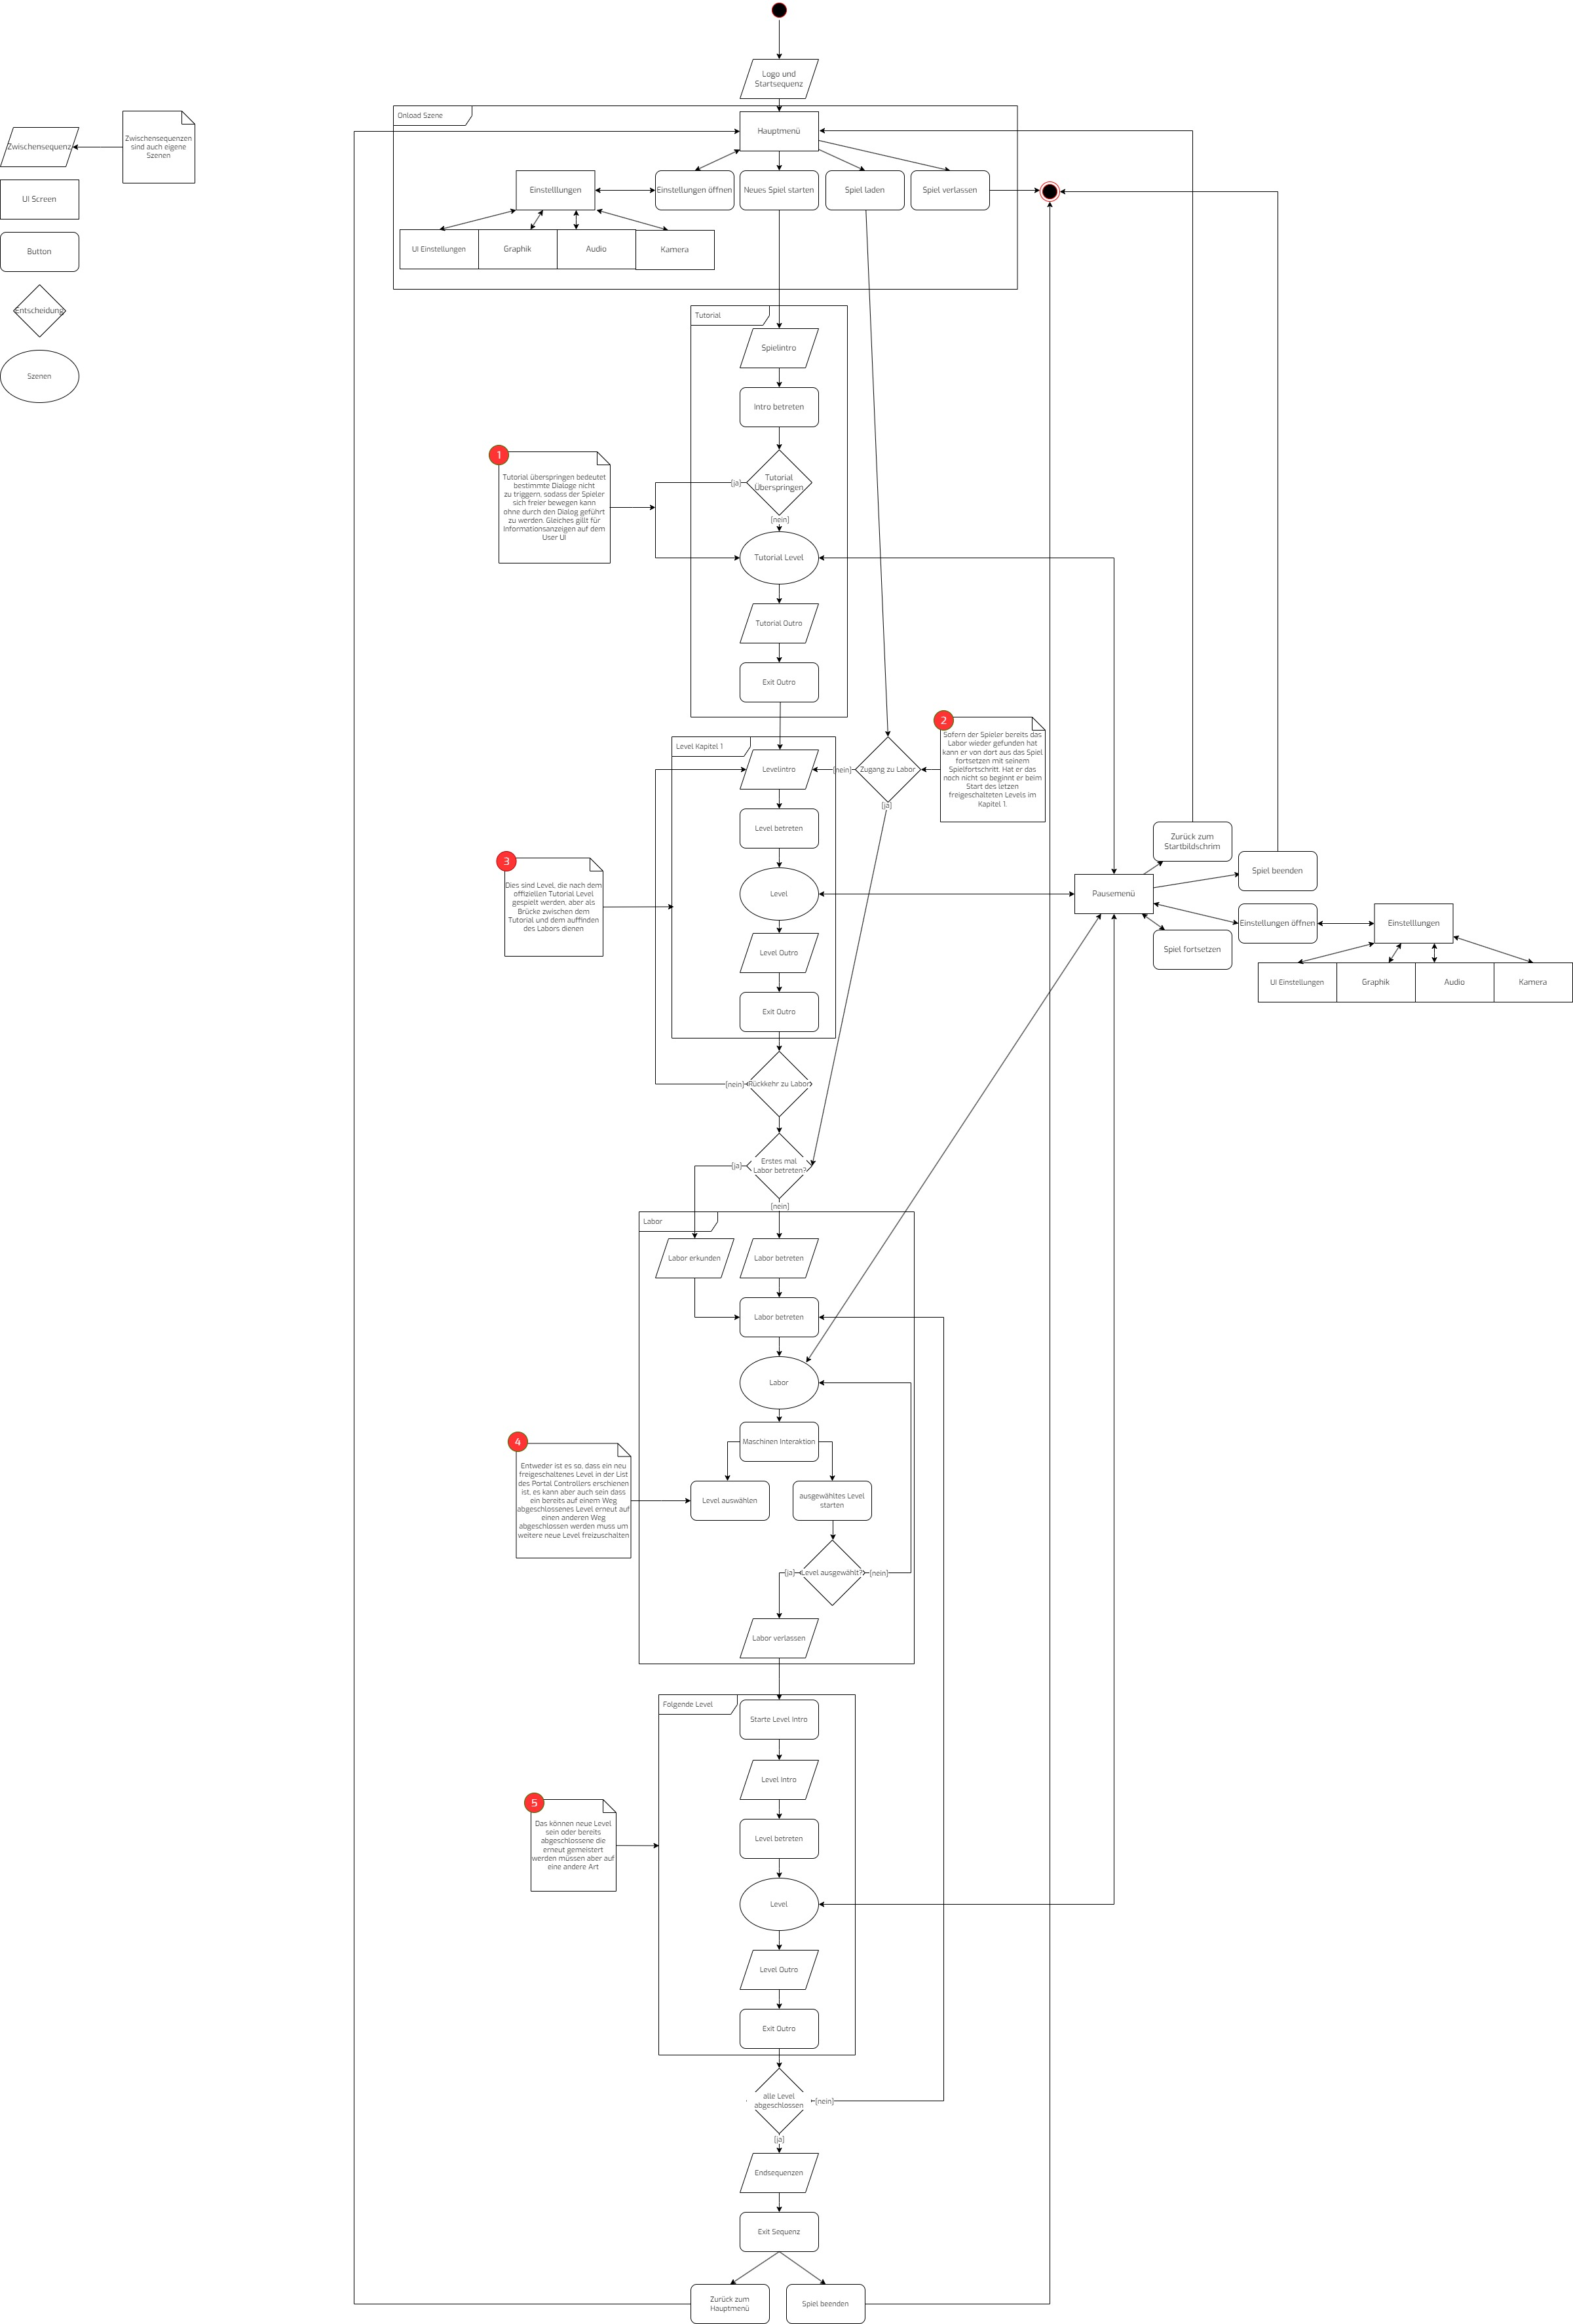
\includegraphics[width=0.5\linewidth]{content/pictures/main_loop.jpg}
\caption{Ablauf des gesamten Spiels (Quelle: eigene Darstellung)}
\label{fig:main_loop}
\end{figure}

Sobald das Spiel gestartet ist und das Startmenü geladen wurde, kann der Spieler zwischen vier verschiedenen Optionen auswählen. Zunächst kann er aus dem Hauptmenü heraus Einstellungen bezüglich der sichtbaren \ac{UI} tätigen, der Grafik, der Ton-Einstellung sowie der Kamera-Einstellung. Er kann das Spiel hier auch wieder beenden. Sofern der Spieler bereits einen Spielstand besitzt oder erzielt hat, kann er an diesem weiterspielen und würde entweder in seinem Labor beginnen, oder er startet das letzte freigeschaltete Level. Hat er das Spiel zum ersten Mal gestartet, so beginnt der Spieler im Tutorial. Zu Beginn des Tutorials kann der Spieler entscheiden, ob er das Tutorial Level als ein Tutorial spielen möchte, oder ob er das Level auf seine Art ohne den geführten Dialog meistern will. Mit geführtem Dialog bekommt der Spieler Hinweise über Objekte, die er anfangs betätigen muss. Zudem wird dem Spieler mitgeteilt, wie der Chronologe seine Erkenntnisse bezüglich der Mechanik des Spiels äußert. Dadurch wird dem Spieler erklärt, was bei den Prozessen des \say{\emph{Splittings}} und des \say{\emph{Mergings}} genau passiert und was diese Prozesse für eine Wirkung besitzen. Zudem erklärt der Chronologe so auch die Bedeutung der \ac{UI}, die der Spieler zur Laufzeit sehen kann. Der Spieler kann durch die Auswahl auch ohne diese Dialoge spielen. So erhält er nur über erhaltene Informationspakete Informationen über das Geschehen des Spiels. Diese Informationen werden auch bei einem geführten Tutorial an den Spieler übergeben.
Nach Abschließen des Tutorials erhält der Spieler ein Überblick über den Graphen, eine Bündelung aller entstandenen Zeitlinien zur Laufzeit des Levels, und welches Level er jetzt als Nächstes starten wird. Daraufhin sieht der Spieler in Form einer Zeichensequenz, wie der Chronologe durch ein Zeitportal geht und in eine weitere Zeitlinie übergeht. Bevor er nun das zweite Level starten kann, sieht der Spieler eine Zeichensequenz, wie der Chronologe die neue Spielwelt betritt und die Umgebung erkundet. Anschließend startet das Level für den Spieler. Die ersten fünf Level, inbegriffen das Tutorial, sind im selben Muster, wie es beim Tutorial beschrieben wurde aufgebaut. Im fünften Level erhält der Spieler Informationen, auf welche Weise er in sein Labor zurückreisen kann. Allerdings befindet sich dieses nicht da, wo es vor dem Start der Maschine war, sondern in einem Zwischenraum der unterschiedlichen Zeitlinien des Kontinuums. Aus dem Labor aus kann der Spieler nun die bereits abgeschlossenen Level erneut spielen und kann diese auf demselben Weg abschließen wie bislang, oder er kann durch das Besitzen weiterer verfügbaren Zeitlinien das Level auch durch einen anderen Weg freischalten, oder bislang unerreichbare Gegenstände einsammeln. Dadurch können neue Level freigeschaltet werden, um in der Spielhandlung voranzuschreiten. Über den Computer des Chronologen im Labor kann der Spieler seine Auswahl treffen und reist fortan in ausgewählte Zeitlinien. Auf diese Weise kann der Spieler nun von Spielwelt zu Spielwelt reisen, bis er das Ende der Story erreicht. Nach Beendigung des Levels kann er das gesamte Spiel neu starten oder an dem Spielstand nach dem letzten Level fortführen.

\subsection{Level Ablauf}

\begin{figure}[ht]
\centering
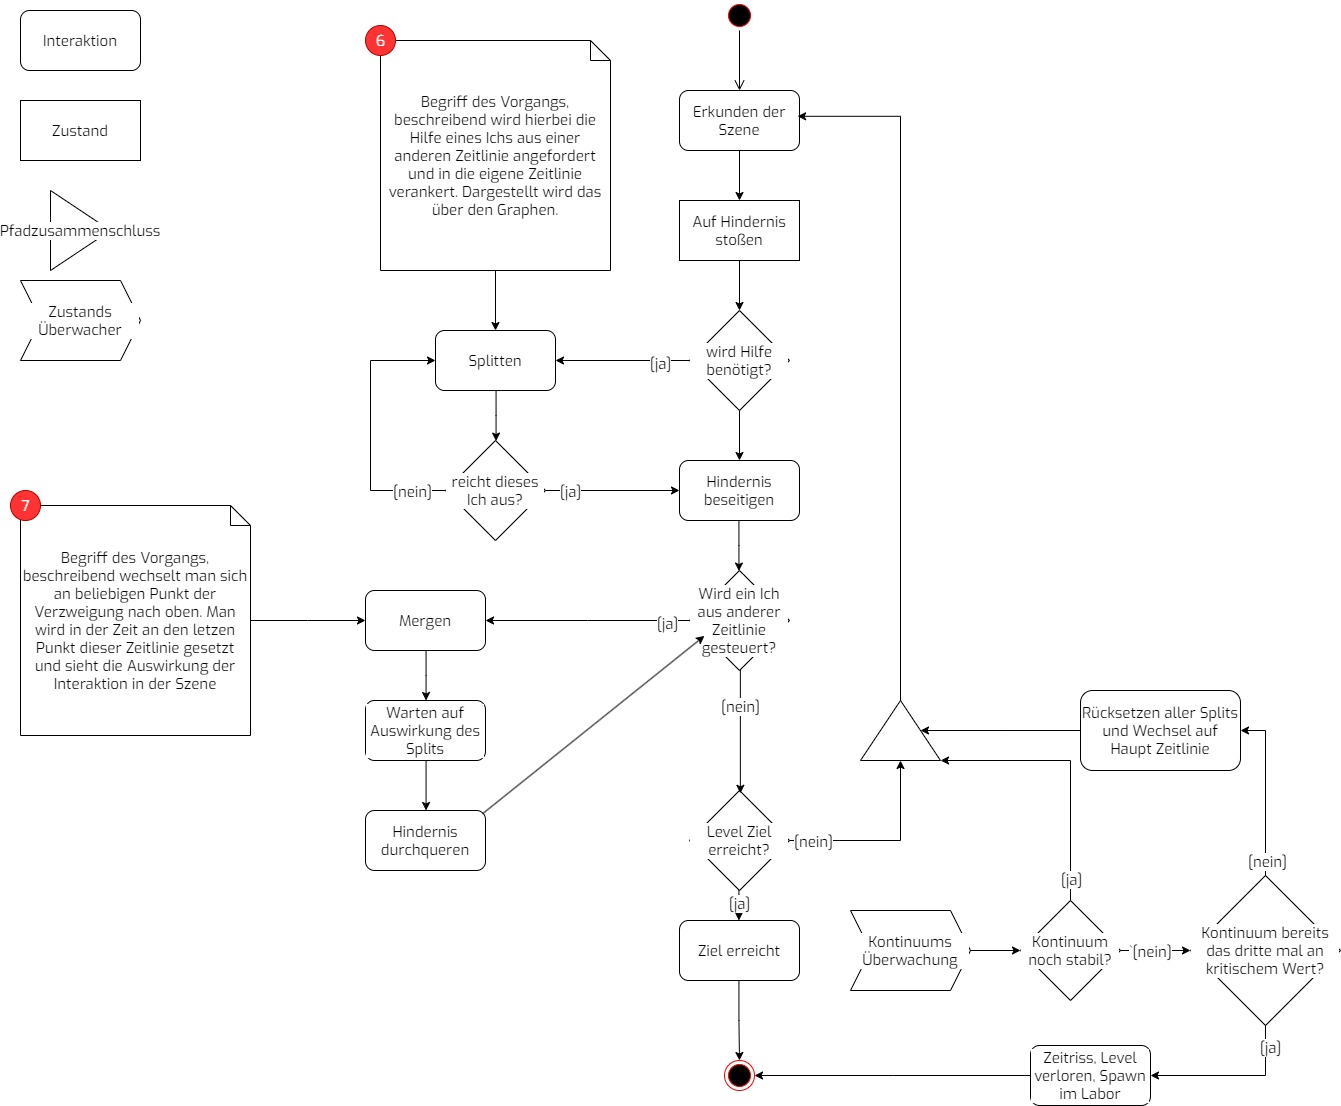
\includegraphics[width=0.3\linewidth]{content/pictures/level_loop.jpg}
\caption{Ablauf eines Levels (Quelle: eigene Darstellung)}
\label{fig:level_loop}
\end{figure}

Sobald das Level geladen wurde, wird der Spieler auf den Startpunkt des Levels gesetzt. Von dort aus steuert der Spieler den Chronologen in der Spielwelt, bis er auf ein Hindernis oder ein Rätsel trifft. Ab diesem Zeitpunkt muss der Spieler ein Ich aus einer anderen Zeitlinie über die Steuereinheit auswählen. Dadurch wird die Zeitlinie dieses Ichs an die Zeitlinie des Chronologen gehängt und der Spieler kann dieses Ich nun steuern. Auf diese Weise kann der Spieler den Mechanismus suchen und finden, welcher das Rätsel löst oder das Hindernis beseitigt. Bspw. muss er auf ein Gerüst klettern, auf welchem sich eine Druckplatte befindet, die eine verschlossene Tür öffnet. Sobald er sich auf die Druckplatte gestellt hat, wird genau zu diesem Zeitpunkt das Hindernis beseitigt. Dann kann er über die Steuereinheit den Chronologen der Hauptzeitlinie auswählen und sieht jetzt, wie die Tür durch die Druckplatte geöffnet wird. Solange das gesamte Level noch nicht absolviert ist und weitere Rätsel bzw. Hindernisse in den Weg gestellt werden, wird der Spieler diese, auf die eben beschrieben Weise lösen. Es ist möglich, dass der Spieler sein \say{Jump 'n´Run} Fähigkeiten beweisen muss, allerdings ist das nicht immer der Fall. Der Spieler wird primär damit beschäftigt sein, wie er seine Charaktere in die richtige Reihenfolge \say{\emph{Splitten}} muss, um die entsprechenden Rätsel zu lösen. Dabei hat er anfangs keine Zeitbegrenzung. Sein einziges Limit wird die Stabilität des Kontinuums sein, das er durch entsprechendes \say{\emph{Splitting}} und \say{\emph{Merging}} seiner diversen Chronologen beschädigen wird. Es wird allerdings auch Rätsel geben, an denen der Spieler seine Chronologen auf bestimmten Plattformen zu stellen hat, durch welche bestimmte Muster nachgebildet werden. 
Fällt die Stabilität des Kontinuums durch zu häufiges und zu langes Splitten dreimal an einen Grenzwert im roten Bereich, so entsteht eine Zeitlinienkonvergenz, durch welchen der Chronologe in der Zeit verloren geht und der Spieler das Level verliert. Nachdem der Spieler das Level neu gestartet hat, erscheint der Chronologe wieder in seinem Labor und der Spieler kann das Level erneut starten.
Die Begrifflichkeiten \say{\emph{Splitting}} und \say{\emph{Merging}} werden in ihrem entsprechenden Kapitel angesprochen.

\subsection{Labor Ablauf}
\begin{figure}[ht]
\centering
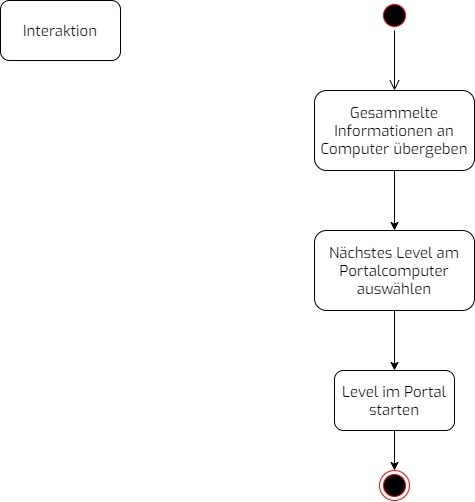
\includegraphics[width=0.3\linewidth]{content/pictures/labor_loop.jpg}
\caption{Ablauf des Labors (Quelle: eigene Darstellung)}
\label{fig:labor_loop}
\end{figure}

Nach dem Abschließen des ersten Kapitels, erhält der Spieler einen Hinweis, wie der Chronologe in sein Labor zurückreisen kann. Mit diesen Informationen kann der Spieler zum ersten Mal in sein Labor zurückreisen und von dort aus seine Reisen in andere Zeitlinien starten. Das Labor dient dem Spieler künftig als Hub. Beim erstmaligen Betreten des Labors wird der Chronologe das Labor nach Schäden jeglicher Art absuchen. Er stellt dabei fest, dass alles noch so aussieht, wie beim Start der Maschine. Als Erstes überträgt er seine gesammelten Notizen der ersten Level in seinen Computer. Über den Computer wird der Spieler noch mehr Informationen über die Welten erhalten. Der Computer kann aus den erhaltenen Informationen Rückschlüsse über die Welt herführen, die der Spieler auslesen und verwenden kann. Nachdem der Chronologe seine gesammelten Notizen an seinen Computer übertragen hat, kann der Spieler an der Steuereinheit der Maschine im Labor positioniert und das nächste Level auswählt. Im Anschluss kann er das Portal betreten und starten. Auf diese Weise wird der Spieler in weitere Level der verschiedenen Zeitlinien wechseln können. Einige Level sind dabei jeweils in derselben Zeitlinie, sie können manchmal auch vor oder nach dem zuvor gespielten Level in der Zeithierarchie stattfinden. Nach jedem erfolgreich abgeschlossenen Level geht der Chronologe zuerst an seinen Computer und trägt seine Funde in sein System ein. Sobald der Spieler ein Level aufgrund eines zerstörten Zeitkontinuums verliert, wird er wieder im Labor landen, allerdings so als ob sein Versuch niemals stattgefunden hätte.

\section{Zeitkontinuum}
Das Zeitkontinuum ist die überwachende Instanz des gesamten Spiels. Sie misst Auswirkungen und Einflüsse aller parallelen Zeitlinien dieser Spielwelt. Solange die Zeitlinien in sich geschlossen bleiben und nicht versucht wird, miteinander Kontakt aufzunehmen, kann das Kontinuum nicht gefährdet werden. Anders ist es jedoch, wenn versucht wird, die Barriere der Zeitlinien zu durchbrechen und zu erforschen, wie andere Szenarien aussehen würden, wenn andere Entscheidungen getroffen worden wären. Ein dadurch entstehendes Wanken und Beschädigen des Kontinuums hat zur Folge, dass Zeitlinien nicht nur für Einflüsse von anderen Zeitlinien anfällig werden, sondern zusätzlich auch noch für Einflüsse aus der Zukunft oder der Vergangenheit. Durch die Wirkung anderer Zeitlinien steigt die Gefahr der Entstehung von Paradoxen. Das Zeitkontinuum kann eine begrenzte Anzahl von Paradoxen durch ihre Stärke kompensieren. Zu viele Paradoxen sollten sich in den verschiedenen Zeitlinien allerdings nicht bilden, sonst kann es passieren, dass das Kontinuum zerfällt und es zu Konvergenzen der Zeit kommt. Da das Kontinuum ein allumfassendes Konstrukt ist, wird es für den Gebrauch dieses Spiels die Zeitlinie des Chronologen betrachten, der dem Bestreben nachging, parallele Zeitlinien zu erforschen. Diese Zeitlinie gilt von nun als Hauptbezugspunkt des Kontinuums. Allerdings bezieht es seine Auswirkungen auf das Gebiet aller anderen Zeitlinien ebenfalls mit ein, wie die Auswirkungen auf die Zeitlinie des Chronologen. Das Kontinuum überwacht dabei das Entstehen von Paradoxen, die der Chronologe durch das Nutzen seiner Steuereinheit versehentlich erzeugen kann. Zudem misst es, ab welchem Zeitpunkt das Parallelisieren von Zeitlinien auf einer Zeitlinie zu Konvergenzen in der Zeit führen kann.

\subsection{Zeitlinienkonvergenz}\label{sec:konvergenz}
Die Zeitlinienkonvergenz ist eine Katastrophe, die entsteht, wenn die Stabilität des Kontinuums zu häufig auf einen gekennzeichneten Tiefpunkt gerät. Dadurch kann das Kontinuum die verschiedenen Zeitlinien und die Zeit nicht mehr ordnen und fallen alle auf eine Zeitlinie und auf einen Zeitpunkt. Dadurch wird das ganze Kontinuum zerstört. Sobald eine Zeitlinienkonvergenz entsteht, verliert der Spieler das aktuelle Level und wird entweder zurück in das Labor versetzt oder er muss das zuvor gestartete Level neu starten.

\subsection{Graph}
Der Graph ist ein Gerüst in dieser Konzeption und dient als Unterstützung bzw. Visualisierung des Zeitkontinuums, das auf die Zeitlinie des Chronologen gerichtet ist. Er dient visuell der Darstellung der \say{\emph{erzeugten}} Zeitlinien, die in abhängiger Verästlung an die Bezugszeitlinie des Kontinuums gehängt wird. Dabei sind diese Zeitlinien im Geflecht eines gesamten Kontinuums nicht \say{\emph{neu}} sondern lediglich in diese Zeitlinie integriert, sodass der Chronologe aus dieser Zeitlinie in der aktuellen Zeitlinie interagieren kann. Auf technischer Seite dient der Graph der Strukturierung der Zeitlinien. Durch ihn kann man feststellen, wann und in Bezug auf welche andere Zeitlinie man eine integrierte Zeitlinie nutzen möchte. Den entstehenden Graphen kann der Spieler jederzeit betrachten und inspizieren. Durch eine Zeitskala kann der Spieler sehen, zu welchem Zeitpunkt des Spiels er welche Zeitlinie ausgewählt hat und wie lange diese Zeitlinie integriert wurde. Einen endgültigen Überblick über den Graphen erhält der Spieler nach erfolgreichem Absolvieren eines Levels des Spiels. Dieser Graph kann sich von dem dargestellten Graphen, den der Spieler zur Laufzeit einsehen kann, unterscheiden, da er bereits laufende Zeitlinien unterbrechen oder abbrechen kann. Dazu in Abschnitt \say{\emph{Zeitlinien löschen}} mehr.

\subsection{Zeitlinie}
Eine Zeitlinie beschreibt den Verlauf eines Lebens einer Person und die Leben der Personen, die in genau dieser Umgebung leben. Jede Entscheidung, die dabei getroffen wird, hat einen Einfluss auf jedes Leben aller Personen in dieser Zeitlinie. Im Kontext der Konzeption dieses Spiels bildet die Zeitlinie das Leben eines Ichs des Chronologen ab, welches der Spieler später steuern wird. Man kann festhalten, der Chronologe hat vor, in das Leben eines anderen Ichs einzutauchen, um zu erfahren, wie das Leben aus der Perspektive dieses Ichs wäre, wenn andere Entscheidungen getroffen worden wären. Dabei sähe der Chronologe ebenfalls eine andere Welt, die andere Ereignisse in der Vergangenheit erlebt hat und auch andere Ereignisse in der Zukunft erleben wird. Im Kontext dieses Spiels werden diese Zeitlinien in der Zeitlinie des Chronologen verankert. Dadurch entsteht der Effekt, dass Zeitlinien und ihre Ichs der Chronologen interaktiv mit der Zeitlinie des Haupt-Chronologen zusammenarbeiten können. Infolgedessen kann durch diesen Ansatz und dieses Verständnis auf der technischen Entwicklungs-Seite eine Abhängigkeit zwischen Zeitlinien erzeugen, auf welchen die gesteuerten Ichs des Chronologen abgebildet werden. Jede Zeitlinie bleibt in sich geschlossen und eigenständig, allerdings kann durch ein Konstrukt wie den Graphen eine Abhängigkeit voneinander erzeugt werden, welche für eine spätere Umsetzung notwendig ist.

\subsubsection{Splitting}\label{sec:split}
\say{\emph{Splitting}} bedeutet in dem Kontext dieses Spiel das Erzeugen einer neuen Zeitlinie, auf der ein Ich des Chronologen lebt und gesteuert werden kann. Diese Zeitlinie wird an die bestehende Zeitlinie als Sublinie angehängt, wodurch eine Abhängigkeit zwischen den Zeitlinien entsteht.

\begin{figure}[ht]
\centering

\includegraphics[width=0.5\linewidth]{content/pictures/Split.jpg}
\caption{Neu entstandene Zeitlinie nach Split (Quelle: eigene Darstellung)}
\label{fig:split}
\end{figure}

Diese neu erzeugte Zeitlinie wird nun an die bisherige Zeitlinie angehängt. Dabei ist diese Zeitlinie keinesfalls neu, sondern lediglich die bislang bereits bestehende Zeitlinie eines Ichs des Chronologen, die in die Zeitlinie des Chronologen gelegt wird. Diese Zeitlinie besteht so lange, wie der Spieler das Ich des Chronologen steuert.
\begin{figure}[ht]
\centering

\includegraphics[width=0.5\linewidth]{content/pictures/Timeline.jpg}
\caption{derzeitige Zeitlinie (Quelle: eigene Darstellung)}
\label{fig:timeline}
\end{figure}
Durch mehrmaliges Splitten ergibt sich solch ein Schaubild:
\begin{figure}[ht]
\centering

\includegraphics[width=1\linewidth]{content/pictures/Merge.jpg}
\caption{Entstehender Baum (Graph) mit Verzweigungen (Zeitlinien) (Quelle: eigene Darstellung)}
\label{fig:graph}
\end{figure}
Wie in Abbildung \ref{fig:graph}: \nameref{fig:graph} zu sehen ist, ergibt sich daraus eine aneinander Reihung der eingegliederten Zeitlinien. Durch das Konstrukt des Graphen ist es nun möglich, diese angegliederten Zeitlinien auf technischer und visueller Ebene darzustellen und zu nutzen.
Nach einem \say{\emph{Split-Vorgang}} werden die Bewegungen und Interaktionen des Ichs des Chronologen aufgenommen, sodass diese nach einem \say{\emph{Merge-Vorgang}} abgespielt werden können und einen Einfluss auf die Spielwelt haben. Jede Bewegung und Interaktion bekommen dabei einen eindeutigen Zeitpunkt, um sie später reproduzieren zu können.

\subsubsection{Merging}\label{sec:merge}
\say{\emph{Merging}} beschreibt den Vorgang des Zurückspringens von einer neu erstellten Zeitlinie auf eine bereits existierende. Daraus folgend werden die aufgenommenen Bewegungen und Interaktionen anhand ihres Zeitpunktes genau reproduziert.
\begin{figure}[ht]
\centering
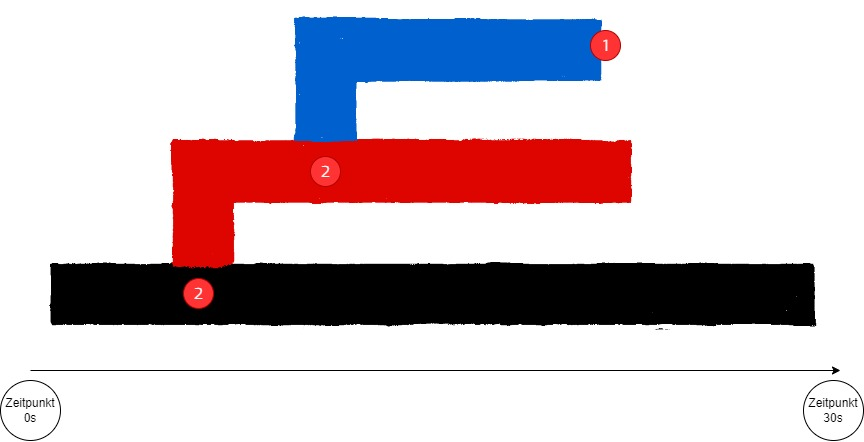
\includegraphics[width=1\linewidth]{content/pictures/merge_definition_grafik.jpg}
\caption{Entstandener Baum mit Knotenpunkten (Quelle: eigene Darstellung)}
\label{fig:merge-definition}
\end{figure}
Nach jedem \say{\emph{Split-Vorgang}} wird eine \say{neue} Zeitlinie an die bislang bestehende angesetzt. Daraufhin entsteht an dem Zeitpunkt, an dem die Zeitlinie ihre Verbindung erhält, ein Knotenpunkt (vgl. Abbildung \ref{fig:merge-definition}: \nameref{fig:merge-definition}, Markierung 2). Wenn der Spieler sich nach einem \say{\emph{Split}} an der Markierung 1 in Abbildung \ref{fig:merge-definition}: \nameref{fig:merge-definition} befindet, so kann er für einen, \say{\emph{Merge-Vorgang}} das Ich aus der roten oder der schwarzen Zeitlinie auswählen. Aus der Sicht der Spielzeit wird der Spieler jetzt an den Punkt zurückgesetzt, an denen einer der Knotenpunkte (Markierung mit der Zahl zwei) liegt. Wählt er beispielhaft den Knotenpunkt auf der schwarzen Zeitlinie aus, so wird zum selben Zeitpunkt die rote Zeitlinie aktiv und das Ich der roten Zeitlinie erscheint in der Szene. Nach einer bestimmten Zeit wird die blaue Zeitlinie aktiv und das Ich dieser Zeitlinie wird ebenfalls erscheinen. Diese Knotenpunkte entstehen nur bei einer Verankerung einer weiteren Zeitlinie an die derzeitige. 

\subsubsection{Paradoxen} 
Paradoxen können auftreten, indem der Spieler einer aufgezeichneten und bereits in der Welt verankerten Zeitlinie die Zustände der Spielwelt verändert. Das kann zum Beispiel dann passieren, wenn dem \say{Ich} dieser verankerten Zeitlinie Gegenstände in den Weg gestellt werden, gegen die dieser Charakter nun stoßen wird. Aufgrund der Tatsache, dass dieser Zustand bei der Aufnahme der Zeitlinie nicht gegeben war, entsteht nun ein Paradoxon, das dazu führt, dass die aufgenommene Zeitlinie und die an ihr angehängten Zeitlinien nun aus dem Kontinuum entfernt werden und dem Kontinuum Schaden zuführen. Diese Schäden spiegeln sich in der Veränderung der Welt wider, die in \say{Kapitel \ref{sec:paradoxon-stability}: \nameref{sec:paradoxon-stability}} näher beschrieben wird. Durch zu viele entstehende Paradoxen kann es auch dazu kommen, dass es zu einer Zeitlinienkonvergenz kommt, durch welche der Spieler das Level erneut starten muss. Ein weiteres Beispiel wäre z.B., wenn der Spieler während der \say{\emph{Splitphase}} einen Hebel betätigen würde, der bislang noch inaktiv war. Nachdem er durch das \say{\emph{Merging}} an einen Knotenpunkt zurückgesprungen ist, hätte er nun die Möglichkeit diesen Hebel ebenfalls zu betätigen. Tut der Spieler dies, bevor das Ich des aufgenommenen Charakters an den Hebel gelangt und hält ihn aktiv, bis dieser ihn aktivieren würde, so würde ein Paradoxon entstehen. Der Zustand des Hebels wurde nun geändert und führt dazu, dass ein inaktiver Hebel nicht mehr aktiviert werden kann. Das folgende Paradoxon würde die Gefahr einer auftretenden Zeitlinienkonvergenz vergrößern.

\subsubsection{Zeitlinien löschen}
Bereits eingegliederte Zeitlinien können nicht erneut eingegliedert werden, solange sie schon eingegliedert sind. Das bedeutet, würde der Spieler sehen, dass er zu kurz auf einer Druckplatte stehen geblieben ist, so müsste er die Zeitlinie löschen und damit in Kauf nehmen, dass das Kontinuum einen Schaden davontragen werde, um das Ich der Zeitlinie erneut und für eine längere Zeit auf die Druckplatte zu stellen. Gleichwohl kann er das auch machen, wenn er mit der Aufnahme der Zeitlinie nicht zufrieden ist und mehrmals an einer Stelle gestürzt ist und einen Parcours nicht erfolgreich meistern konnte.

\subsection{Timer}
Der Timer zeigt dem Spieler an, wie lange er bereits in dem Level spielt. Er dient als Orientierung, ab welchem Zeitpunkt bis zu welchem Zeitpunkt der Spieler mit einem Ich aus einer anderen Zeitlinie spielt. So kann er abschätzen, wann die Zeitlinie seines gespeicherten Ichs nicht mehr in der Welt verfügbar ist und wann dementsprechend der Charakter der Zeitlinie nicht mehr bspw. auf einer Druckplatte stehen wird. Der Timer ist die zählende Komponente des Spiels, über die das Zeitkontinuum wacht. Durch den Timer kann nun auch bestimmt werden, wann eine Zeitlinie aus dem Kontinuum an die Zeitlinie des Chronologen angegliedert wird und wann der Spieler durch das \say{\emph{Merging}} an einen Knotenpunkt zurückgesprungen ist, also gewissermaßen wieder in die Vergangenheit gereist ist.

\subsection{Charaktere}
Der Spieler sieht im  Spiel über die Steuereinheit die Namen seiner Ichs aus anderen Zeitlinien. Über eine Ansicht der verschieden verfügbaren Zeitlinien erhält er ebenfalls nur die Ansicht des Ichs aus dieser Zeitlinie. Ein Charakter ist in dem Kontext des Spiels der eigentliche Chronologe aus der fokussierten Zeitlinie des Kontinuums und seine abgewandelten Persönlichkeiten aus den erforschten Zeitlinien. Der Spieler steuert jeweils das Selbst des Chronologen in all seinen Facetten.

\subsection{Bewegungen und Interaktionen}
Der Spieler wird durch den Chronologen die Spielwelt erkunden. Dabei kann der Chronologe mit Gegenständen wie z.B. Hebeln interagieren. Er kann Gegenstände tragen, er kann an bestimmten Stellen auf Gegenstände klettern und er kann sie verschieben. Zudem ist es ihm möglich auf Objekte zu stehen und diese dadurch zu aktivieren. Außerdem kann er, über kleinere Abgründe hinwegspringen und rennen. All diese Bewegungs- und Interaktionsmöglichkeiten werden auf der Zeitlinie des ausgewählten Chronologen gespeichert und mit einem Zeitpunkt versehen, damit diese chronologisch wieder rekonstruiert werden können. Steuert der Spieler den Haupt-Chronologen, so werden seine Bewegungen und Interaktionen nicht aufgenommen.

\subsection{Einflüsse auf die Spielwelt}\label{sec:paradoxon-stability}
Ein instabiles Zeitkontinuum hat direkte Auswirkungen auf die Spielwelt, in der sich der Spieler mit dem Chronologen befindet. Durch die Gegebenheit, dass es viele verschiedene Zeitlinien gibt, die parallel verlaufen, existieren auch viele verschiedene Version des Raumes bzw. des Ortes, an dem sich der Spieler jetzt gerade in dem Moment befindet. Durch ein instabiles Zeitkontinuum sind die Grenzen der in sich geschlossenen Zeitlinien brüchig und können auf andere Zeitlinien übergehen. Das hat zur Folge, dass Gegenstände oder gar Wandelemente plötzlich in der Spielwelt auftauchen und manche Bereiche des Levels nicht mehr betreten werden können, da an dieser Stelle plötzlich eine Wand erscheint. Es kann allerdings auch dazu führen, dass Elemente aus der Spielwelt verschwinden und plötzlich in einer anderen Zeitlinie in einer anderen Umgebung auftauchen. Der Spieler muss also Sorge tragen, dass durch sein Handeln die Spielwelt nicht beschädigt wird. Durch eine Beschädigung würde der Spieler ein Level verlieren oder ihm würden unüberwindbare Hindernisse in den Weg gestellt werden. Er muss warten, bis sich das Kontinuum wieder erholt hat. Der Spieler wird das Erholen des Zeitkontinuums anhand einer Anzeige auf seinem \ac{UI} sehen. Dies wird im Kapitel \say{\ref{sec:kontinuum_ui}: \nameref{sec:kontinuum_ui}} visualisiert.

Unabhängig von der Instabilität des Kontinuums kann sich die Welt aus der Perspektive der anderen Ichs des Chronologen auch verändern. Jedes Ich ist in seiner Zeitlinie unterschiedlich zu anderen Zeitlinien. Das bedeutet auch, dass diese Ichs bestimmte Dinge auf eine andere Art wahrnehmen oder andere Dinge sehen können. Zum Beispiel können sich bestimmte Dekorationsobjekte unterscheiden oder Teile der Wände sind anders. So wird sich das Leveldesign aus Sicht der Ichs des Chronologen teilweise unterscheiden. Die Kernelemente der Rätsel bleiben jedoch aus jeder Sicht der Ichs identisch. So wird einer Verwirrung des Spielers vorgebeugt.

\section{Belohnungen}
Nach Abschließen eines Levels, erhält der Spieler das Ich des Chronologen aus dieser Zeitlinie zur Auswahl als Belohnung. Damit hat er für die kommenden und bereits absolvierten Rätsel eine Auswahlmöglichkeit mehr, seine Ichs anzuordnen. Das ermöglicht dem Spieler, die Level über ein anderes Ziel abzuschließen.

\section{Labor}
Nachdem der Spieler nach Abschließen des ersten Kapitels der Story das Labor wieder entdeckt hat, kann er von dort aus bereits abgeschlossene Level erneut starten und zu neuen Levels reisen. Außerdem kann der Chronologe seine Erkenntnisse aus den abgeschlossenen Level hier abspeichern und erfährt dadurch mehr über die Spielwelten, in welche er reist.

\section{Aufnahmen des Chronologen}\label{sec:npc}
Im Kontext dieses Spiels unterscheiden wir zwischen zwei Arten von \say{None-Playable} Charakteren, die ein Abbild des Chronologen darstellen, aber nicht vom Spieler gesteuert werden. Es wird im Sprachgebrauch von Platzhaltern und Geistern gesprochen.

\subsection{Platzhalter}
Sobald der Spieler in ein anderes Ich des Chronologen springt, wird an der letzten Stelle, an dem sich der bisherige Spielercharakter befand, ein Platzhalter gesetzt. Dieser Platzhalter dient dazu, zu zeigen, dass sich dieses Ich des Chronologen in der Zeit noch nicht fortbewegt hat, genauer gesagt zu diesen Zeitpunkten, die der Spieler nach dem \say{\emph{Splitting}} erlebt, noch nicht erlebt hat. Der Chronologe, der vor dem \say{\emph{Mergeprozess}} noch ein Platzhalter war, wird nach dem \say{\emph{Mergeprozess}} diese kommenden Zeitpunkte erleben. Er besitzt eine durchscheinend transparente Gestalt, welche dem Spieler vermittelt, er würde zum einen an dieser Stelle wieder beginnen und zum anderen auch anzeigen, dass dies kein paralleler Chronologe ist.

\subsection{Geister}
Nach einem \say{\emph{Merge-Prozess}} wird der Chronologe der gespielten Zeitlinie in die Spielwelt verankert.
Er besitzt das Aussehen des Ichs des Chronologen, das der Spieler bereits beim Spielen des Ichs gesehen hat. Dies zeigt an, dass das Ich des Chronologen, den der Spieler gesteuert hat, die aufgenommenen Interaktionen und Bewegungen ausführt. Er ist die kooperative Komponente des Spiels. Auf das Verhalten dieses Ichs kann der Spieler nun reagieren, um die laufenden Rätsel zu lösen. 
Alle 3D Modelle des Chronologen, die nicht transparent sind, haben einen direkten Einfluss auf die Spielwelt und das Kontinuum.

\section{Gebrauchsgegenstände}
Zu Beginn des Spiels besitzt der Chronologe zwei Gebrauchsgegenstände, die auf die anderen Ichs des Chronologen übertragen werden können. Durch diese kann der Spieler seine im Labor befindliche Maschine ferngesteuert bedienen und er kann seine notierten Erkenntnisse und Notizen über die Welt notieren.

\subsection{Steuereinheit}
Seine Erfindung im Labor besitzt eine Steuereinheit, um sie zu bedienen. Sie ist Teil seines Computers, der ebenfalls im Labor steht. Um seine Maschine auch außerhalb des Levels zu bedienen, hat er eine mobile Steuereinheit entwickelt. Durch diese kann der Spieler die verschiedenen Versionen des Chronologen überblicken und auswählen. Er erhält dadurch eine Übersicht über die Namen und den derzeitigen Status in der Szene der Ichs.

\subsection{Datenleser}\label{sec:concept_datenleser}
Über den Datenleser kann der Chronologe seine Erkenntnisse und Notizen sammeln. Der Spieler kann diesen Datenleser öffnen, um über ihn Informationen über die Welt und die einzelnen Zeitlinien zu bekommen. Zusätzlich werden wichtige Abläufe und Informationen des Spiels darüber einsehbar. Der Spieler kann ihn, als Journal nutzen, um Wissen über das Spiel zu sammeln.

Im Laufe der Handlung des Spiels und beim wachsenden Fortschritt der Erkundung der verschiedenen Zeitlinien erhält der Chronologe weitere Gegenstände, die ihm, als Hilfsmittel zur Lösung der Rätsel dienen. Durch den Erhalt von neuen Gebrauchsgegenständen steigt die Anforderung des Spiels an den Spieler. Er muss diese Gegenstände nun zielführend einsetzen, um die Rätsel lösen zu können. Er kann dadurch seinen Spielfluss verbessern, allerdings wird seine Umgebung auch herausfordernder.

\subsection{Imitator}\label{sec:concept_imitator}
Der Chronologe findet im Laufe des Spiels die Auswirkungen der Steuereinheit auf den Ablauf immer besser kennen. Daher beschließt er, mit der Hilfe und den Informationen aus den Ichs der anderen Zeitlinien einen Imitator zu bauen, der begrenzt nutzbar einen Platzhalter auf eine Druckplatte oder Ähnliches stellt. Dadurch muss der Spieler keinen \say{\emph{Split}} ausführen und auf der Druckplatte warten, bis sein Ich nach einem \say{\emph{Merge}} über den daraus resultierenden Freiraum gegangen ist. Wie bereits erwähnt, führen viele \say{\emph{Splits}} und \say{\emph{Merges}} zu einer Instabilität des Kontinuums. Dieser Imitator soll das verhindern, er kann aber nicht so oft genutzt werden. Er soll lediglich an den bestimmten Stellen nützlich sein, an denen es zu einer Knappheit der verfügbaren Ichs in der Steuereinheit kommt oder die Gefahr besteht, das Level zu verlieren. 

Durch den Imitator kann der Spieler seine Auswirkungen auf das Kontinuum schonen. Zusätzlich kann er durch den ihn genau wissen, wie lang eine Kopie seiner selbst an diesem Punkt steht.

\subsection{Pager}
Einen Pager findet der Spieler auch zu einem bestimmten Zeitpunkt des Spiels gegen Ende der Story. Zu diesem Zeitpunkt sind die Rätsel komplexer geworden und der Spieler muss seine \say{\emph{Splits}} und \say{\emph{Merges}} nun genau abstimmen, damit zum richtigen Zeitpunkt die richtigen Auswirkungen auf die Spielwelt ausgeführt werden können. Ein Pager hilft ihm, seinem zu steuernden Chronologen nach einem \say{\emph{Merge}} Bescheid zu geben, wann bspw. ein Hebel umgelegt wird. Der Spieler erhält dabei eine Nachricht, die wie folgt aussehen kann: \say{[Chronologe Ich Variante] legt jetzt Hebel um}. Durch diese erhaltene Nachricht weiß er nun, wann der Hebel umgelegt wird, und kann darauf reagieren. Sofern der derzeitig gesteuerte Chronologe nicht der ursprüngliche Chronologe ist, kann der Spieler nun auch weiteren zu steuernden Chronologen eine Nachricht senden. Jede Ich-Variante des Chronologen kann also sowohl Nachrichten empfangen als auch Nachrichten versenden. Der ursprüngliche Chronologe kann jedoch nur Nachrichten empfangen, um darauf zu reagieren.

\section{Leveldesign}
Ein großer Teil des Spiels beruht auf dem Leveldesign der einzelnen Schauplätze, in denen die verschiedenen Rätsel integriert sind. Im Folgenden werden die bisher umgesetzten Rätsel und ihre Lösungen aufgezählt und vorgestellt. Zudem wird es einen Ausblick darauf geben, welche weiteren Rätsel bereits konzipiert und noch nicht gelöst wurden. Des Weiteren wird beschrieben, welche weiteren Rätsel für das Spiel möglich wären.

In einem weiteren Teil werden die Objekte, mit denen interagiert werden kann, beschrieben. Diese werden im Folgenden aufgelistet. Im Abschnitt \ref{sec:design} dieser Thesis werden diese Objekte visuell dargestellt.

\subsection{Interaktionsobjekte}
In den Spielwelten des Spiels gibt es verschiedene Objekte, mit denen der Chronologe interagieren kann. Im Folgenden werden diese Objekte konzeptionell vorgestellt.

\subsubsection{Druckplatte}
Druckplatten befinden sich auf dem Boden und können durch das Körpergewicht des Chronologen ausgelöst werden. Nachdem Druckplatten ausgelöst wurden, aktivieren diese weiteren Objekte wie  Türen, Kräne oder Plattformen an der Wand. Verlässt der Spieler die Druckplatte, so deaktiviert sie sich und ihre verknüpften Objekte. Eine Druckplatte bleibt nur aktiv, sobald ein Ich des Chronologen auf ihr steht. 

\subsubsection{Hebel}
Hebel können sich auf dem Boden oder an Wänden befinden. Der Spieler kann ebenfalls mit diesem interagieren. Der Chronologe drückt den Hebel-Stab auf seine aktive Position. Diese muss der Chronologe halten. Solange der Hebel-Stab auf der aktiv Position des Hebels steht, ist der Hebel wirksam. Dadurch können Lampen angestellt werden, Tore geöffnet oder Plattformen aktiviert werden. Entfernt sich der Spieler aber zu weit vom Hebel weg, deaktiviert sich dieser und seine verknüpften Objekte werden ebenfalls deaktiviert. Zum Beispiel schließt sich eine Tür oder ausgefahrene Plattformen fahren wieder ein.

\subsubsection{Ventil}\label{sec:ventil}
Ventile befinden sich an der Wand oder an Rohren. Sie dienen dazu, um entweder Rohrflüsse zu aktivieren oder um bewegliche Plattformen zu verschieben. Durch einmalige Interaktion mit einem Ventil ist sowohl der Rohrfluss geöffnet oder geschlossen als auch die Plattform an ihrem entsprechenden Zielort.

\subsubsection{Kletterkanten}
Der Chronologe kann auf höher gelegene Objekte klettern. Diese Objekte, wie  Plattformen oder Stützen, besitzen eine greifbare Kante, an der sich der Chronologe hochziehen kann. 

\subsubsection{Tragbare Objekte}
Dem Chronologen ist es möglich, bestimmte Objekte zu tragen. Dadurch kann er Klettermöglichkeiten für einen anderen Spieler erzeugen, oder für sich selbst Vorrichtungen bauen, um über Abgründe hinwegzuspringen.

\subsubsection{Portal Steuereinheit}
Im Labor befindet sich eine stationäre Steuereinheit seiner Maschine. Diese dient dazu, das nächste Ziel oder das nächste Level in einer Zeitlinie auszuwählen. Aktiviert er nun die Maschine in einem geschaffenen Portal, so wird er an das Ziel befördert.

\subsubsection{Objekte zum Schieben}
Der Chronologe kann nicht nur bestimmte Objekte tragen, sondern auch schieben. Dadurch kann er etwa Wege freiräumen oder vorteilhaftere Positionen schaffen, von denen der Chronologe auf höher gelegene Objekte klettern kann.

\subsection{Rätsel}
Die Rätsel der einzelnen Spielwelten können variieren. Es gibt Abschnitte, in denen durch Betätigen einzelner Abschnitte andere Abschnitte freigelegt werden. Es kann aber auch sein, dass durch das Anwenden eines \say{\emph{Split}}- und \say{\emph{Merge}}-Vorganges der richtige Weg ans Ziel gefunden werden muss. Oder aber es ist notwendig, zu bestimmten Zeitpunkten, mit den richtigen Ichs des Chronologen an bestimmten Stellen zu stehen, um Mechanismen auszulösen. Anschließend wird das Rätseldesign vorgestellt. Dabei wird zwischen bereits umgesetzten und konzipierten Rätseln unterschieden.

% Dieser Abschnitt enthält Spoiler und Lösungen.
\subsubsection{Umgesetzte Rätsel}
Im Folgenden werden nun die umgesetzten Rätsel mit ihrer jeweiligen Lösungsmethode vorgestellt. 

Im Tutorial hat der Spieler zwei weitere Ichs des Chronologen zur Auswahl. Diese drei verschiedenen Zeitlinien haben eine jeweils eindeutige Farbe.

\paragraph{Tutorial, Raum 1:}
% \medskip

\begin{figure}[ht]
\centering
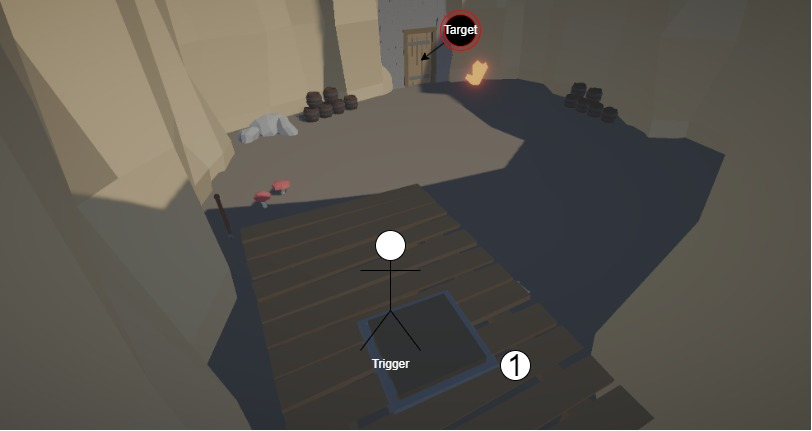
\includegraphics[width=0.8\linewidth]{content/pictures/Raetsel-L01_R01_R01.jpg}
\caption{Rätsel im ersten Tutorial Raum (Quelle: eigene Darstellung)}
\label{fig:L01_R01_R01}
\end{figure}

Zu Beginn trifft der Spieler auf eine verschlossene Tür (siehe Abbildung \ref{fig:L01_R01_R01}: \nameref{fig:L01_R01_R01}). Über die Druckplatte auf dem Gerüst kann der Spieler die Tür öffnen. Dazu muss er auf das Gerüst klettern, das ohne Probleme funktioniert. Um final mit dem Chronologen durch die Tür zu gelangen, muss der Spieler ein weiteres Ich des Chronologen zur Hilfe nehmen, der daraus resultierende Graph in Abbildung \ref{fig:L01_R01_R01_L}: \nameref{fig:L01_R01_R01_L} hat eine solche Form:

\begin{figure}[ht]
\centering

\includegraphics[width=0.8\linewidth]{content/pictures/Raetsel-L01_R01_R01_Loesung.jpg}
\caption{Lösung zu Rätsel im ersten Tutorial Raum (Quelle: eigene Darstellung)}
\label{fig:L01_R01_R01_L}
\end{figure}

\paragraph{Tutorial, Raum 2, Element 1:}
% \medskip

\begin{figure}[ht]
\centering
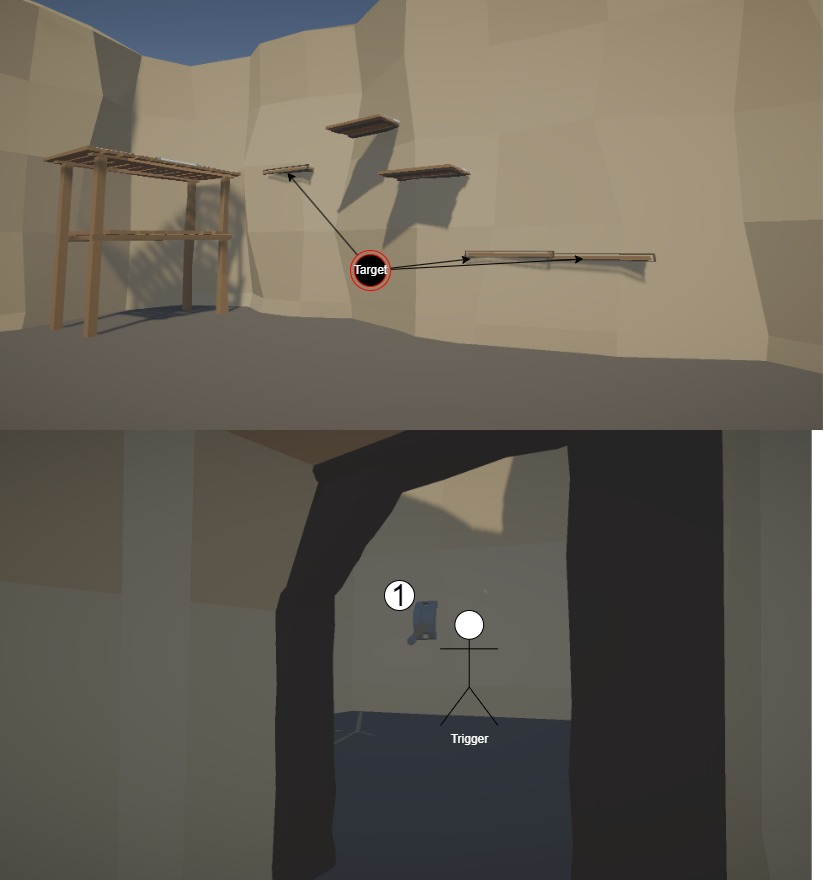
\includegraphics[width=0.8\linewidth]{content/pictures/Raetsel-L01_R02_R01.jpg}
\caption{Element 1 im zweiten Tutorial Raum (Quelle: eigene Darstellung)}
\label{fig:L01_R02_R01}
\end{figure}

Durch eine kleine Öffnung in der Wand kann der Spieler die eingefahrenen Plattformen an der Wand aktivieren. Er muss allerdings am Hebel stehen bleiben, damit dieser nicht wieder einfährt und die Plattformen einfahren lässt. 

Der Spieler benötigt also erneut eine Ich-Version des Chronisten, die den Hebel aktiv hält. Daraus ergibt der Graph aus Abbildung \ref{fig:L01_R01_R01_L}: \nameref{fig:L01_R01_R01_L}:

\begin{figure}[ht]
\centering

\includegraphics[width=00.8\linewidth]{content/pictures/Raetsel-L01_R01_R01_Loesung.jpg}
\caption{Graph zu Element 1 im zweiten Raum (Quelle: eigene Darstellung)}
\label{fig:L01_R01_R01_L_}
\end{figure}

\paragraph{Tutorial, Raum 2, Element 2:}
% \medskip

\begin{figure}[ht]
\centering
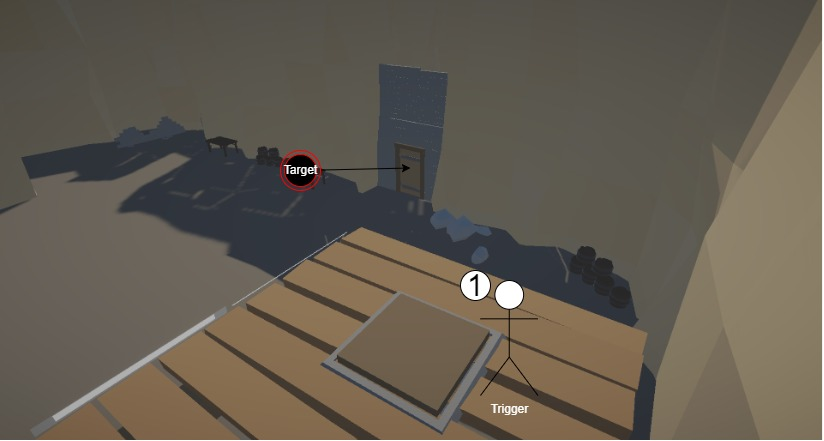
\includegraphics[width=0.8\linewidth]{content/pictures/Raetsel-L01_R02_R02.jpg}
\caption{Element 2 im zweiten Tutorial Raum (Quelle: eigene Darstellung)}
\label{fig:L01_R02_R02}
\end{figure}

Nachdem der Spieler auf das Gerüst geklettert ist, kann er über die Druckplatte die Zieltür öffnen. Durch diese Tür gelangt der Spieler in den nächsten Raum. Daraus ergibt sich folgender Graph in Abbildung \ref{fig:L01_R02_R02_L}: \nameref{fig:L01_R02_R02_L}.

\begin{figure}[ht]
\centering

\includegraphics[width=0.8\linewidth]{content/pictures/Raetsel-L01_R02_R02_Loesung.jpg}
\caption{Lösung Element 2 im zweiten Tutorial Raum (Quelle: eigene Darstellung)}
\label{fig:L01_R02_R02_L}
\end{figure}

Betrachtet man die Elemente des zweiten Raumes als Ganzes, so kann man ihn auf 2 Wege lösen. Zunächst \say{\emph{splittet}} der Spieler entweder in das blaue oder rote Ich des Chronologen. Anschließend \say{\emph{splittet}} er sich in das verbleibende Ich des Chronologen. Mit dem aktuellen Ich betätigt der Spieler den Hebel. Hat der Spieler den Hebel lange genug umgelegt, \say{\emph{mergt}} er auf das Ich vom ersten \say{\emph{Split}} zurück. Mit diesem klettert er die Plattformen an der Wand hoch und aktiviert die Druckplatte. Anschließend \say{\emph{mergt}} der Spieler auf den ursprünglichen Chronologen zurück. Mit diesem kann er, sobald das Ich aus dem ersten \say{\emph{Split}} auf der Druckplatte steht, durch die Tür in den nächsten Raum. Daraus resultiert der Graph aus Abbildung \ref{fig:L01_R02_V01_L}: \nameref{fig:L01_R02_V01_L}.

\begin{figure}[ht]
\centering
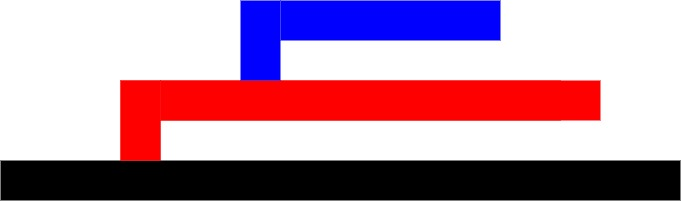
\includegraphics[width=0.8\linewidth]{content/pictures/Raetsel-L01_R02_V01_Loesung.jpg}
\caption{Lösung Variante 1 im zweiten Tutorial Raum (Quelle: eigene Darstellung)}
\label{fig:L01_R02_V01_L}
\end{figure}

Eine andere Möglichkeit wäre es, anstatt des Zweiten \say{\emph{Splits}} vom Roten auf das blaue Ich, ein \say{\emph{Merge}} zurück auf den Chronologen. Anschließend \say{\emph{splittet}} der Spieler auf das verbleibende ich. Nach dem Ersten \say{\emph{Split}} aktiviert der Spieler den Hebel, nach dem Zweiten \say{\emph{Split}} nachdem er zurück \say{\emph{gemergt}} hat, klettert der Spieler auf das Gerüst und öffnet die Tür. Hat der Spieler lange genug gewartet, so kann er auf den Chronologen zurück \say{\emph{mergen}} um in den nächsten Raum zu gelangen. Der dargestellte Graph ist in Abbildung \ref{fig:L01_R02_V02_L}: \nameref{fig:L01_R02_V02_L} ersichtlich.

\begin{figure}[ht]
\centering

\includegraphics[width=0.8\linewidth]{content/pictures/Raetsel-L01_R02_V02_Loesung.jpg}
\caption{Lösung Variante 2 im zweiten Tutorial Raum (Quelle: eigene Darstellung)}
\label{fig:L01_R02_V02_L}
\end{figure}

\paragraph{Tutorial, Raum 3, Element 1:}
% \medskip

\begin{figure}[ht]
\centering
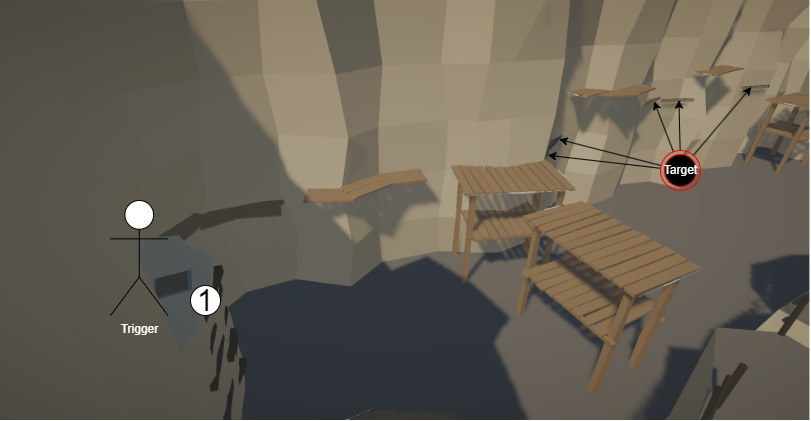
\includegraphics[width=0.8\linewidth]{content/pictures/Raetsel-L01_R03_R01.jpg}
\caption{Element 1 im dritten Tutorial Raum (Quelle: eigene Darstellung)}
\label{fig:L01_R03_R01}
\end{figure}

Über die Druckplatte, mit der Kennnummer 1 in Abbildung \ref{fig:L01_R03_R01}: \nameref{fig:L01_R03_R01} markiert, kann der Spieler die Plattformen an der Wand aktivieren. Über die neu ausgefahrenen Plattformen kann der Spieler mithilfe der statischen Plattformen auf das Gerüst am Ende des Raumes klettern. Für diesen betrachteten Einzelfall ergibt sich derselbe Graph, wie er bereits in Abbildung \ref{fig:L01_R02_R02_L}: \nameref{fig:L01_R02_R02_L} dargestellt wird.

\paragraph{Tutorial, Raum 3, Element 2:}
\medskip

\begin{figure}[ht]
\centering
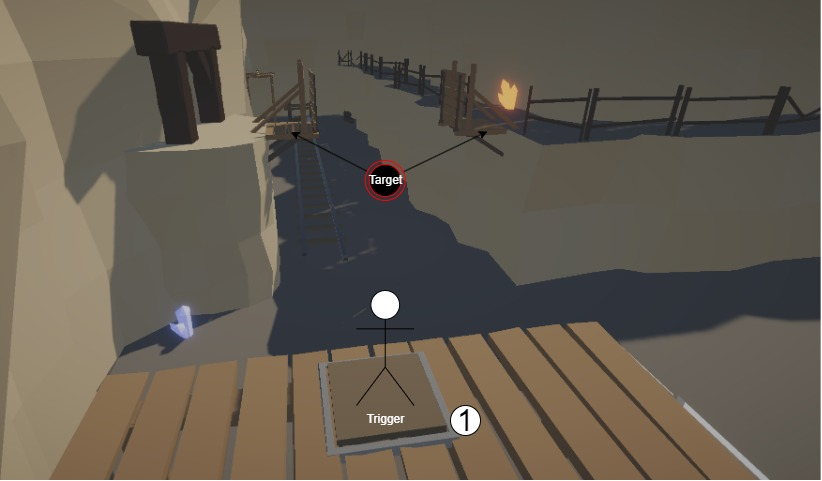
\includegraphics[width=0.8\linewidth]{content/pictures/Raetsel-L01_R03_R02.jpg}
\caption{Element 2 im dritten Tutorial Raum (Quelle: eigene Darstellung)}
\label{fig:L01_R03_R02}
\end{figure}

Damit der Spieler das Level beenden kann, muss er zuletzt die hochgefahrene Brücke überwinden. Über die Druckplatte auf dem Gerüst, auf das er nach erfolgreichem Abschließen von Element 1 kommt, kann der Spieler die Brücke herunterfahren. Dazu benötigt er eine weitere Zeitlinie als Hilfsmittel. Daraus ergibt sich ein Graph, der aussehen kann, wie in Abbildung \ref{fig:L01_R01_R01_L_}: \nameref{fig:L01_R01_R01_L_} oder \ref{fig:L01_R02_R02_L}: \nameref{fig:L01_R02_R02_L}.

Es ist möglich, diesen dritten Raum ebenfalls als Ganzes zu betrachten. Dabei kann sich der Spieler mit dem Chronologen direkt vor der Brücke positionieren oder an der Stelle, bevor er auf das erste Gerüst in Abbildung \ref{fig:L01_R03_R01}: \nameref{fig:L01_R03_R01} springt. Nun \say{\emph{splittet}} der Spieler in eines der möglichen Ichs aus einer anderen Zeitlinie. Er wiederholt den Vorgang erneut und geht nun mit diesem zweiten Ich auf die Druckplatte. Dort wartet er so lange, wie er glaubt, dass er über die Plattformen auf das Gerüst bräuchte. Nachdem er gewartet hat, \say{\emph{mergt}} er auf das als erstes \say{\emph{abgesplitteten}} Ich des Chronologen zurück. Mit diesem kann er, sobald die Plattformen aktiviert wurde, über die Plattform auf das Gerüst klettern und die Druckplatte für die Brücke aktivieren. Der Spieler \say{\emph{mergt}} nun auf den Chronologen zurück und kann über die bald aktivierte Brücke springen. Zudem kann er das Tutorial beenden.
Aus diesem beschriebenen Ablauf ergibt sich folgender Graph, der bereits in Abbildung \ref{fig:L01_R02_V01_L}: \nameref{fig:L01_R02_V01_L} dargestellt wurde.

Hierbei ist es ebenfalls möglich, den Raum im Ganzen auf eine zweite Art zu lösen. Nachdem der Spieler das erste Mal auf sein Ich des Chronologen \say{\emph{gesplittet}} ist und anschließend die Druckplatte von Element 1 aktiv hält, kann er wieder zurück auf den Chronologen \say{\emph{mergen}}. Anschließend kann der Spieler auf das verbleibende Ich des Chronologen \say{\emph{splitten}}. Sobald das bereits \say{\emph{gesplittete}} Ich auf der Druckplatte steht, kann der Spieler mit dem derzeitig \say{\emph{gesplitteten}} Ich über die Plattformen auf die Druckplatte in Element 2 steigen. Nach einem \say{\emph{Merge}} zurück auf den Chronologen kann der Spieler nun über die Brücke gehen. Daraus ergibt sich der Graph, der bereits in Abbildung \ref{fig:L01_R02_V02_L}: \nameref{fig:L01_R02_V02_L} dargestellt wurde.

Im zweiten Level diese Prototypen hat der Spieler zwei weitere Ichs des Chronologen zur Auswahl. Das zweite Level wird Labor genannt und hat einen fertig bestehenden Raum. Dieser wird im Kontext dieser Aufzählung Stromkammer genannt.

\paragraph{Labor, Stromkammer, Element 1:}\label{p:lse1}
% \medskip
\begin{figure}[ht]
\centering
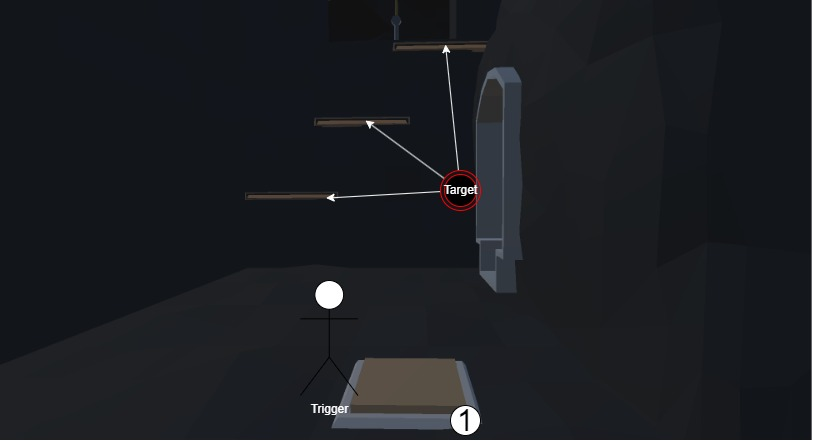
\includegraphics[width=0.8\linewidth]{content/pictures/Raetsel-L02_R01_R01.jpg}
\caption{Element 1 in der Stromkammer (Quelle: eigene Darstellung)}
\label{fig:L02_R01_R01}
\end{figure}

Folgt der Spieler den Stromkabeln in die Stromkammer, so findet er sich in einer kleinen Kammer wieder, in die er zunächst eingesperrt wird. Über eine Druckplatte kann der Spieler Plattformen an der Wand aktivieren, durch welche der Spieler aus der Kammer in die große Grotte gelangt (vgl. Abbildung \ref{fig:L02_R01_R01}).
Dazu benötigt er ein Ich des Chronologen, in welchen der Spieler \say{\emph{splittet}} um im Anschluss auf den Chronologen zurück zu  \say{\emph{mergen}}. Daraus ergibt sich wiederum ein Graph, der ähnlich zu Abbildung \ref{fig:L01_R01_R01_L_}: \nameref{fig:L01_R01_R01_L_} oder \ref{fig:L01_R02_R02_L}: \nameref{fig:L01_R02_R02_L} aussehen kann.

\paragraph{Labor, Stromkammer, Element 2:}\label{p:lse2}

\begin{figure}[ht]
\centering
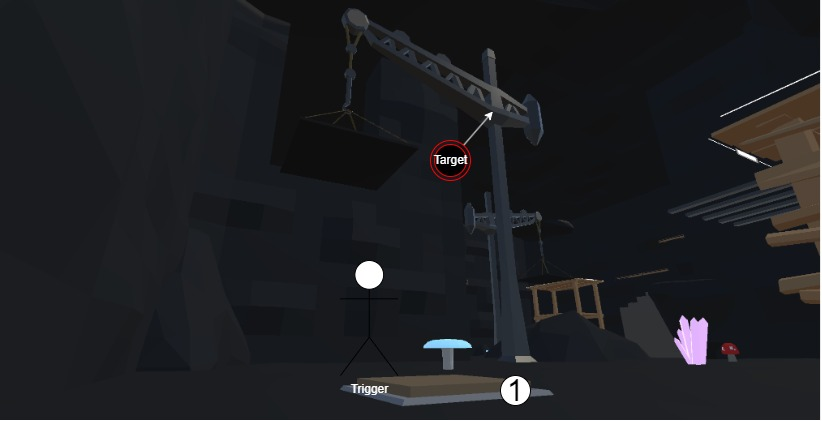
\includegraphics[width=0.8\linewidth]{content/pictures/Raetsel-L02_R01_R02.jpg}
\caption{Element 2 in der Stromkammer (Quelle: eigene Darstellung)}
\label{fig:L02_R01_R02}
\end{figure}

Sobald der Spieler aus dem Eingangsraum herausgefunden hat, kann er mithilfe des Krans erneut wieder in die Kammer gehen. Außerdem kann der Spieler über den ersten Kran mit dem zweiten Kran in Kombination auf das Gerüst am Ende der Grotte gelangen. Um das zu erreichen, benötigt er allerdings mehrere Komponenten als ausschließlich den Kran. Über die Druckplatte kann der Spieler den Kran aktivieren. Daraus erfolgt derselbe Graph, der ähnlich wie Abbildung\ref{fig:L01_R01_R01_L_}: \nameref{fig:L01_R01_R01_L_} oder \ref{fig:L01_R02_R02_L}: \nameref{fig:L01_R02_R02_L} aussehen kann.

\paragraph{Labor, Stromkammer, Element 3:}\label{p:lse3}

\begin{figure}[ht]
\centering
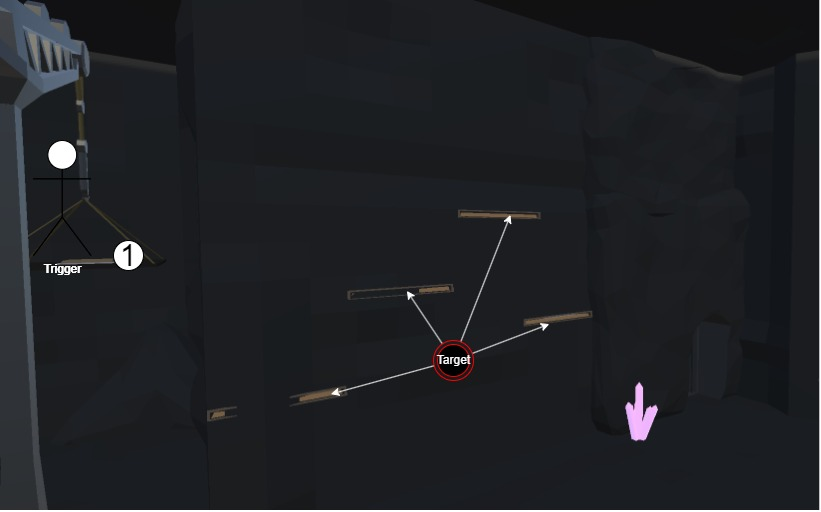
\includegraphics[width=0.8\linewidth]{content/pictures/Raetsel-L02_R01_R03.jpg}
\caption{Element 3 in der Stromkammer (Quelle: eigene Darstellung)}
\label{fig:L02_R01_R03}
\end{figure}

Die Druckplatte auf der Kranplattform aktiviert weitere Plattformen an der Wand. Diese Plattformen sind wichtig, um letztlich an den Stromansteller zu gelangen. Um hierbei nicht mit dem Chronologen die Druckplatte zu aktivieren, wird wiederum ein weiteres Ich des Chronologen benötigt. 

Im Folgenden wird kein Abbild des Graphen dargestellt, da die beiden Kräne zu einem Mechanismus gehören, welcher nur im Ganzen gelöst werden kann. Später wird darauf separat eingegangen.

\paragraph{Labor, Stromkammer, Element 4:}\label{p:lse4}

\begin{figure}[ht]
\centering
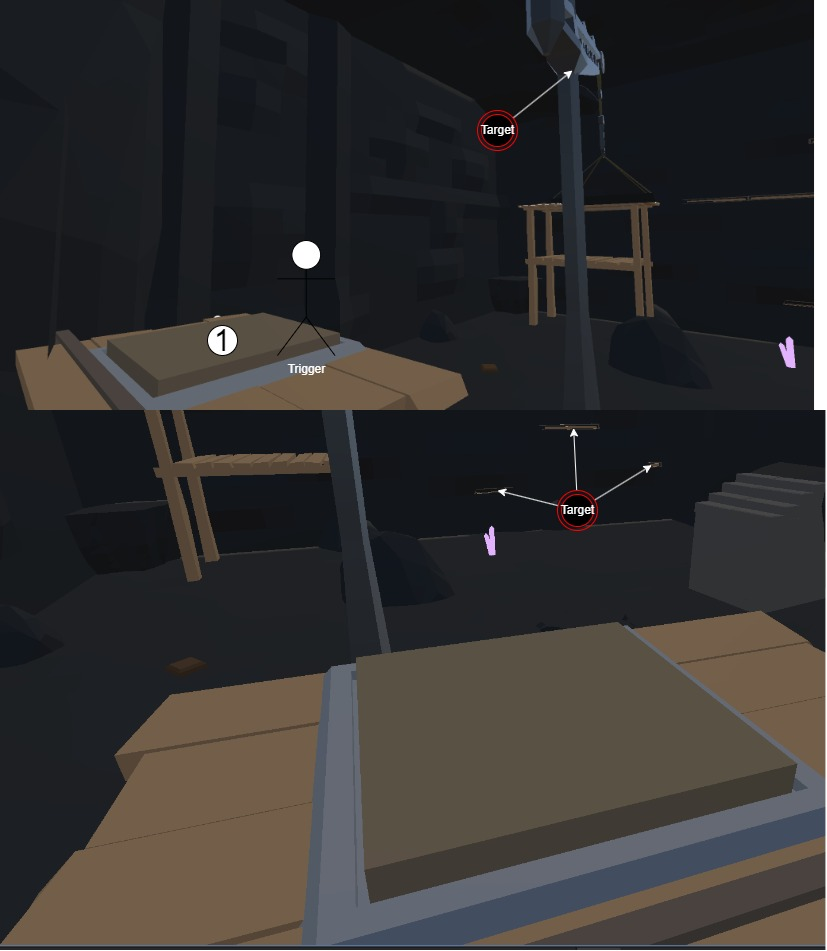
\includegraphics[width=0.8\linewidth]{content/pictures/Raetsel-L02_R01_R04.jpg}
\caption{Element 4 in der Stromkammer (Quelle: eigene Darstellung)}
\label{fig:L02_R01_R04}
\end{figure}

Durch die Druckplatte in \nameref{p:lse3}, werden an der Wand nun die Plattformen aktiv und der Spieler kann auf eine neu erschienene Druckplatte steigen. Diese Druckplatte aktiviert zum einen den zweiten Kran und zum anderen Druckplatten an der Wand neben dem Hochstand, der ein Zwischenziel darstellt. Um auf diese Druckplatte zu gelangen, benötigt der Spieler ein weiteres Ich des Chronologen, um mit diesem den zweiten Kran zu aktivieren. Über den zweiten Kran gelangt der Spieler nun auf diesen Hochstand.

Im Anschluss werden die Elemente \nameref{p:lse2} bis \nameref{p:lse4} aus der Stromkammer benutzt, um den daraus resultierenden Graphen als ein ganzes zusammenzusetzen.

Wie erwähnt muss der Spieler zum einen den Kran in Bewegung setzen, damit er an die Schnittstelle der zwei Kräne gelangt. Der zweite Kran muss nun auch aktiviert werden, das geschieht zum einen durch die Druckplatte auf dem ersten Kran aus Element \nameref{p:lse3} und zum anderen durch die frei werdende Druckplatte in Element \nameref{p:lse4}. Der zweite Kran fährt nach der Aktivierung zur Schnittstelle der zwei Kräne und anschließend wieder zurück zum Hochstand. Der Spieler bräuchte für diesen Zwischenschritt insgesamt drei weitere Ichs des Chronologen. Der Graph, der diesen Weg ebnen lässt, sieht folgendermaßen aus. Er wird in Abbildung \ref{fig:L02_E02_04_L01}: \nameref{fig:L02_E02_04_L01} gezeigt.

\begin{figure}[ht]
\centering
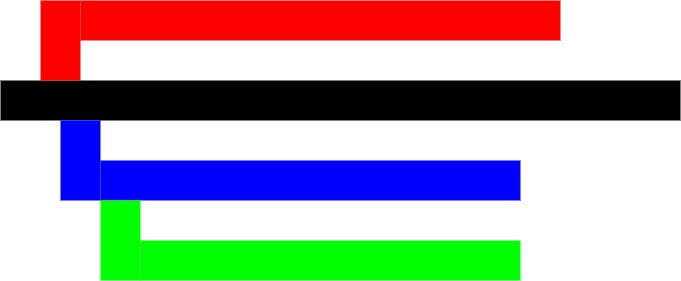
\includegraphics[width=0.8\linewidth]{content/pictures/Raetsel-L02_E02_4_V01_Loesung}
\caption{Lösungsweg gesamt Element 2 bis 4 (Quelle: eigene Darstellung)}
\label{fig:L02_E02_04_L01}
\end{figure}

Die rote Zeitlinie repräsentiert das Ich des Chronologen, welches auf die Druckplatte steigt, welche den Kran in Bewegung setzt. Er muss die Druckplatte so lange aktiv halten, bis der Spieler vom ersten auf den zweiten Kran gesprungen ist. Der Spieler \say{\emph{mergt}} in den Chronologen zurück, um auf den zweiten Kran zu gelangen. Anschließend \say{\emph{splittet}} der Spieler in die blaue Zeitlinie, von dort aus in die Grüne. Mit dem Chronologen der grünen Zeitlinie stellt sich der Spieler auf die Druckplatte der Kranplattform. Diese öffnet die Plattformen an der Wand von Abbildung \ref{fig:L02_R01_R03}: \nameref{fig:L02_R01_R03}. Nachdem er lange genug gewartet hat, \say{\emph{mergt}} der Spieler zurück auf den Chronologen der blauen Zeitlinie. Mit diesem Ich des Chronologen steigt der Spieler nun auf die geöffnete Druckplatte aus Abbildung \ref{fig:L02_R01_R03}: \nameref{fig:L02_R01_R03}. Dadurch setzt sich der zweite Kran in Bewegung und fährt zur Schnittstelle und wieder zurück. Anschließend \say{\emph{mergt}} der Spieler auf den eigentlichen Chronologen zurück und springt über den aktivierten zweiten Kran auf das Gerüst um das Zwischenziel zu erreichen.

\paragraph{Labor, Stromkammer, Element 5:}\label{p:lse5}

\begin{figure}[ht]
\centering
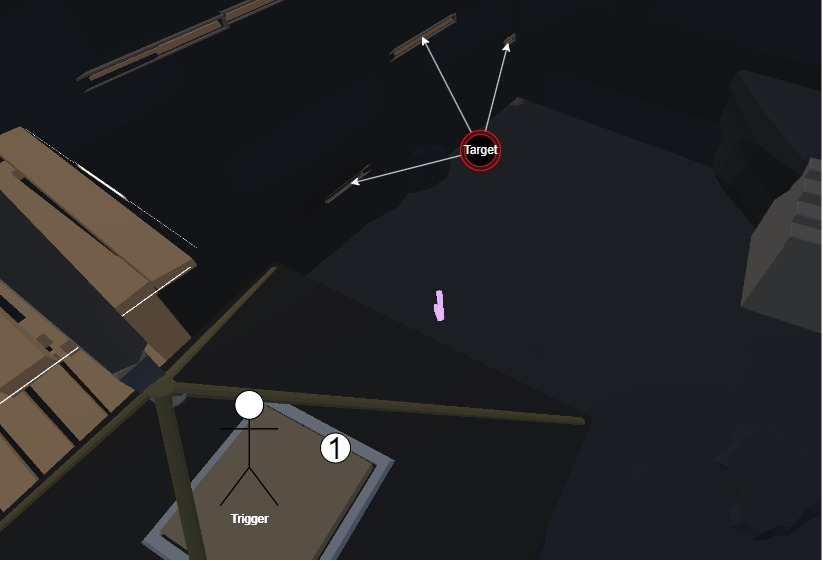
\includegraphics[width=0.8\linewidth]{content/pictures/Raetsel-L02_R01_R05.jpg}
\caption{Element 5 in der Stromkammer (Quelle: eigene Darstellung)}
\label{fig:L02_R01_R05}
\end{figure}

Wie in Abbildung \ref{fig:L02_R01_R04}: \nameref{fig:L02_R01_R04} bereits gezeigt, öffnet ebenfalls die Druckplatte auf dem zweiten Kran die unteren drei Plattformen, die in Abbildung \ref{fig:L02_R01_R05}: \nameref{fig:L02_R01_R05} gekennzeichnet sind. Eine der ausfahrbaren Plattformen enthält eine Druckplatte, welche das letzte Stück des Weges aktiviert. Hierfür wird wieder ein Ich des Chronologen benötigt. Möglich ist es auch, dass erzeugten Zeitlinien von oben noch aktiv sind, dann wären die Plattformen bereits ausgefahren. Wenn man nicht von diesem Fall ausgeht, sieht der Graph aus wie in Abbildung \ref{fig:L01_R01_R01_L_}: \nameref{fig:L01_R01_R01_L_} oder \ref{fig:L01_R02_R02_L}: \nameref{fig:L01_R02_R02_L} bereits dargestellt.

\paragraph{Labor, Stromkammer, Element 6:}\label{p:lse6}

\begin{figure}[ht]
\centering
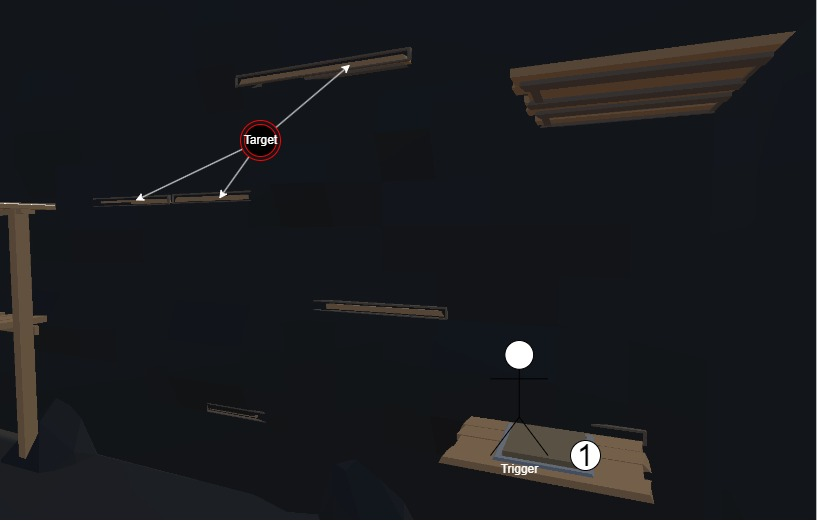
\includegraphics[width=0.8\linewidth]{content/pictures/Raetsel-L02_R01_R06.jpg}
\caption{Element 6 in der Stromkammer (Quelle: eigene Darstellung)}
\label{fig:L02_R01_R06}
\end{figure}

Die Druckplatte aus Abbildung \ref{fig:L02_R01_R06}: \nameref{fig:L02_R01_R06} öffnet nun die letzten Plattformen, um in den Raum zu gelangen, indem der Strom angeschlossen werden kann. Hierfür wird ebenfalls ein weiteres Ich des Chronologen benötigt.

Fasst man die Schritte aus Element \nameref{p:lse5} und \nameref{p:lse6} zusammen, so würde das einem Graphen aus Abbildung 14 oder 15 gleichen. Der Spieler muss in ein Ich des Chronologen \say{\emph{splitten}} um über die Druckplatte auf der Kranplattform die Plattformen an der Wand aktivieren. Das wären in Abbildung \ref{fig:L01_R02_V01_L}: \nameref{fig:L01_R02_V01_L} und \ref{fig:L01_R02_V02_L}: \nameref{fig:L01_R02_V02_L} jeweils die blaue Zeitlinie. Anschließend \say{\emph{mergt}} der Spieler wie in Abbildung \ref{fig:L01_R02_V02_L}: \nameref{fig:L01_R02_V02_L} zurück auf den Chronologen und \say{\emph{splittet}} in ein weiteres Ich. Denkbar ist es auch, dass der Spieler wie in Abbildung \ref{fig:L01_R02_V01_L}: \nameref{fig:L01_R02_V01_L} auf die rote Zeitlinie zurück \say{\emph{mergt}} um anschließend die geöffnete Druckplatte zu aktivieren. Nachdem diese Plattform eine Zeit aktiv war, \say{\emph{mergt}} der Spieler zurück auf den Chronologen und gelangt so in den Raum, in dem er den Strom einschalten kann.

\paragraph{Labor, Stromkammer, Element 7:}\label{p:lse7}

\begin{figure}[ht]
\centering
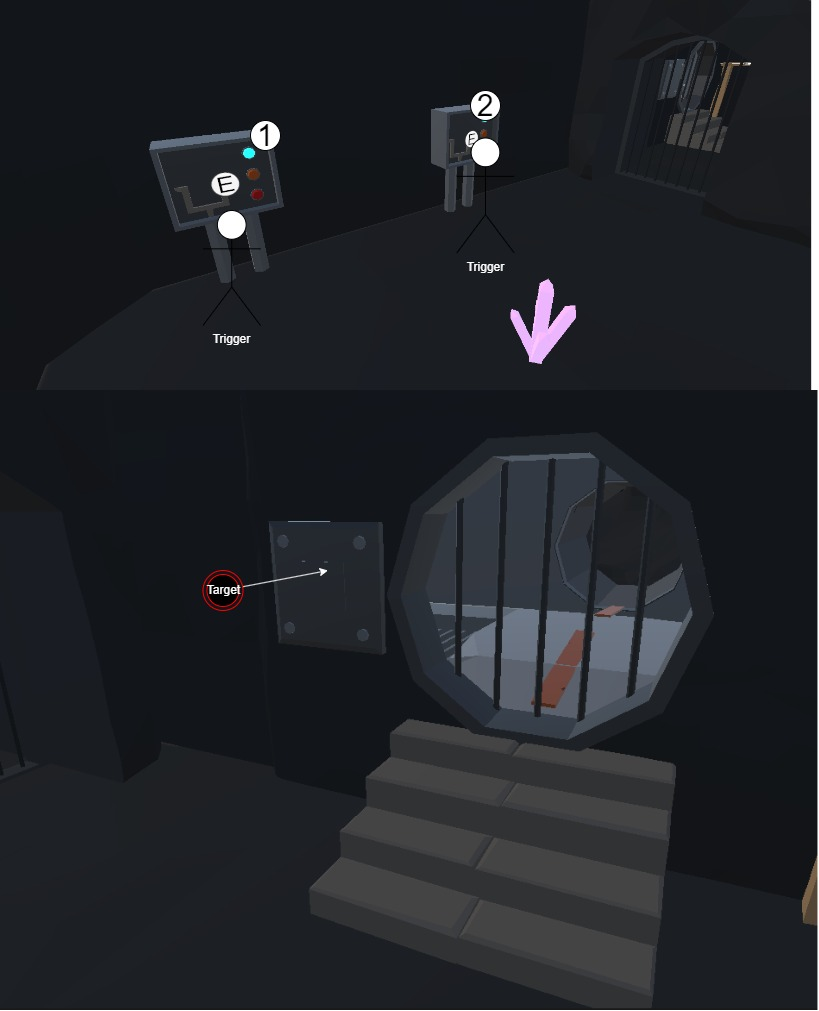
\includegraphics[width=0.8\linewidth]{content/pictures/Raetsel-L02_R01_R07.jpg}
\caption{Element 7 in der Stromkammer (Quelle: eigene Darstellung)}
\label{fig:L02_R01_R07}
\end{figure}

Angekommen in der Stromschaltzentrale, muss der Spieler über die 2 Stromschalter den Strom für das Labor anstellen. Hierzu muss der Spieler zunächst in ein weiteres Ich des Chronologen \say{\emph{splitten}} damit nach einem folgenden \say{\emph{Merge}} beide Hebel der Aktivatoren betätigt werden können. Ein Graph, der diese Interaktion beschreibt, ist in Abbildung \ref{fig:L01_R01_R01_L_}: \nameref{fig:L01_R01_R01_L_} oder \ref{fig:L01_R02_R02_L}: \nameref{fig:L01_R02_R02_L} zu finden. Nachdem der Strom angestellt wurde, gelangt der Spieler wieder in die Grotte zurück.

Es fehlt jetzt nur noch die Öffnung des Ausgangs.

\paragraph{Labor, Stromkammer, Element 8:}\label{p:lse8}

\begin{figure}[ht]
\centering
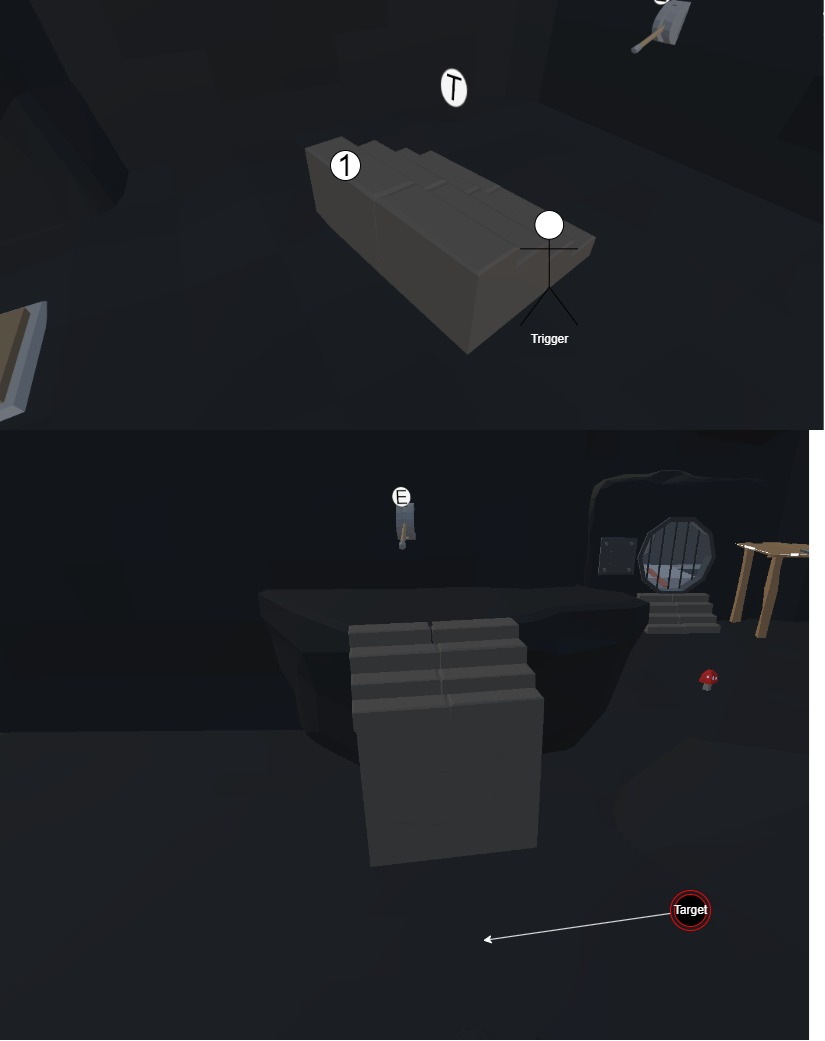
\includegraphics[width=0.8\linewidth]{content/pictures/Raetsel-L02_R01_R08.jpg}
\caption{Element 8 in der Stromkammer (Quelle: eigene Darstellung)}
\label{fig:L02_R01_R08}
\end{figure}

Auf dem Felsen an der Wand des Raumes, in dem der Spieler zuvor den Strom aktiviert hat, befindet sich ein Hebel, der das Tor zum Ausgang der Grotte öffnet. Dieser Hebel benötigt Strom. Um auf den Felsen zu kommen, benötigt der Spieler einen Teil der Treppe, um von diesem auf den bestehenden Teil der Treppe zu springen. Das fehlende Stück befindet sich in der Eingangskammer, aus der der Spieler am Anfang über die Plattformen herausgeklettert ist. Zunächst muss der Spieler wieder in diese Kammer. Die Kammer kann über einen zweiten Weg geöffnet werden. Das Portal kann über die in Abbildung \ref{fig:L02_R01_R10}: \nameref{fig:L02_R01_R10} gekennzeichneten Hebel geöffnet werden.

\paragraph{Labor, Stromkammer, Element 9:}\label{p:lse9}

\begin{figure}[ht]
\centering
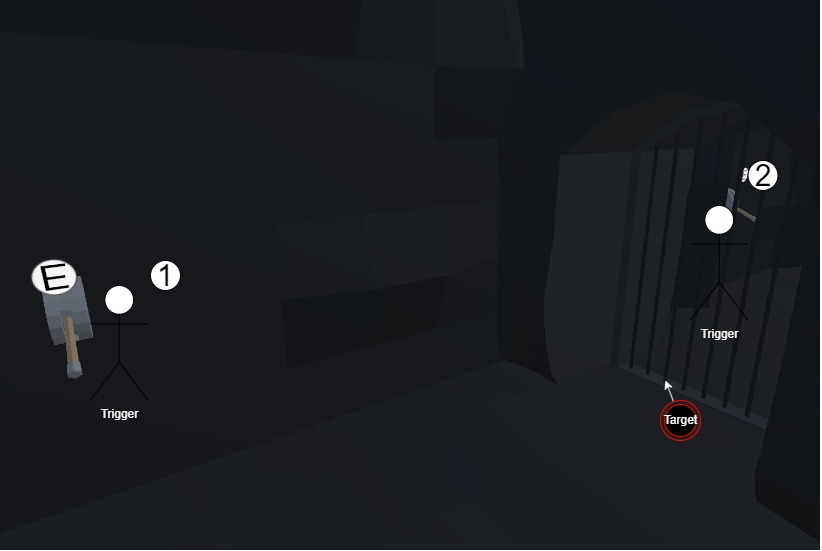
\includegraphics[width=0.8\linewidth]{content/pictures/Raetsel-L02_R01_R10.jpg}
\caption{Element 9 in der Stromkammer (Quelle: eigene Darstellung)}
\label{fig:L02_R01_R10}
\end{figure}

Der Spieler muss nun mit einem Ich des Chronologen in die Kammer zurück, um den Hebel in der Kammer umzulegen. Dafür benötigt der Spieler erneut ein Ich des Chronologen, da der Kran hierfür aktiviert werden muss. Vom Hochstand, der neben dem Portal am Ausgang steht, kann der Spieler auf die Plattform des Kranes springen. Der Kran fährt eine Runde von der Öffnung an der Wand zum Hochstand und wieder zurück, ehe er weiter zur Schnittstelle mit dem zweiten Kran fährt. So kann der Spieler nun mit einer \say{\emph{gesplitteten}} Version des Chronologen in die Kammer gelangen. Auf der Außenseite der Kammer benötigt der Spieler ebenfalls ein weiteres Ich. Sobald die beiden Hebel gleichzeitig aktiviert wurden, öffnet sich das Portal und der Spieler kann die darin liegende Treppe heraustragen. Diese muss er, wie in Abbildung \ref{fig:L02_R01_R08}: \nameref{fig:L02_R01_R08} gezeigt, vor die bestehende Treppe legen, damit der Spieler nun auf den Felsen springen kann. Der dabei entstehende Graph wird in Abbildung \ref{fig:L02_E08_9_V01}: \nameref{fig:L02_E08_9_V01} gezeigt.

\begin{figure}[ht]
\centering
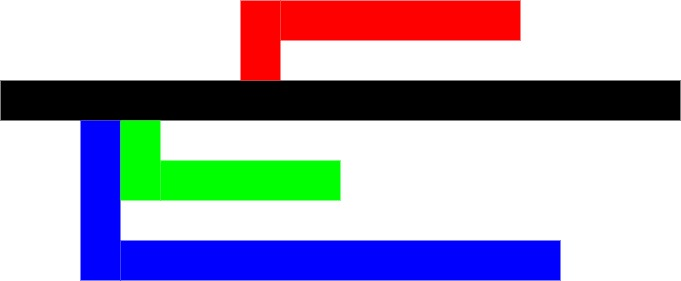
\includegraphics[width=1\linewidth]{content/pictures/Raetsel-L02_E08_9_V01_Loesung.jpg}
\caption{Lösungsweg gesamt Element 8 bis 9 (Quelle: eigene Darstellung)}
\label{fig:L02_E08_9_V01}
\end{figure}

Das grüne Ich des Chronologen aktiviert den Kran, sodass das blaue Ich über den Kran in die Kammer gelangt. In der Kammer angelangt, aktiviert der Spieler den inneren Hebel. Nach einem \say{\emph{Merge}} zurück auf den Chronologen, \say{\emph{splittet}} er in das rote Ich und öffnet mit ihm gleichzeitig mit dem blauen Ich den zweiten Hebel und damit das Portal. Anschließend \say{\emph{mergt}} er auf den Chronologen zurück, um durch das offene Portal in die Kammer zu gelangen. Anschließend trägt er die Treppe an die in Abbildung \ref{fig:L02_R01_R08}: \nameref{fig:L02_R01_R08} gekennzeichnete Stelle.

\paragraph{Labor, Stromkammer, Element 10:}\label{p:lse10}

\begin{figure}[ht]
\centering
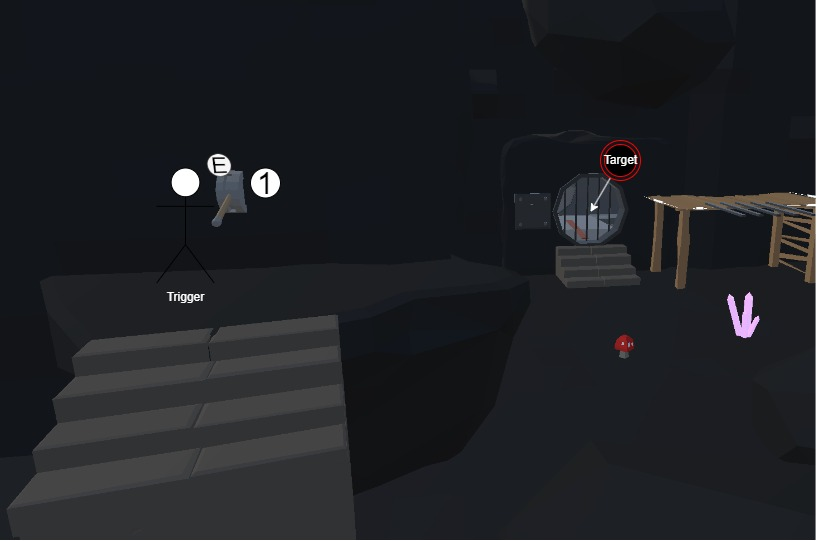
\includegraphics[width=1\linewidth]{content/pictures/Raetsel-L02_R01_R09.jpg}
\caption{Element 10 in der Stromkammer (Quelle: eigene Darstellung)}
\label{fig:L02_R01_R09}
\end{figure}

Im letzten Schritt muss der Spieler über die Treppe auf den Felsen springen und kann durch den Hebel das Portal am Ausgang öffnen. Der Hebel besitzt nun Strom und das Portal kann geöffnet werden. So gelangt der Spieler zurück zum Eingang des Labors.

\subsubsection{Konzipierte Rätsel}

Im Anschluss folgen nun die konzipierten Rätsel, diese kommenden Rätsel werden allesamt im zweiten Level des Prototyps zu finden sein. Den ersten Raum, um den es gleich gehen wird, wird Laboreingang genannt und wurde in der Szene umgesetzt, allerdings besitzt dieser Raum noch keine  Interaktivität.

Zuerst wird auf die einzelnen Elemente des Laboreingangs eingegangen. Anschließend wird die Lösung mitsamt einem daraus entstehenden Graphen gezeigt.

\paragraph{Labor, Laboreingang, Element 1:}\label{p:lle1}

\begin{figure}[ht]
\centering
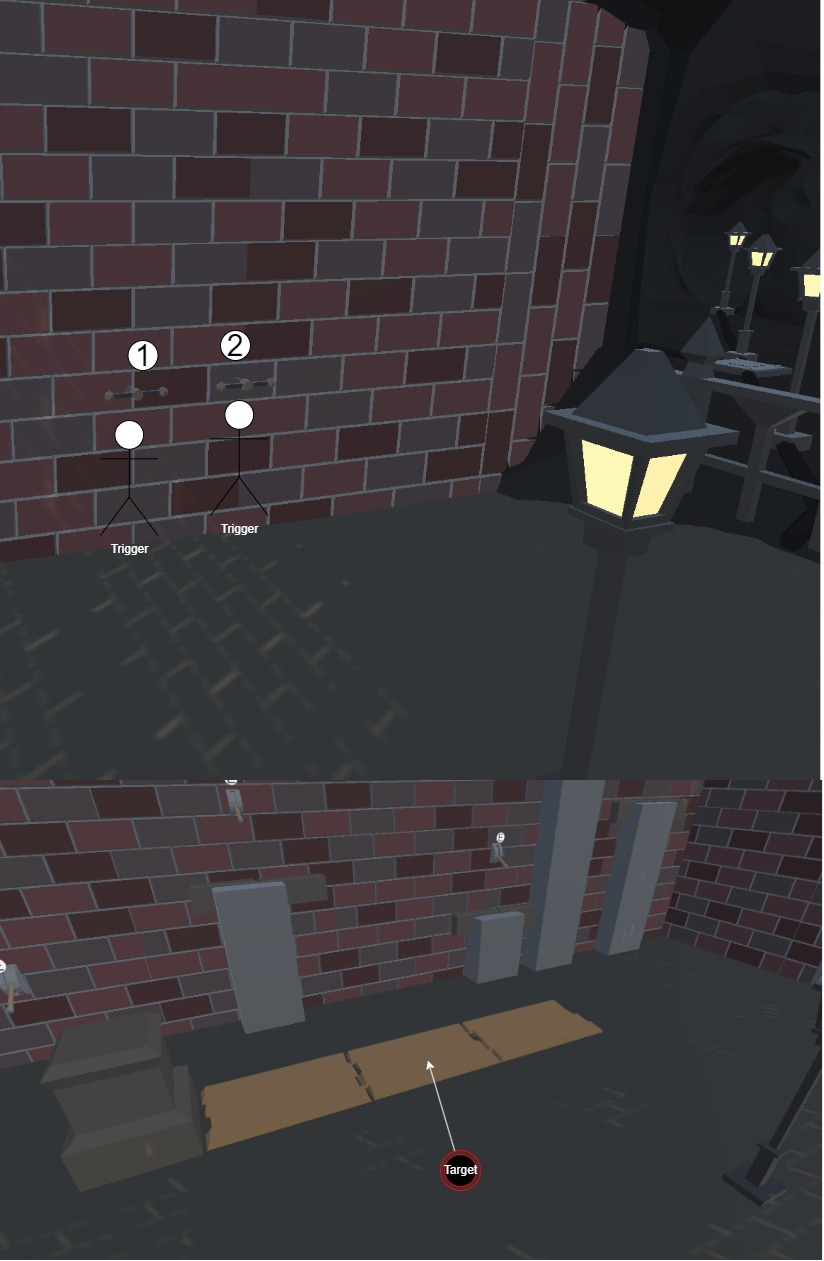
\includegraphics[width=0.8\linewidth]{content/pictures/Raetsel-L02_R02_R01.jpg}
\caption{Element 1 im Laboreingang (Quelle: eigene Darstellung)}
\label{fig:L02_R02_R01}
\end{figure}

Wie in Abbildung \ref{fig:L02_R02_R01}: \nameref{fig:L02_R02_R01} besitzt der Eingang eine bewegbare Plattform, die sich zwischen der Rückwand des Einganges und dem anliegenden Begrenzer bewegen kann. Zudem ist es möglich, diese Plattform auch auf die Höhe des Begrenzers anzuheben. Der Spieler hat dazu zwei Ventile zur Auswahl. Mit dem einen Ventil kann der Spieler die Plattform an die Wand oder wieder zurückfahren. Mit dem anderen Ventil kann er die Plattform auf die Höhe des Begrenzers oder wieder auf den Boden fahren lassen. Das ermöglicht einem \say{\emph{gesplitteten}} Ich des Chronologen die Stützen an der Wand vor die Hebel zu stellen.

Durch die bewegende Plattform kann der Spieler jetzt Stützen aufeinanderstellen. Sobald der Chronologe ein Objekt trägt, kann dieser nicht springen.

\paragraph{Labor, Laboreingang, Element 2:}\label{p:lle2}

\begin{figure}[ht]
\centering
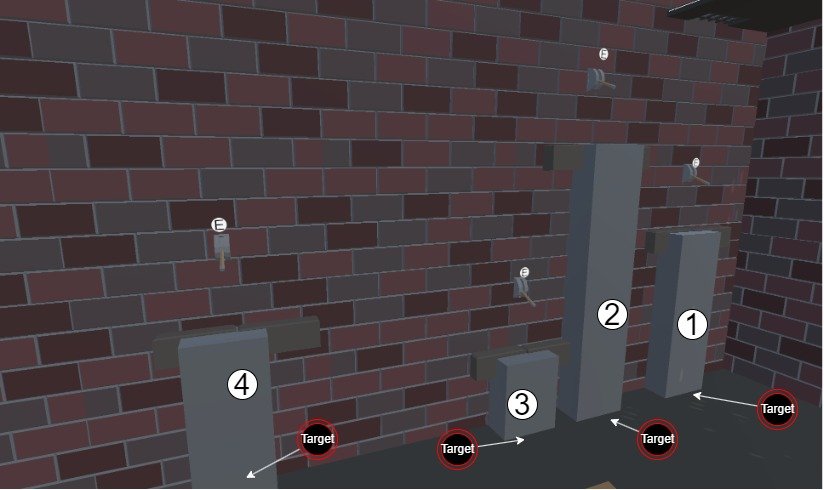
\includegraphics[width=0.8\linewidth]{content/pictures/Raetsel-L02_R02_R02.jpg}
\caption{Element 2 im Laboreingang (Quelle: eigene Darstellung)}
\label{fig:L02_R02_R02}
\end{figure}

Wie eben dargestellt und in Abbildung \ref{fig:L02_R02_R02}: \nameref{fig:L02_R02_R02} zu sehen, sind an einer der Seiten des Einganges Hebel an der Wand befestigt. Jeweils unter den einzelnen Hebeln ist ein kleiner Vorsprung, der dem Spieler anzeigen soll, an welche Stelle die Stütze gestellt werden muss. Der Spieler hat die Möglichkeit, auf die Stützen 4 und 2 zu klettern. Durch die Hilfe zwei weiterer Chronologen kann der Spieler nun mit einem Ich die Stützen in der richtigen Reihenfolge aufzustellen, damit ein weiteres Ich zu den Hebeln klettern kann.

\paragraph{Labor, Laboreingang, Element 3:}\label{p:lle3}

\begin{figure}[ht]
\centering
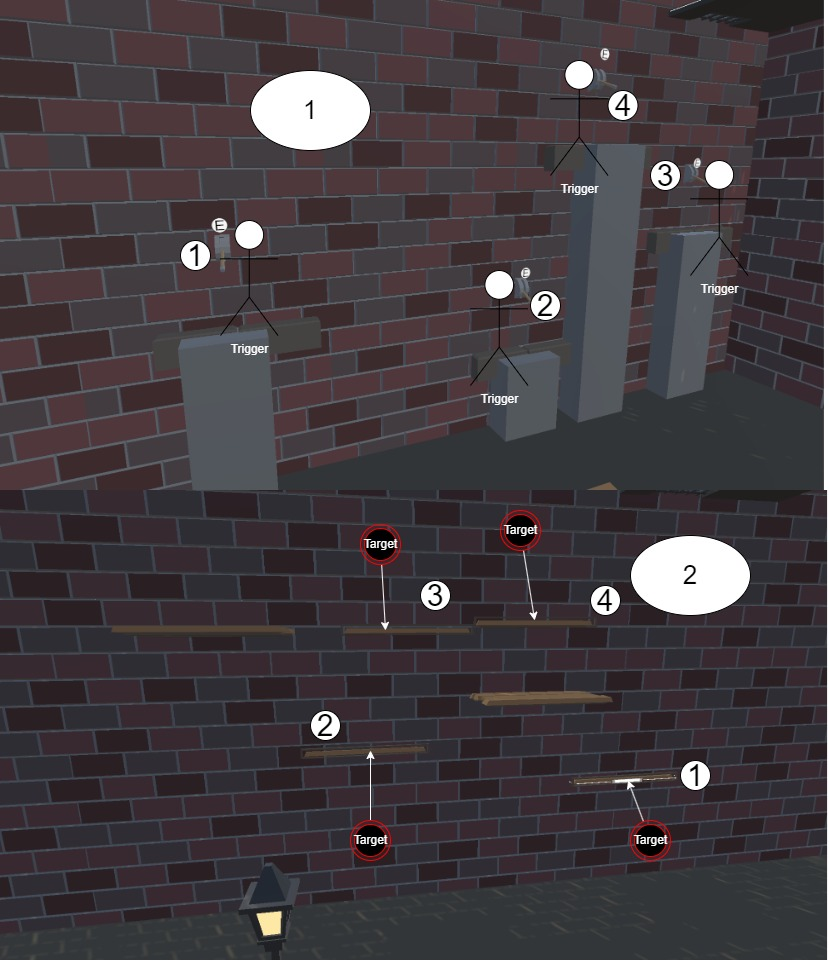
\includegraphics[width=0.8\linewidth]{content/pictures/Raetsel-L02_R02_R03.jpg}
\caption{Element 3 im Laboreingang (Quelle: eigene Darstellung)}
\label{fig:L02_R02_R03}
\end{figure}

Die Hebel, in Abbildung \ref{fig:L02_R02_R03}: \nameref{fig:L02_R02_R03}, an der Wand mit der Markierung 1 öffnen jeweils eine Plattform an der gegenüberliegenden Wand, welche mit einer 2 markiert ist. Ein Ich des Chronologen muss nun, wie in Element 2 angesprochen, die Hebel in der richtigen Reihenfolge betätigen. Dadurch kann ein weiteres Ich auf der gegenüberliegenden Seite über die ausgefahrenen Plattformen in die nächste Etage des Einganges klettern kann. 

\paragraph{Labor, Laboreingang, Element 4:}\label{p:lle4}

\begin{figure}[ht]
\centering
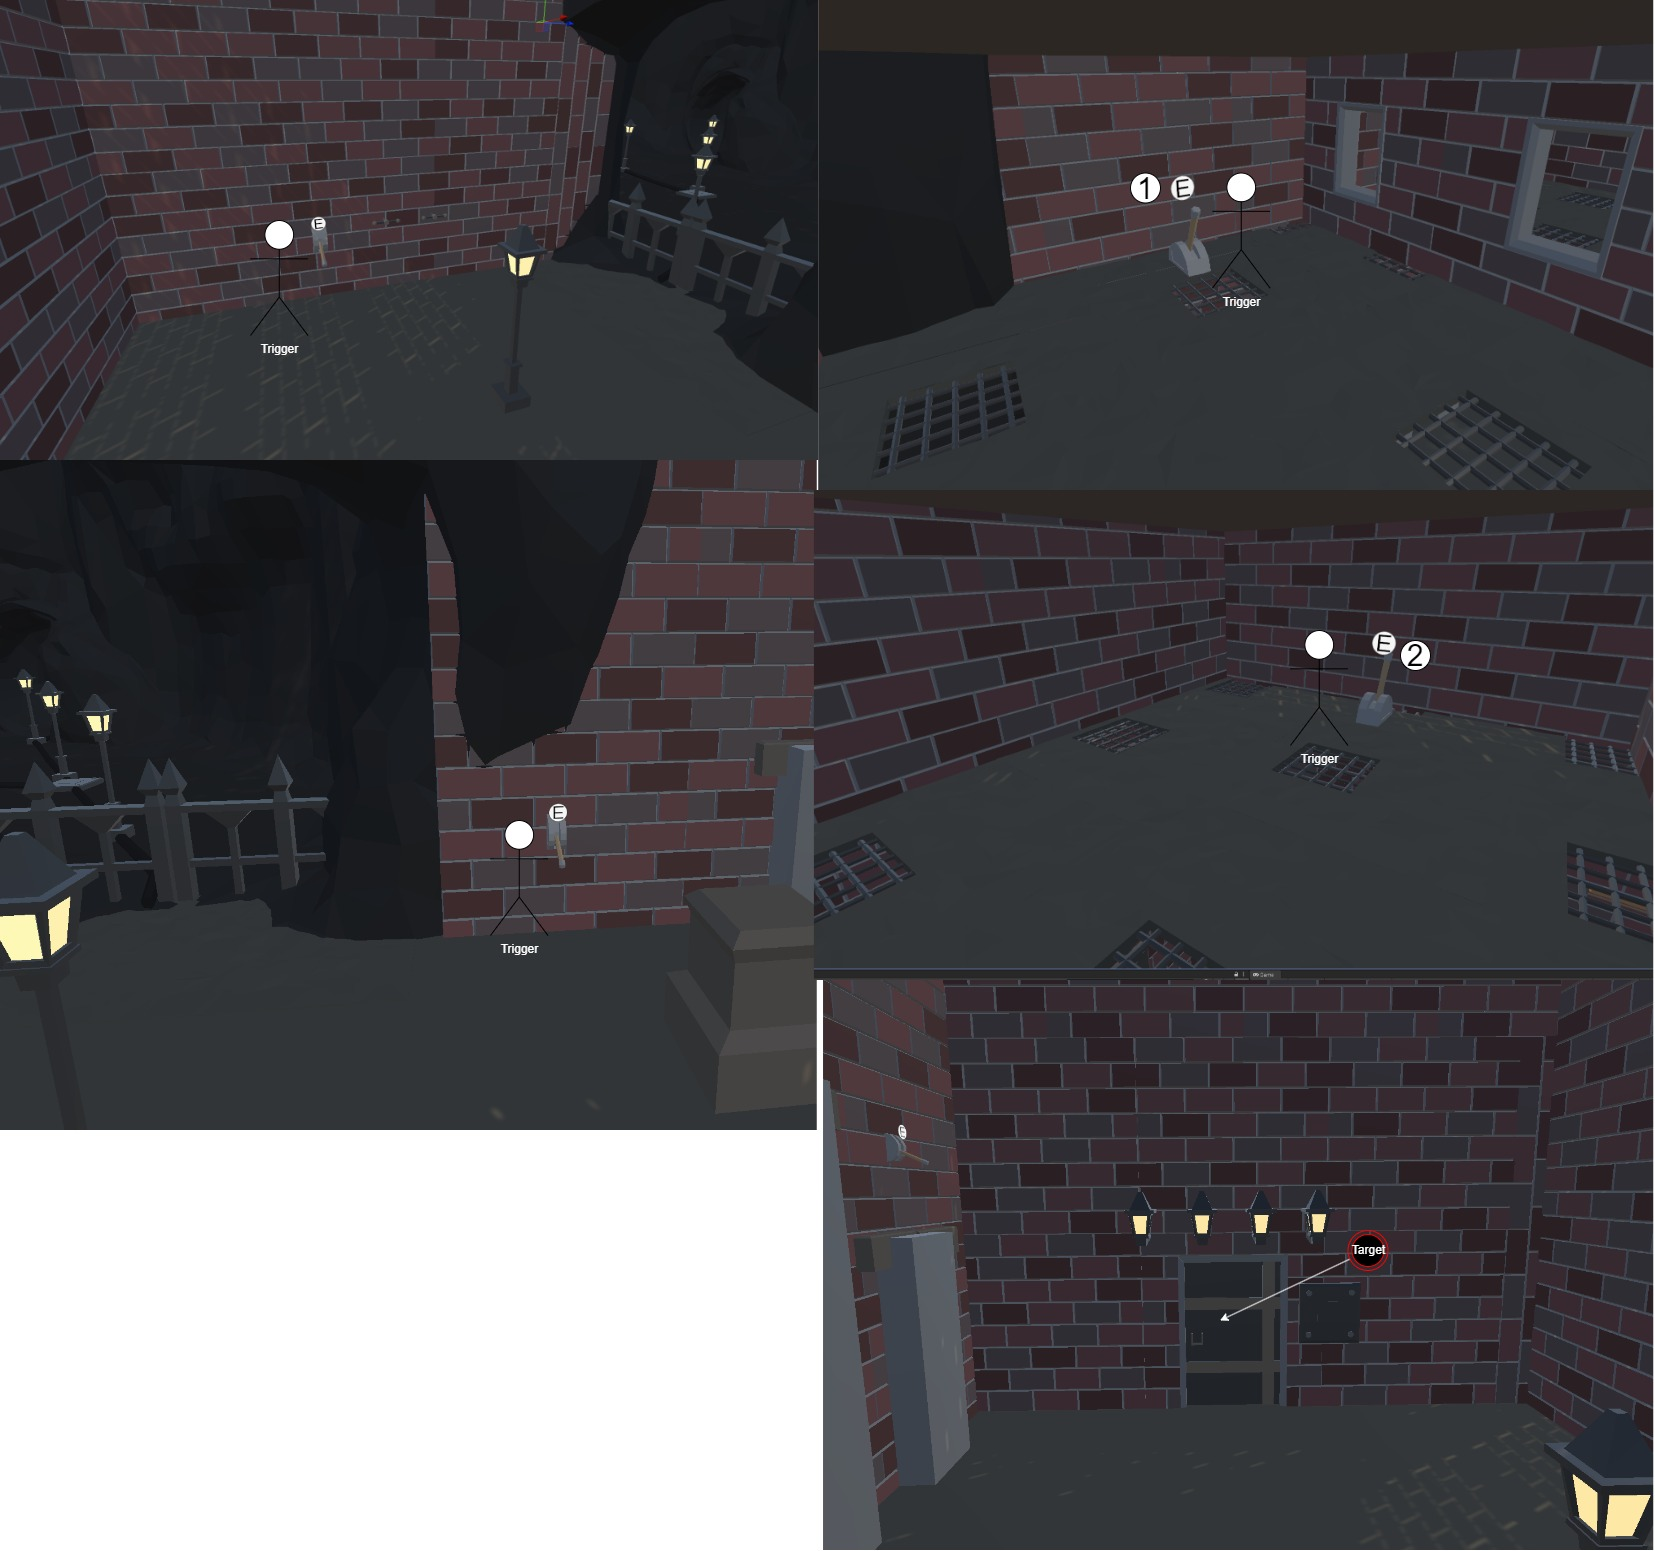
\includegraphics[width=0.8\linewidth]{content/pictures/Raetsel-L02_R02_R04.jpg}
\caption{Element 4 im Laboreingang (Quelle: eigene Darstellung)}
\label{fig:L02_R02_R04}
\end{figure}

Das Ich, das über die Hebel die Plattformen auf der gegenüberliegenden Wand betätigt, kann ebenfalls auf die zweite Etage des Eingangs klettern. Auf der oberen Etage befinden sich zwei von vier Hebeln, die aktiviert werden müssen, damit der Spieler in das Labor gehen kann. Außerdem befinden sich jeweils neben dem Eingang in diesen Eingangsraum zwei weitere Hebel, die der Spieler aktivieren muss. Über der schweren Eisentür befinden sich vier Lampen, die die Aktivität der vier Hebel anzeigt (Licht an/ aktiv – Licht aus/ inaktiv). Wird ein Hebel betätigt, so leuchtet die jeweilige Lampe. Sobald alle vier Hebel gleichzeitig aktiviert wurden, kann der Spieler durch die Tür gehen. Die Hebel müssen allerdings aktiviert bleiben, bewegt sich ein \say{\emph{gesplittetes}} Ich vom Hebel weg, so schließt sich die Tür (vgl. Abbildung \ref{fig:L02_R02_R04}: \nameref{fig:L02_R02_R04}).

Da diese vier Elemente miteinander in einer abgestimmten Reihenfolge betätigt werden müssen, ergibt sich ein in Abbildung \ref{fig:L02_R02_E01_4_V01}: \nameref{fig:L02_R02_E01_4_V01} abgebildeter Graph.

\begin{figure}[ht]
\centering
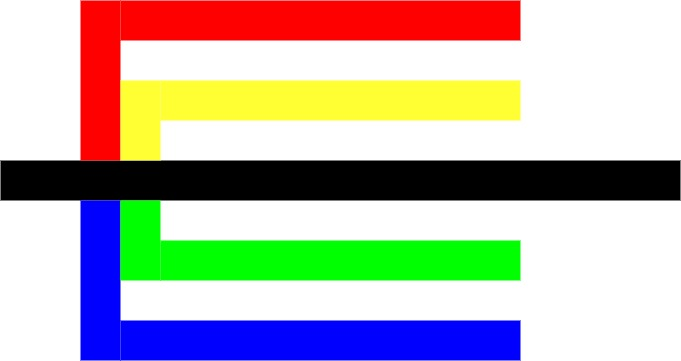
\includegraphics[width=0.8\linewidth]{content/pictures/Raetsel-L02_R02_E01_4_V01_Loesung}
\caption{Lösungsweg gesamt Element 1 bis 4 (Quelle: eigene Darstellung)}
\label{fig:L02_R02_E01_4_V01}
\end{figure}

Zuerst muss der Spieler in das rote Ich des Chronologen \say{\emph{splitten}}. Durch diesen kann der Spieler die am Boden liegende Plattform bewegen. Der Spieler muss jetzt für einen späteren Zeitpunkt die Plattform jeweils so positionieren, dass er die Stützen für ein weiteres Ich richtig positionieren kann. Bevor der Spieler \say{\emph{zurückmergt}} betätigt er den Hebel, der neben den zwei Ventilen zu finden ist. Dadurch wird eine der vier Lampen aktiviert. Anschließend \say{\emph{mergt}} der Spieler zurück auf den Chronologen. Von da aus \say{\emph{splittet}} er auf das gelbe Ich. Mit diesem stellt der Spieler nun einem weiteren Ich die Stützen an die Hebel, damit er diese später aktivieren kann. Der Spieler muss zunächst die Stützen so anordnen, wie sie in Abbildung \ref{fig:L02_R02_R02}: \nameref{fig:L02_R02_R02} dargestellt sind. Anschließend muss der Spieler die Stütze 4 neben Stütze 3 stellen, damit der dort positionierte Hebel umgelegt werden kann. Danach stellt der Spieler die Säule 3 zwischen Säule 1 und 2. Die Stütze 4 stellt er auf diese. Mithilfe der Plattform und der Stütze kann der Spieler nun den Hebel bei Stütze 1 betätigen. Dadurch wird die erste Lampe aktiviert. Anschließend kann er auf Stütze 2 klettern. Zum Schluss klettert er in die zweite Etage und betätigt den Hebel, der den Zugang zum Labor öffnet. Das Ich, das die Stützen positioniert, betätigt nun den Hebel, der links neben dem der Stütze 4 zu finden ist. Dadurch wird die zweite Lampe aktiviert.
Anschließend muss der Spieler auf den Chronologen zurück \say{\emph{mergen}}. Von dort aus \say{\emph{splittet}} er in das grüne Ich, um nun über die Stützen an die Hebel zu gelangen. Mit diesen Hebeln aktiviert der Spieler nun einem weiteren Ich an der gegenüberliegenden Wand die Plattformen und damit den Weg. Am Schluss klettert er, wie eben beschrieben, in die zweite Etage und betätigt den Hebel. Jetzt wird die dritte Lampe aktiviert und der Spieler benötigt nur noch ein weiteres Ich.
Hierfür \say{\emph{mergt}} der Spieler zurück auf den Chronologen und \say{\emph{splittet}} in das verbleibende blaue Ich. Mit diesem klettert er nun über die, sich öffneten, Plattformen auf die zweite Etage. Dort aktiviert er den verbleibenden vierten Hebel. Nach einem \say{\emph{Merge}} auf den Chronologen muss der Spieler nur noch warten und kann, nachdem alle Hebel aktiviert wurden, in das Labor eintreten.


\section{Informationen für den Spieler}
Ein wichtiger Bestandteil des Spiels ist es, dass der Spieler Informationen über das aktuelle Geschehen und das bereits Geschehene in der Welt erhält. Hierbei wird es so dargestellt, dass der Chronologe Notizen des Gesehenen und Geschehenen macht. Diese Notizen kann der Spieler über den Datenleser zu jeder Zeit wieder aufrufen. Es wird als ein Journal mit mehreren Unterkategorien dargestellt werden. 
Im Folgenden werden die einzelnen Unterkategorien, über die der Spieler Informationen erhält, aufgezählt.

\subsection{Informationen über die Spielwelt}
Der Chronologe macht sich Notizen zu den einzelnen Spielwelten in den verschiedenen Zeitlinien. Dabei beschreibt er das Aussehen des Ortes, in dem er sich befindet und was mit diesem passiert sein könnte. Der Spieler wird vereinzelt auch auf die Menschen dieser Zeitlinie stoßen. Diese erzählen ihm mehr über den Ort und die Geschehnisse. Durch das Reisen in eine neue Zeitlinie erhält der Spieler ein weiteres Ich des Chronologen zur Auswahl. Dieses Ich des Chronologen kann, sobald der Spieler dieses nutzt, weitere Hintergrundinformationen erhalten. Dieses Ich lebt in der derzeitigen Zeitlinie und kann daher aus der Geschichte der Zeitlinie sprechen. 
Dabei ist es auch für den Spieler interessant zu erfahren, welche Entscheidungen in dieser Zeitlinie getroffen wurden. Diese erhält der Chronologe ebenfalls über andere Menschen dieser Zeitlinie und dem Ich des Chronologen.

\subsection{Informationen über Szeneobjekte}
Sobald der Spieler das erste Mal mit einem Interaktionsobjekt der Spielwelt interagiert hat, macht er sich Notizen über das Beobachtete. Er notiert sich die Objekte, die z. B. mit einer Druckplatte zusammenhängen und dass sie nur aktiv ist, solange er auf ihr stehen bleibt. Gleichwohl werden hierbei auch wichtige Informationen über die Steuerung dieser Objekte notiert. So erfährt der Spieler, mit welchen Tasten er diese Objekte bedienen kann.

\subsection{Informationen über das User-Interface}
Die User-Interfaces, die der Spieler während des Spiels sieht, sind zum Teil die Oberflächen der Gerätschaften des Chronologen. Der Spieler erhält darüber über den Dialog Informationen. Die wichtigsten Informationen aus dem Dialog werden im Datenleser des Chronologen gespeichert, sodass der Spieler sie jederzeit nachlesen kann. Zusätzlich werden die \ac{HUD} Informationen, die der Spieler in der Spielwelt sieht, als Notiz in den Datenleser eingetragen. 

\subsection{Informationen über den derzeitigen Storystand}
Das Spiel verfolgt eine Geschichte, die das Handeln des Chronologen bestimmt. Den aktuellen Stand dieser Geschichte kann der Spieler im Datenleser nachlesen. Dabei notiert der Chronologen auch eigene Gedankengänge im Story-Journal. Diese helfen dem Spieler einzuschätzen, wie sich der Chronologe fühlt und auch wie man den derzeitigen Stand der Spielwelt verstehen muss. Wichtige Schlüsseldialoge werden dabei auch in den Datenleser übernommen. Der Spieler kann sich diese jederzeit erneut durchlesen.

\subsection{Informationen über die Maschine}
Der Chronologe war einige Jahre damit beschäftigt, diese Maschine zu entwerfen und zu entwickeln. Die Maschine besitzt verschiedene Kontrolleinheiten, wie den Graphen im \ac{UI}, oder das Überwachen der Stabilität des Kontinuums. Die Erklärungen zum \ac{UI} des Spielers erfährt der Spieler ebenfalls über den Datenleser. Die Informationen umfassen das gesamte \ac{UI} des Spielers und deren Hintergründe.

\section{Dialoge, die im Spiel vorkommen}
Ein weiterer wichtiger Bestandteil als Informationsquelle für den Spieler ist der Dialog des Chronologen und seiner Ichs. Der Dialog ist dabei in verschiedene Kategorien eingeteilt.
Zum einen gibt der Chronologe Bemerkungen von sich, die zum Teil Hinweise auf Rätsel für den Spieler sind oder Erkenntnisse darstellen und den Spieler auf bestimmte Informationen hinweist wie eine sichtbare Kletterkante.
Zum anderen gibt es Dialoge, die in einer fertigen Umsetzung Zwischensequenzen darstellen, die entweder vom Spieler gesteuert werden müssen, oder der Spieler sie nur überspringen kann. Dabei ist aber die Interaktion des Spielers mit der Welt blockiert und muss sich diese anschauen.

\subsection{Eingeworfene Dialoge}
Diese nicht zu überspringenden Dialoge sind eingeworfene Dialoge des Chronologen. Generell ist es so, dass Dialoge dazu führen, dass der Spieler zunächst keine weitere Interaktionsmöglichkeit hat, als den Dialog weiterzuführen. Eingeworfene Dialoge laufen parallel zum Spielgeschehen ab und können dem Spieler Hinweise vermitteln, z.B. zu den Zuständen von bestimmten Objekten. Nach längerem Ausprobieren, wie der Spieler die Rätselelemente anordnen muss, kann der Chronologe Hinweise einbringen.

\subsubsection{Hinweise über Zustände}
Beim erstmaligen Interagieren mit einem Objekt äußert der Chronologe sein Wissen, was eine Interaktion bewirken würde. So ist unter anderem ein Hebel nur dann aktiviert, wenn man bei ihm stehen bleibt, entfernt sich der Spieler, so wirft der Chronologe ein, dass sich der Hebel nach kurzer Zeit deaktivieren wird und man mehr Zeit einplanen muss. Sofern der Chronologe sehen kann, welches Objekt sich nach einer Interaktion bewegt, teilt er es dem Spieler mit. Diese Option kann über das Einstellungsmenü deaktiviert werden. So kann der Spieler sich ganz auf das Ausprobieren konzentrieren.

\subsubsection{Hinweise über Rätsel}
Benötigt der Spieler für bestimmte Abschnitte zu lang, so kann der Chronologe Hinweise geben. Er hilft dem Spieler dadurch, die richtige Reihenfolge der zuerst zu aktivierenden Elemente zu finden. Er sagt dabei etwa Folgendes: „Ich muss diesen Kran bewegen, vielleicht ist hier etwas, das den Kran bewegt“. 

\subsection{Story relevante Dialoge}
Der Spieler erfährt durch Dialoge und Textsequenzen vor und nach den Levels die Geschichte des Spiels. Diese Dialoge im Spiel sind für den Spieler überspringbar. Allerdings kann der Spieler während eines relevanten Dialogs keine Bewegungen ausführen. Der Sprachdialog ist zumeist eine Unterhaltung mit dem Spieler oder mit sich selbst. Der Chronologe unterhält sich ebenso mit den Ichs aus den anderen Zeitlinien, da er auf diese Weise ebenfalls über das Leben in den anderen Zeitlinien Informationen sammeln kann.
\section{Sounddesign}
Das Sounddesign des Spiels unterstützt den visuellen Eindruck des Spielers durch ein auditives Feedback. Dabei erzeugen unter anderem der Chronologe und die Objekte, mit denen der Spieler interagieren kann, Geräusche. Dieses auditive Feedback hat ein höheres immersives Wirken auf den Spieler.

Das entsprechende Sounddesign wird im Folgenden in unterschiedliche Kategorien aufgeteilt. Dabei sind atmosphärische und unterstützende Soundelemente zu unterscheiden.

\subsection{Hintergrund Musik}
Die Hintergrundmusik des Spiels dient als atmosphärische Unterstützung des Spiels. Sie gibt einen Rahmen für das Visuelle und beschreibt durch ihre Töne den aufkommenden Ausdruck. So wird etwa eine Höhle mit einem eher düsteren; tropfenden; ein Steinbruch mit einem hallenden und rauen Ton unterlegt.

Es wird hierbei zwischen dem Spielhintergrund und dem Pause-Menü unterschieden.

\subsubsection{Pause Menü}
Das Pause-Menü wird immer mit derselben Melodie unterlegt, dass dem Spieler Ruhe und Sicherheit vermitteln soll. 

\subsubsection{Spiel Hintergrund}
Die Hintergrundmusik der Level ist durch die Charakteristik des Levels definiert. Sie dient der atmosphärischen Unterstützung des aktuellen Levels. Durch den atmosphärischen auditiven Eindruck fühlt sich der Spieler in die Welt integriert.

\subsection{Umgebungsgeräusche}
Alle Interaktionsobjekte der Spielwelten geben ein Geräusch von sich, nachdem diese verschoben waren, betätigt oder aktiviert wurden. So erklingt z. B. beim Aktivieren einer Druckplatte ein schleifendes Geräusch, da die Druckplatte durch ihre Öffnung geschoben wurde und Holz und Metall stößt. Des Weiteren macht z. B. das Klicken auf Buttons im Menü einen entsprechenden Ton.

\subsection{Charakter Geräusche}
Der Chronologe ist kein stiller Teilnehmer des Spiels. Sobald der Chronologe über Abgründe hinwegspringen muss, strengt ihn das an und er gibt einen angestrengten Laut von sich. Jeder Aktivität des Chronologen erzeugt seinen eigenen Laut. Zum Beispiel hört der Spieler die Fußstapfen, wenn der Chronologe sich bewegt oder aber ein raschelndes Geräusch der Kleidung, sobald der Chronologe klettert oder einen Hebel umlegt.

\subsection{Dialoge}
Der Spieler kann den Dialog des Spiels über seinen Untertitel verfolgen. Zusätzlich zum Untertitel gibt es einen gesprochenen Dialog. Der Chronologe hat dabei eine tiefe und staubige Stimme. Der Spieler kann den Untertitel des Dialogs über das Einstellungsmenü ausstellen. 

\chapter{Visuelles Design des Prototyps}\label{sec:design}
In diesem Kapitel wird auf das visuelle Design des Spiels konzeptionell und in der Prototypisierung eingegangen. Es beinhaltet sowohl \ac{GUI} als auch die Vorgabe für den Art-Stil.

\section{Moodboard}\label{sec:moodboard}
Um einen ersten visuellen Eindruck für dieses Spiel gewinnen  zu können, wurde das in Abbildung \ref{fig:moodboard} abgebildete Moodboard entworfen. Es zeigt erste visuelle Ideen, wie man sich einen Geist in der Szene vorstellen kann und wie Steampunk in Low-Poly integriert werden kann.

\begin{figure}[ht]
\centering
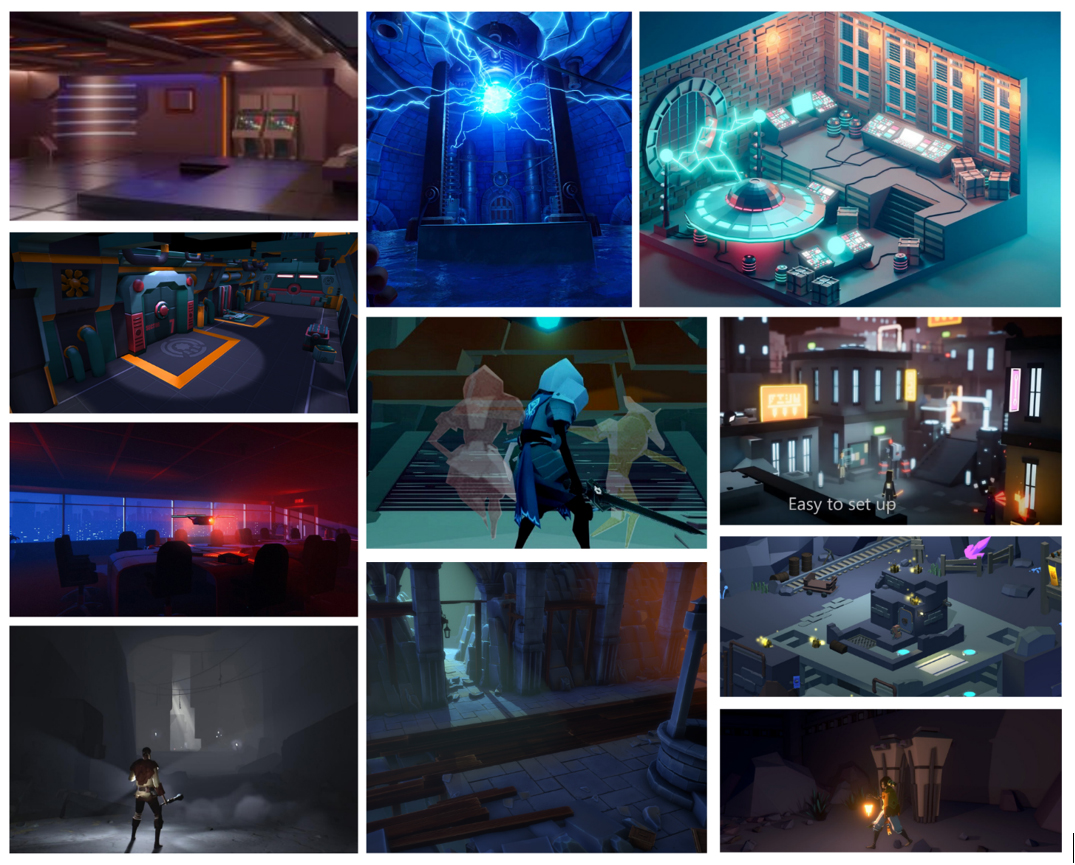
\includegraphics[width=0.8\linewidth]{content/pictures/Game_Atmo.jpg}
\caption{Moodboard des Spiel (Quelle: Moodboard, 2023)}
\label{fig:moodboard}
\end{figure}


\section{Art-Stil}
Wie bereits im Kapitel \nameref{sec:moodboard} angesprochen wurde, wird der Art-Stil des Spiels Low-Poly sein. Denkbar wäre es auch in \ac{HD} Texturen zu wechseln, um dadurch ebenfalls auf grafischer und Post-Processing Ebene mehr aus der Umwelt herauszuholen. Dazu im \nameref{sec:ausblick} mehr. Da das Spiel dem Steam-Punk Genre folgt, wird die Welt eher maschinell und viktorianisch aussehen.

\section{Aussehen des Chronologen}
Der Chronologe ist durch sein Aussehen und sein Verhalten ebenfalls in das Spielgenre und den Art-Stil integriert. Er wirkt wie ein vor sich hin tüftelnder Wissenschaftler, der eher wenig aus seinem Labor kommt. Er trägt eine Brille mit großen eckig-milchigen Brillengläsern. Dazu trägt er eine Weste mit einem Hemd darunter. Zu seiner Weste mit Hemd trägt er eine ledrige, festsitzende Hose. Außerdem trägt er in die Jahre gekommene Lederschuhe (vgl. Abbildung \ref{fig:chronologe}.

\begin{figure}[ht]
\centering
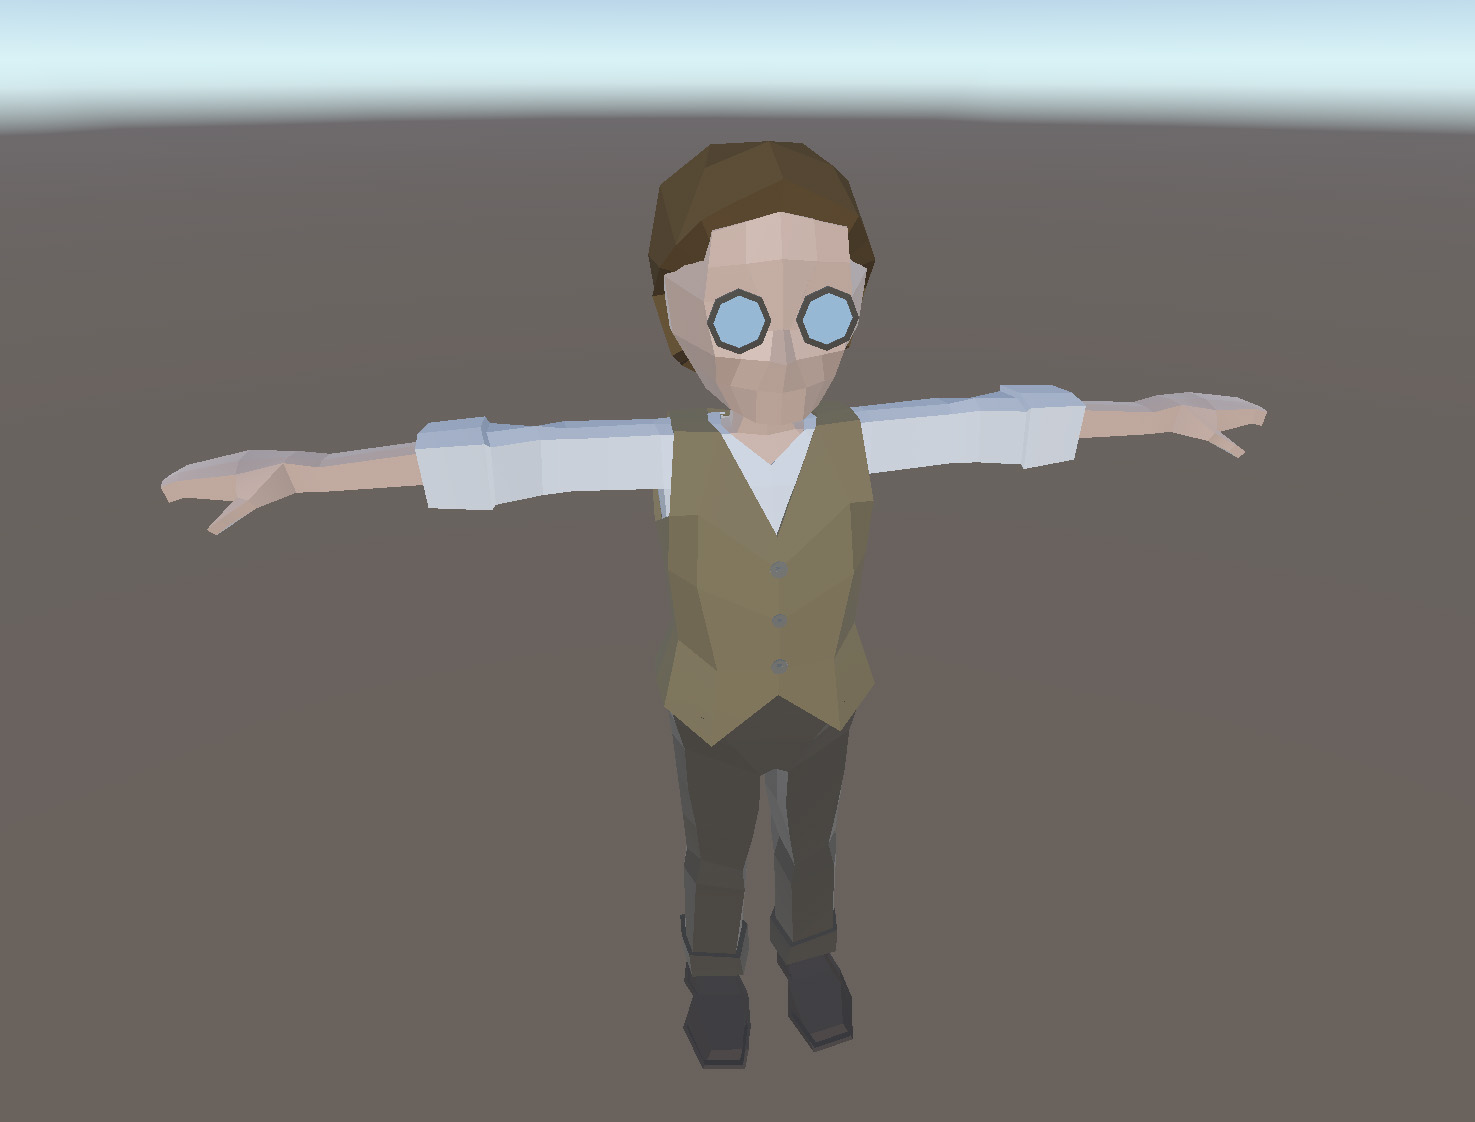
\includegraphics[width=0.8\linewidth]{content/pictures/Chronologe.jpg}
\caption{3D Modell Chronologe (Quelle: eigene Darstellung)}
\label{fig:chronologe}
\end{figure}

Im Kontext dieses Prototyps besitzen die Ich-Versionen des Chronologen unterschiedlich farbige Westen. Zum Beispiel hat der Chronologe aus den Zeitlinien des Tutorials eine blaue oder gelbe Weste. Diese Versionen des Chronologen kann man in Abbildung \ref{fig:chronologe_b} oder Abbildung \ref{fig:chronologe_y} sehen. Durch die farbliche Unterscheidung ist der Chronologe für den Spieler unterscheidbar. Beim Lösen der Rätsel ist es wichtig zu wissen, welches Ich des Chronologen gerade an den jeweiligen Elementen der Rätsel steht. Diese farbliche Unterscheidung wird im Laufe dieses Kapitel in Abschnitt \nameref{sec:user-interface} im Unterabschnitt \ref{sec:character-overview}.

\begin{figure}[ht]
\centering
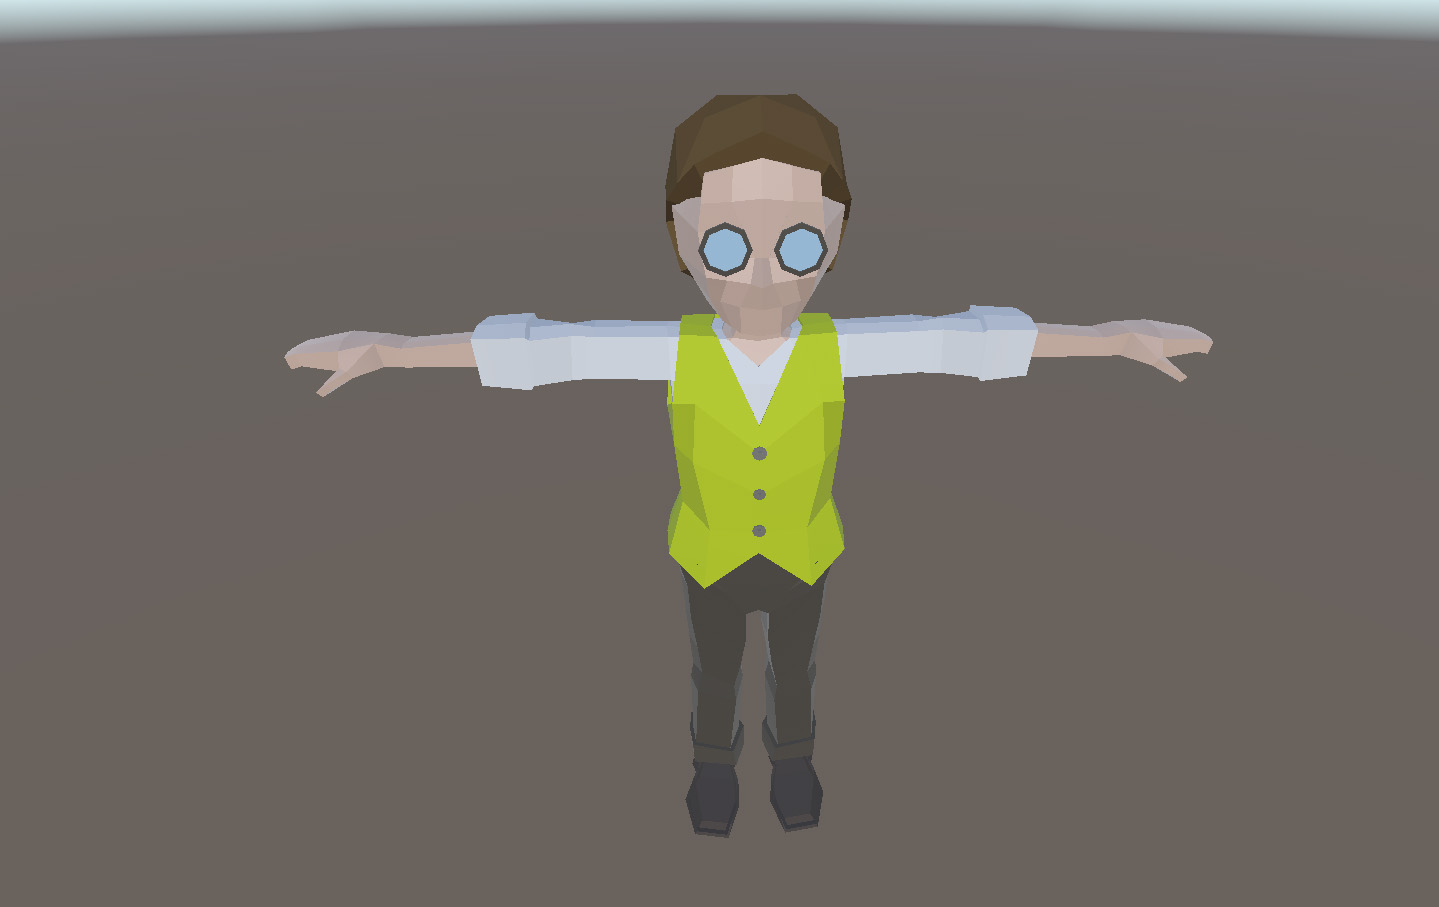
\includegraphics[width=0.8\linewidth]{content/pictures/Chronologe_y.jpg}
\caption{3D Modell Chronologe, gelbe Weste (Quelle: eigene Darstellung)}
\label{fig:chronologe_y}
\end{figure}

\begin{figure}[ht]
\centering
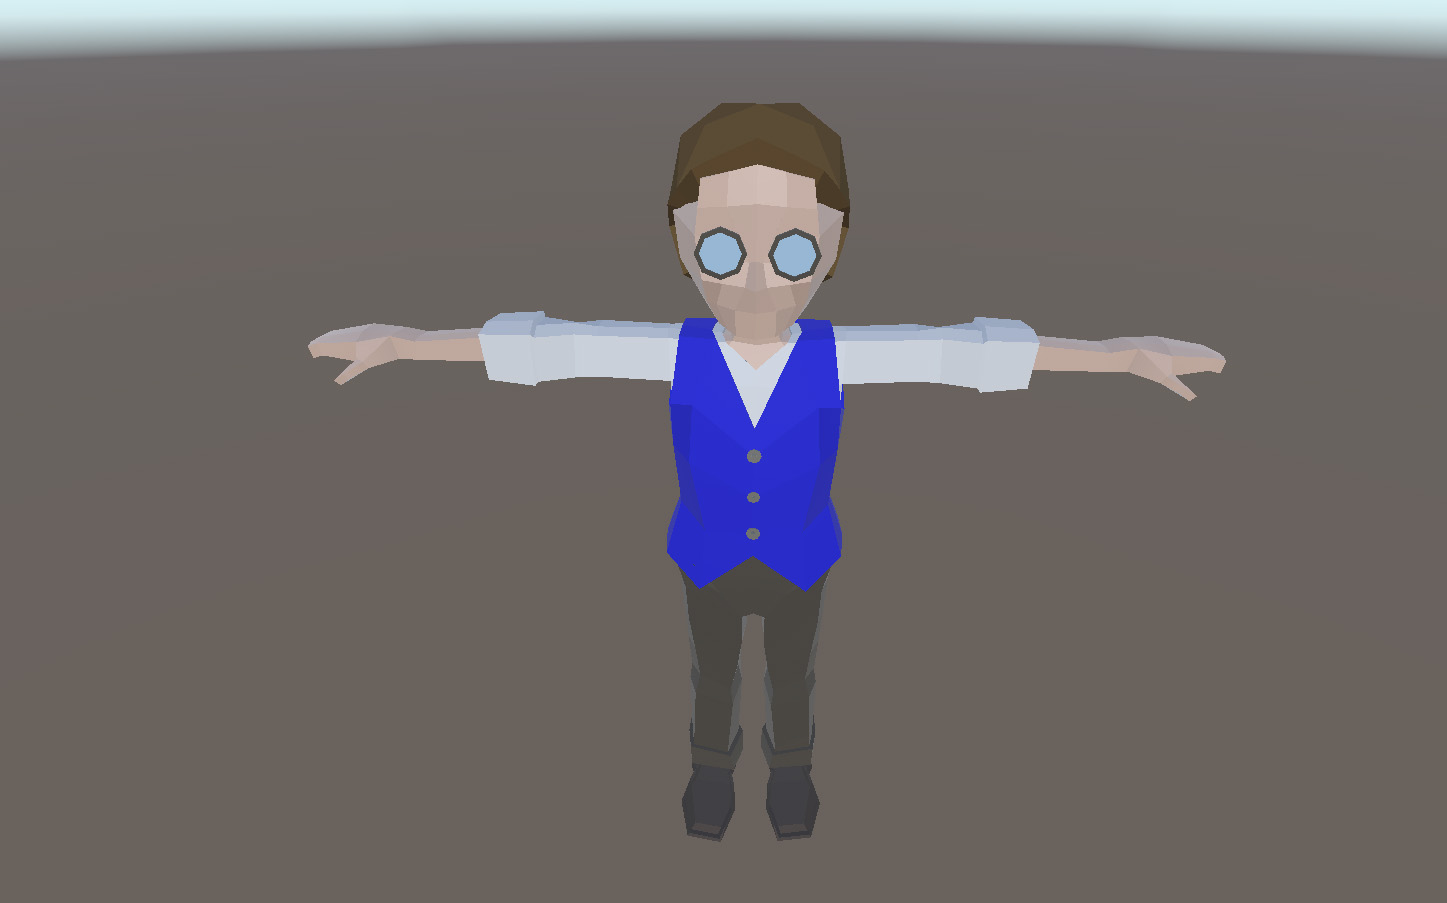
\includegraphics[width=0.8\linewidth]{content/pictures/Chronologe_b.jpg}
\caption{3D Modell Chronologe, blaue Weste (Quelle: eigene Darstellung)}
\label{fig:chronologe_b}
\end{figure}

Im Kontext der allgemeinen Konzeption besitzen die Chronologen, außer der Farbe, weitere Unterscheidungen, die aber nicht im Prototyp umgesetzt wurden. So tragen die Chronologen unterschiedliche Kleidungen und Accessoires. Zudem sind die Körper der Chronologen unterschiedlich entwickelt und besitzen dadurch auch eine unterschiedliche Größe. Es kann aber auch zu Arbeitsunfällen oder dergleichen gekommen sein, wodurch ein Arm oder Bein amputiert werden musste. Diese Unterschiede in der Geschichte der einzelnen Chronologen spiegelt sich auch auf das äußere des \ac{3D} Modells wieder. 

Der Spieler erhält dadurch für jede Zeitlinie ein unterscheidbares Aussehen des Chronologen. Dadurch kann er im Verlauf des Spiels die einzelnen Aufnahmen der jeweiligen Chronologen unterscheiden und zuordnen.

\subsection{Nicht mehr vom Spieler gesteuerte Chronologen}
Wie bereits in \nameref{sec:npc} beschrieben, wird der Platzhalter des Chronologen transparent in der Szene dargestellt. Wie in den Abbildungen \ref{fig:ghost_b} und \ref{fig:ghost} zu sehen, haben die \ac{3D}-Körper des Chronologen transparente Materialien. Dadurch wird der Eindruck erweckt, dieses Ich im Moment der Spielzeit noch nicht existiert und zeitlich gesehen in der Vergangenheit an dieser Stelle steht.

Das aufgenommene Ich des Chronologen, das in den Abbildungen \ref{fig:chronologe},\ref{fig:chronologe_y} und \ref{fig:chronologe_b}, wird als solches in der Szene dargestellt. Ein nicht transparentes Aussehen des Chronologen bewirkt hierbei den Eindruck, dass das Ich des Chronologen aus der entsprechenden Zeitlinie einen Einfluss auf die Spielwelt besitzt. Der Spieler kann sich nun anhand dieses Ichs orientieren und weiß, dass dieses Ich gerade in der Szene aktiv ist und nicht zu diesem Zeitpunkt nur in der Vergangenheit existiert.
\begin{figure}[ht]
\centering
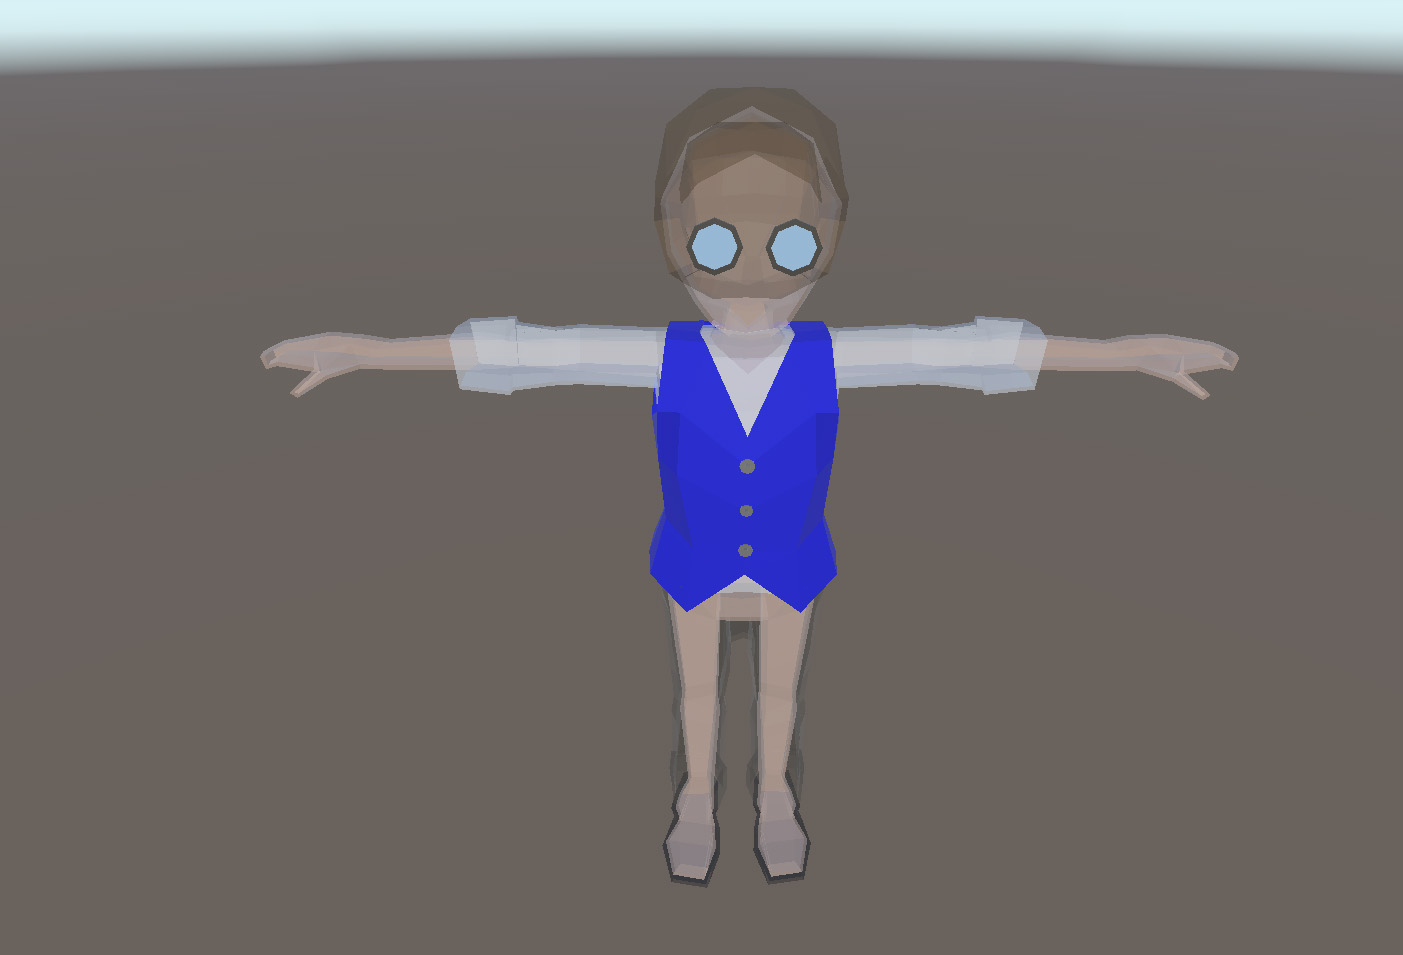
\includegraphics[width=0.8\linewidth]{content/pictures/Ghost_b.jpg}
\caption{3D Modell Geist, blaue Weste (Quelle: eigene Darstellung)}
\label{fig:ghost_b}
\end{figure}

\begin{figure}[ht]
\centering
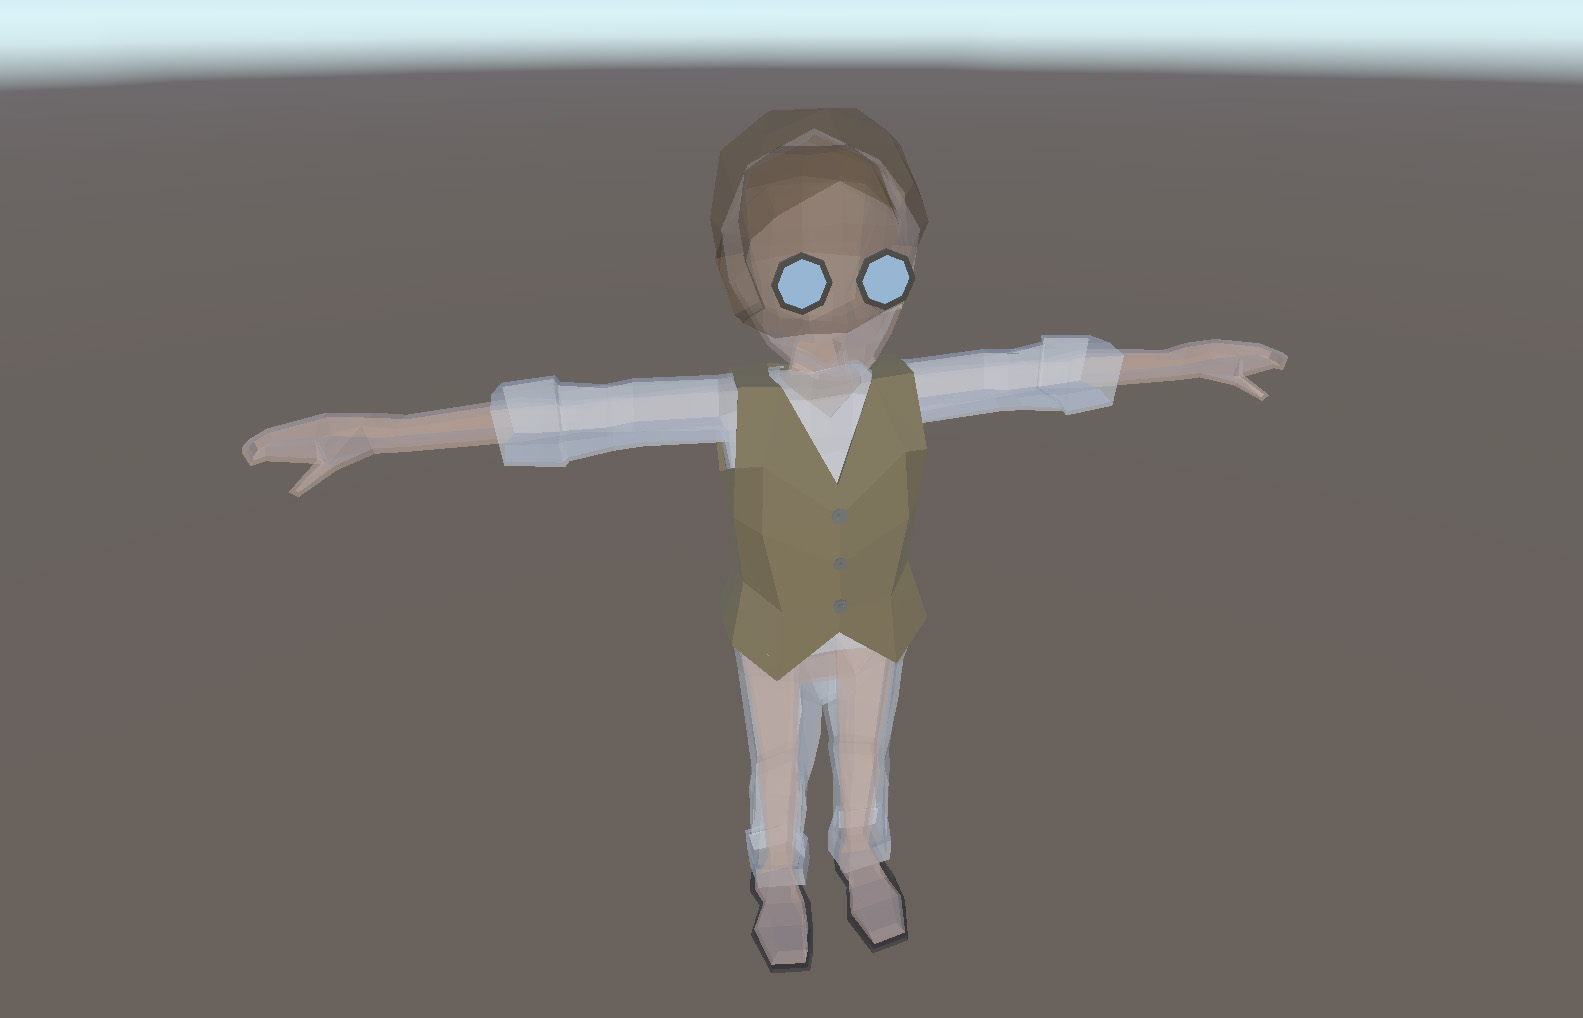
\includegraphics[width=0.8\linewidth]{content/pictures/Ghost.jpg}
\caption{3D Modell Geist (Quelle: eigene Darstellung)}
\label{fig:ghost}
\end{figure}

\section{User Interface}\label{sec:user-interface}
Im Folgenden werden die einzelnen Elemente der User-Interfaces vorgestellt und durch Mockups prototypisch visualisiert. Es handelt sich hierbei zum einen um das gesamte \ac{UI}, das der Spieler während des Spiels zu sehen bekommt und zum anderen um das \ac{UI} des Datenlesers, welches der Chronologe immer zur Hand hat.
\subsection{Graph}
\subsection{Timer}\label{sec:user_timer}
\subsection{Zeitkontinuum}\label{sec:kontinuum_ui}
\subsection{Charakter Übersicht}\label{sec:character-overview}
\subsection{Steuerhinweis}
\subsection{Dialoge}
\subsection{Systemfehler}
\subsection{Tragen von Objekten}
\subsection{Datenleser}\label{sec:datenleser_ui}
\section{Führung durch das Level}
Der Spieler erhält durch unterschiedliche Mechanismen eine Führung durch das Level. Dazu gehören unter anderem Partikelsysteme, Kletterkanten und Tooltips.
\subsection{Partikelsysteme}\label{sec:particle-system}
Dem Spieler soll an bestimmten Stellen wie an einer Druckplatte vermittelt werden, dass er auf diese stehen soll, um einen Mechanismus auszulösen.

\begin{figure}[ht]
\centering
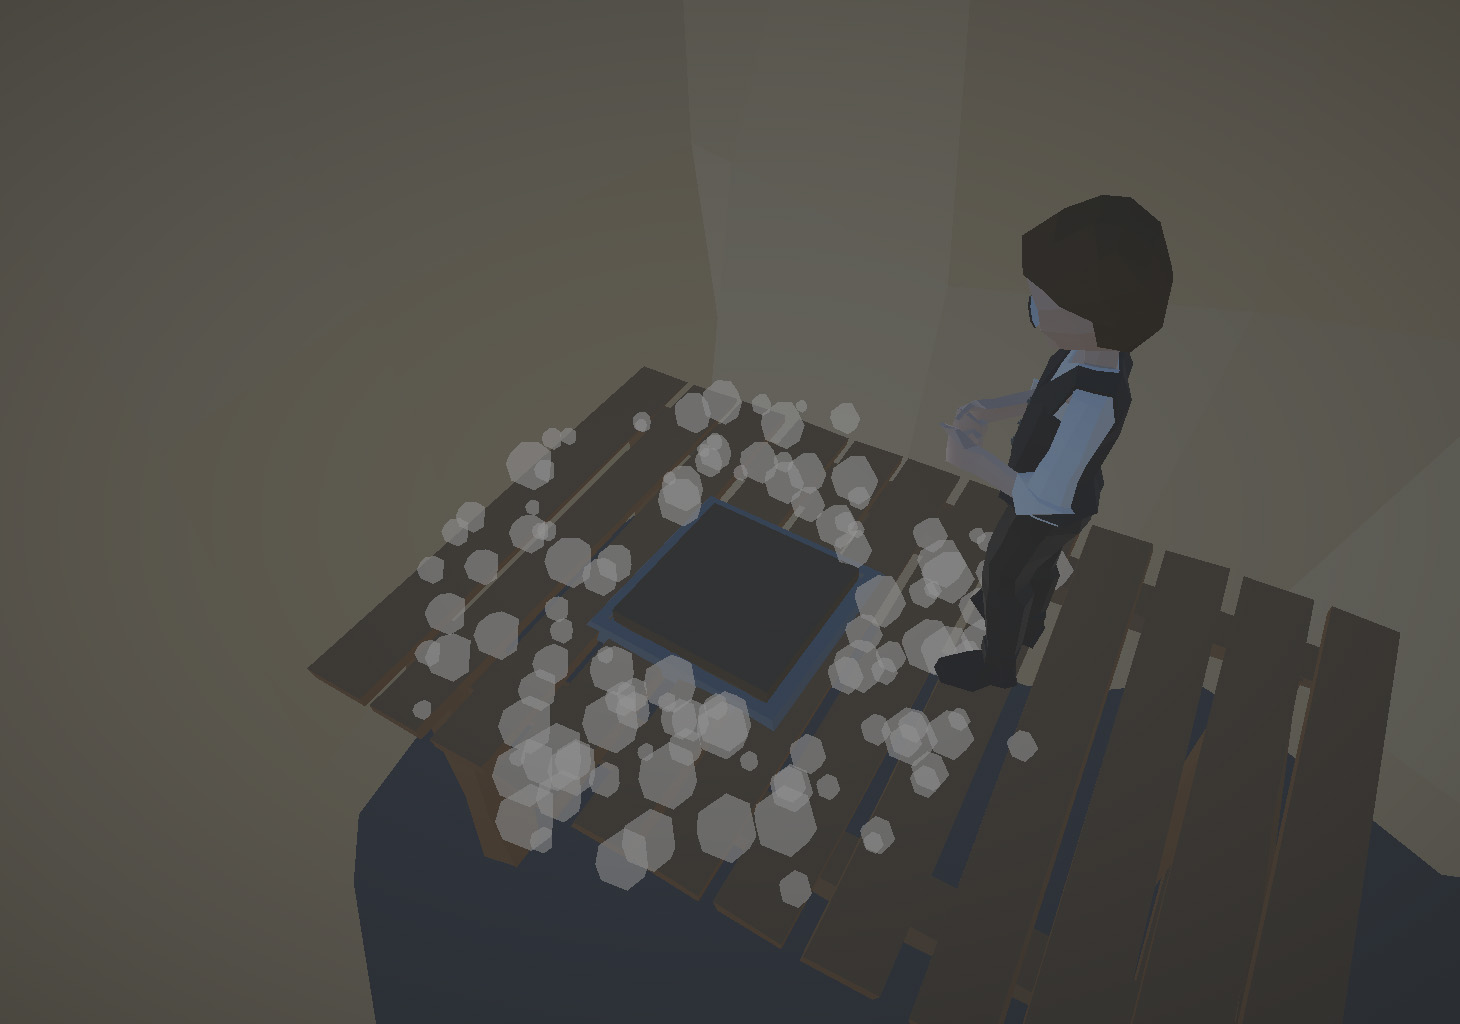
\includegraphics[width=0.8\linewidth]{content/pictures/Pressureplate_tooltip.jpg}
\caption{Partikelsystem Druckplatte, (Quelle: eigene Darstellung)}
\label{fig:pressureplate_tooltip}
\end{figure}

Wie in Abbildung \ref{fig:pressureplate_tooltip} zu sehen, wird, sobald der Chronologe nahe an einer Druckplatte steht, das Partikelsystem der Druckplatte aktiviert. Es zeigt durch seinen Fluss auf die Druckplatte dem Spieler an, dass er auf diese Druckplatte gehen muss, um sie durch seinen Körper zu aktivieren.

\subsection{Kletterkanten}\label{sec:leadge}
Ein Bestandteil der Bewegungsmöglichkeiten des Spielers ist es, auf Gerüste oder Stützen zu klettern. Hierbei benötigt der Spieler auf zwei Wege einen Hinweis darauf, wo und wie er auf Objekte klettern kann.
Der Spieler kann durch ein Kabel, das an der Kante des entsprechenden Objektes liegt, erkennen, dass er auf dieses klettern kann. Das Kabel wird durch eine Schraffierung an der Kante unterstützt.

\begin{figure}[ht]
\centering
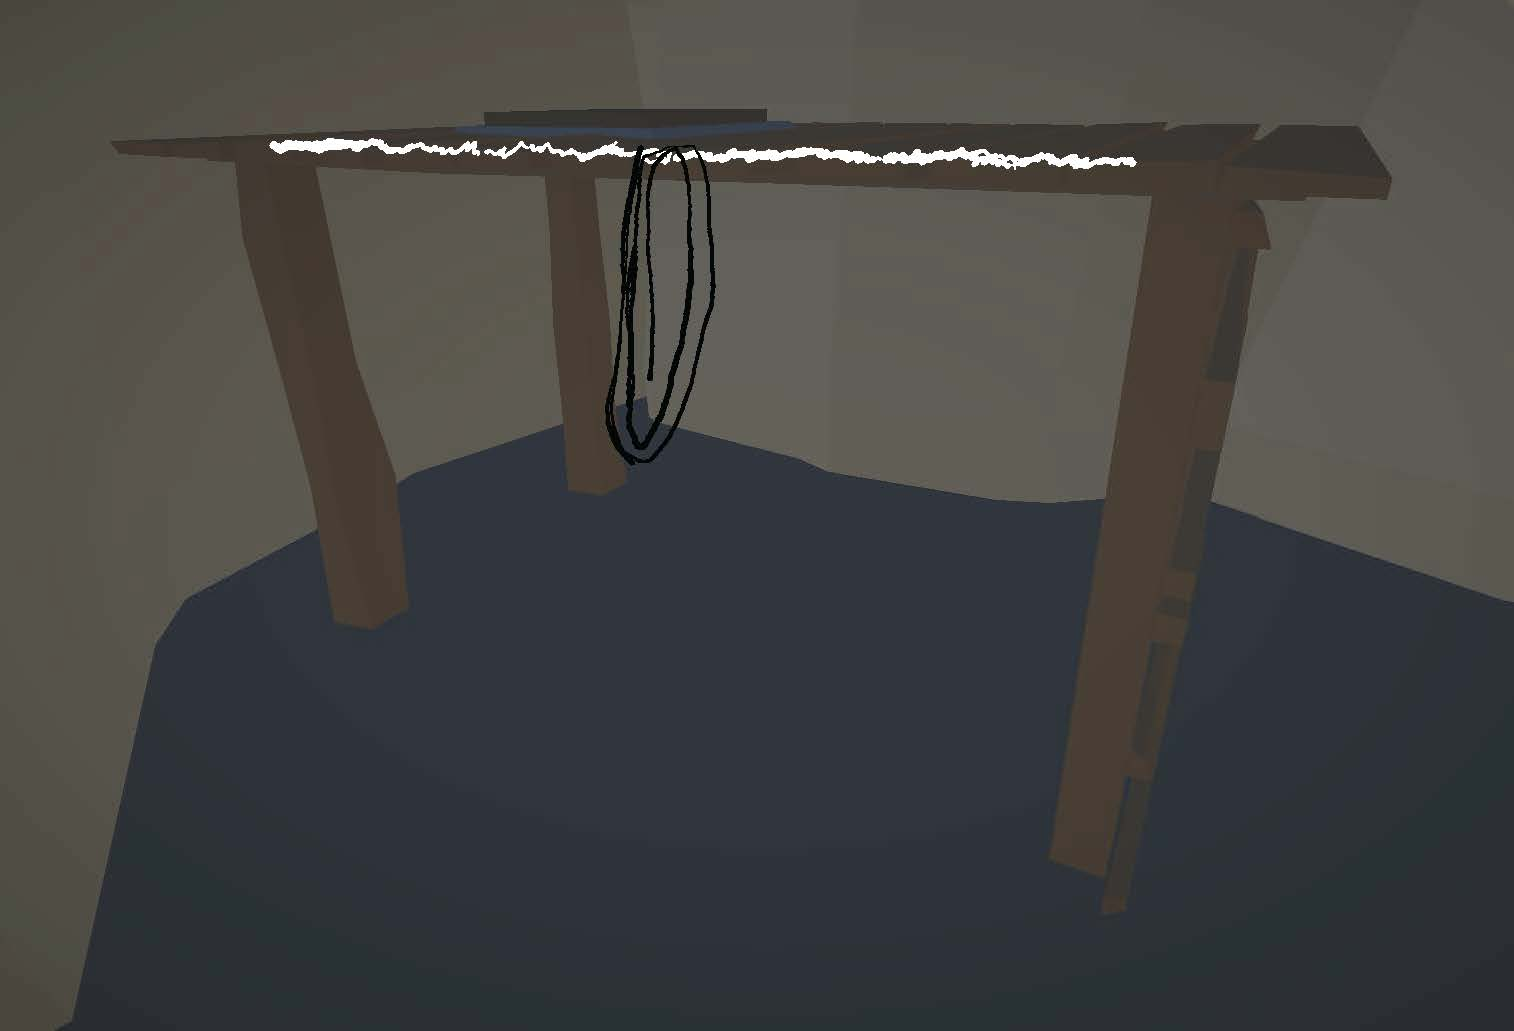
\includegraphics[width=0.8\linewidth]{content/pictures/leadge_wireframe.jpg}
\caption{Kantenmarkierung an Spielweltobjekten, (Quelle: eigene Darstellung)}
\label{fig:leadge}
\end{figure}

Wie in Abbildung \ref{fig:leadge} zu sehen ist, markiert die weiße Linie die Schraffierung der Kletterkante. Die Kante ist abgenutzt, weil bereits einige Menschen vor dem Chronologen auf dieses Gerüst geklettert sind. 
Die schwarze Markierung auf der Abbildung stellt ein Kabel dar, das von der Kante als Sicherung befestigt ist. Über dieses Kabel kann man sich hochziehen, ohne abzurutschen.

\subsection{Tooltips}\label{sec:tooltip}

In Bezug auf die Kletterkante aus Kapitel \ref{sec:leadge} erhält der Spieler eine zusätzliche visuelle Aufforderung, wie er mit der Kante zu interagieren hat. Diese Aufforderungen werden im Kontext dieser Arbeit Tooltips genannt. Diese Tooltips beinhalten einen Keycode der Tastatur, durch welchen der Spieler den Chronologen auf das Gerüst klettern lassen kann. Im Fall der Kletterkante ist es die Leertaste.

Weitere Gegenstände, mit denen der Chronologe interagieren kann, enthalten ein Tooltip. Zum Beispiel wird ein Tooltip angezeigt, sobald sich der Spieler einem Hebel nähert. Dies ist in Abbildung \ref{fig:lever_tooltip} oder in Abbildung \ref{fig:stair_tooltip} zu sehen. Bei der Treppe handelt es sich hierbei um ein tragbares Objekt. Der Spieler muss dieses Treppenbruchstück an einen anderen Ort platzieren.

\begin{figure}[ht]
\centering
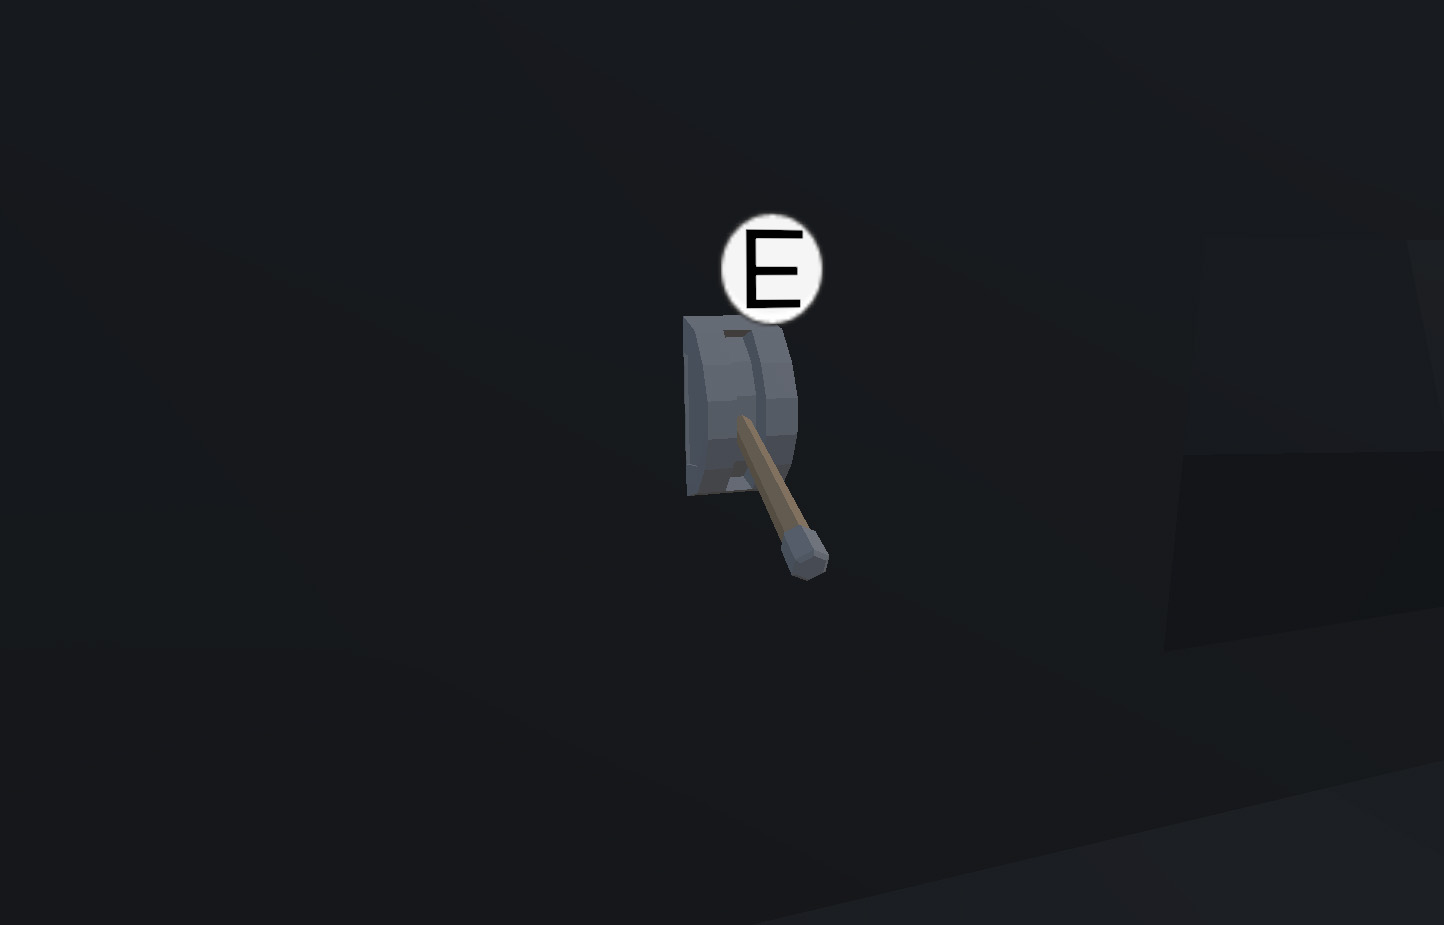
\includegraphics[width=0.8\linewidth]{content/pictures/lever_tooltip.jpg}
\caption{Hebel mit Tooltip, (Quelle: eigene Darstellung)}
\label{fig:lever_tooltip}
\end{figure}

\begin{figure}[ht]
\centering
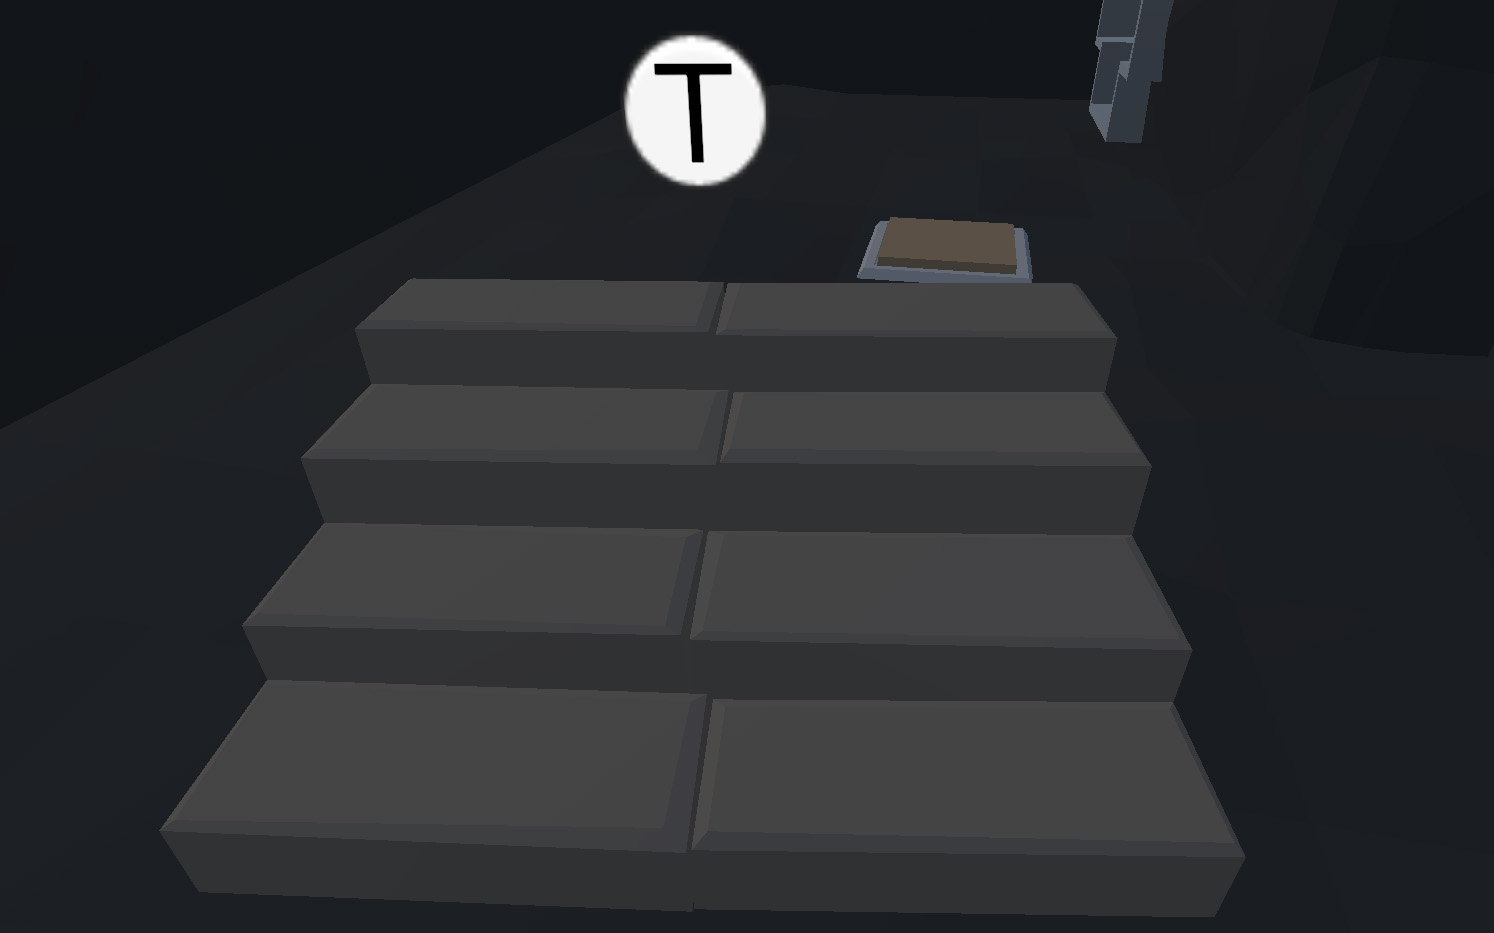
\includegraphics[width=0.8\linewidth]{content/pictures/carry_tooltip.jpg}
\caption{Treppe mit Tooltip, (Quelle: eigene Darstellung)}
\label{fig:stair_tooltip}
\end{figure}

Damit der Spieler ein besseres Verständnis dafür erhält, welche Interaktion er durch das Betätigen der Taste auslöst, wird der Name der Interaktion neben den Keycode positioniert. Diese Änderungen werden zu dem bislang implementierten Stand ergänzt und in den folgenden Abbildungen \ref{fig:stair_tooltip_title}, \ref{fig:lever_tooltip_title} und \ref{fig:leadge_title} dargestellt.

\begin{figure}[ht]
\centering
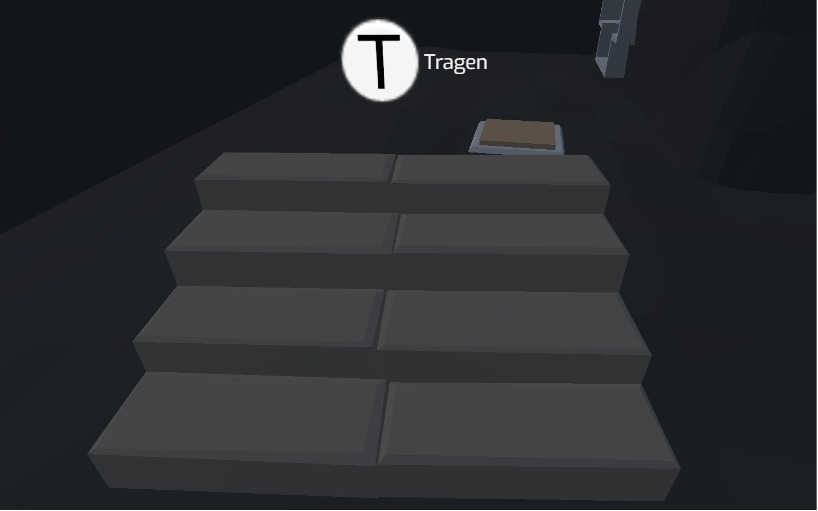
\includegraphics[width=0.8\linewidth]{content/pictures/stair_tooltip_title.jpg}
\caption{Treppe mit Tooltip und Aufforderung, (Quelle: eigene Darstellung)}
\label{fig:stair_tooltip_title}
\end{figure}

\begin{figure}[ht]
\centering
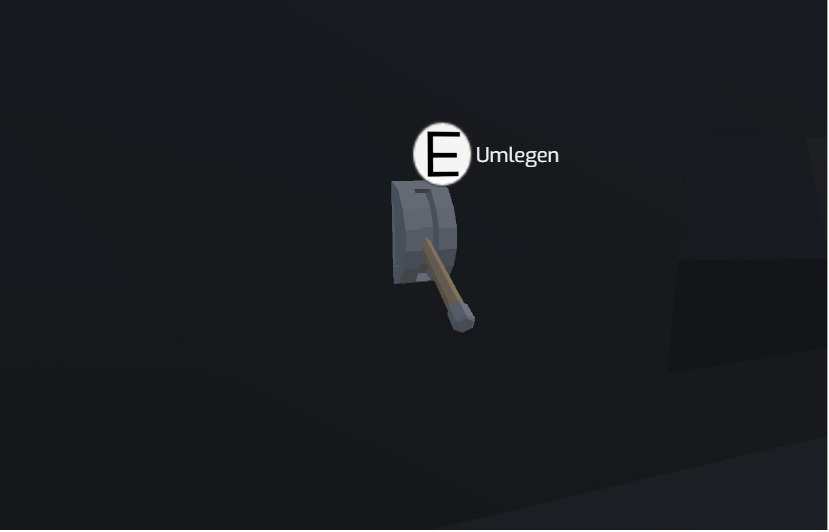
\includegraphics[width=0.8\linewidth]{content/pictures/lever_tooltip_title.jpg}
\caption{Hebel mit Tooltip und Aufforderung, (Quelle: eigene Darstellung)}
\label{fig:lever_tooltip_title}
\end{figure}

\begin{figure}[ht]
\centering
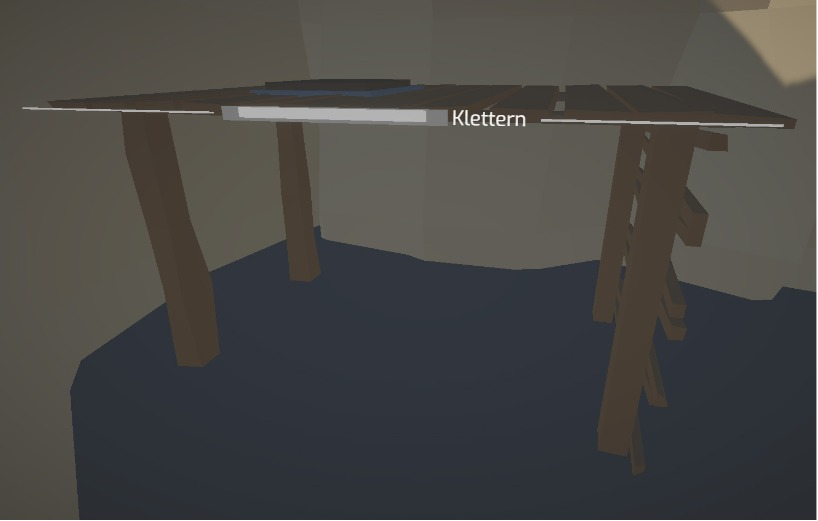
\includegraphics[width=0.8\linewidth]{content/pictures/leadge_tooltip_title.jpg}
\caption{Kante mit Tooltip und Aufforderung, (Quelle: eigene Darstellung)}
\label{fig:leadge_title}
\end{figure}

Dadurch versteht der Spieler schneller und besser, welche Interaktion er bewirkt. Er muss nicht zuerst im Datenleser nachlesen, welche Auswirkung seine Interaktion haben wird, sondern ist beim Betrachten des Tooltips bereits ersichtlich.

\section{Interaktionsgegenstände}
Im folgenden Kapitel werden verschiedene Objekte dargestellt, mit denen der Chronologe interagieren kann. In der Aufzählung werden zum einen die bislang bestehenden Objekte aufgezählt und zum anderen konzeptionelle Anpassungen, die die Objekte ergänzen, vorgestellt.
\subsection{Druckplatte}

\begin{figure}[ht]
\centering
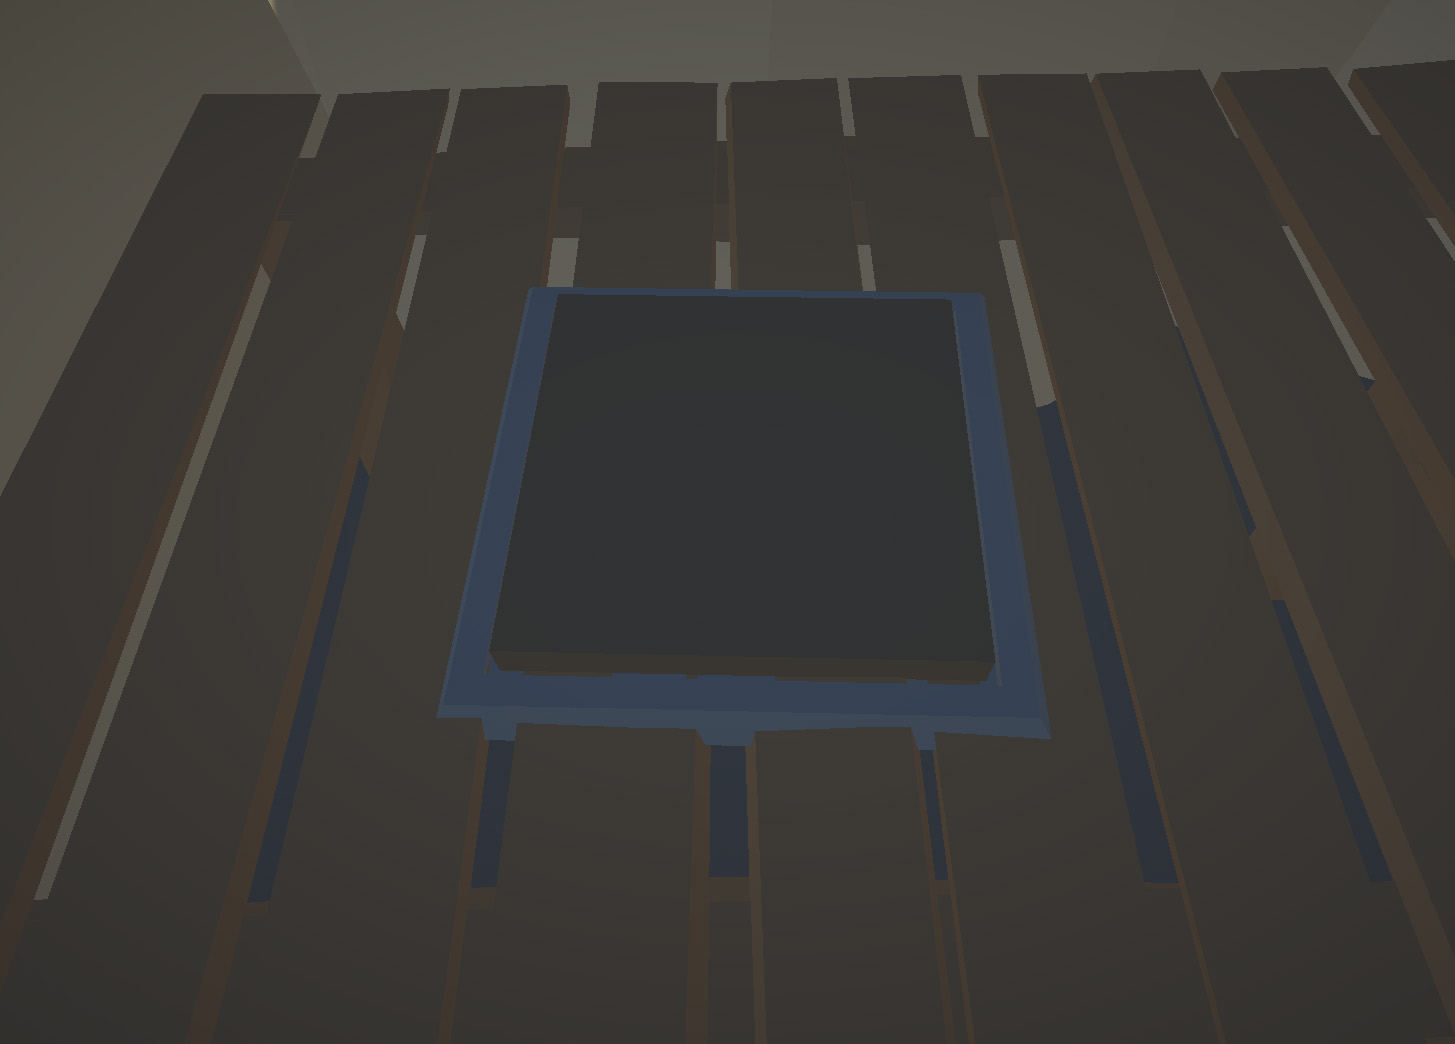
\includegraphics[width=0.8\linewidth]{content/pictures/Pressureplate.jpg}
\caption{Druckplatte, (Quelle: eigene Darstellung)}
\label{fig:pressureplate_interactable}
\end{figure}

Abbildung \ref{fig:pressureplate_interactable}: \nameref{fig:pressureplate_interactable} zeigt eine Druckplatte, wie sie in der Spielwelt eingebaut wurde. Der hölzerne Kern, stellt den Sensor dar, der eingedrückt wird, sobald das Gewicht des Chronologen auf ihm lastet. Jede Druckplatte enthält ein Partikelsystem, wie es in Abschnitt \ref{sec:particle-system} \nameref{sec:particle-system} bereits erklärt wurde.

\subsection{Hebel}

\begin{figure}[ht]
\centering
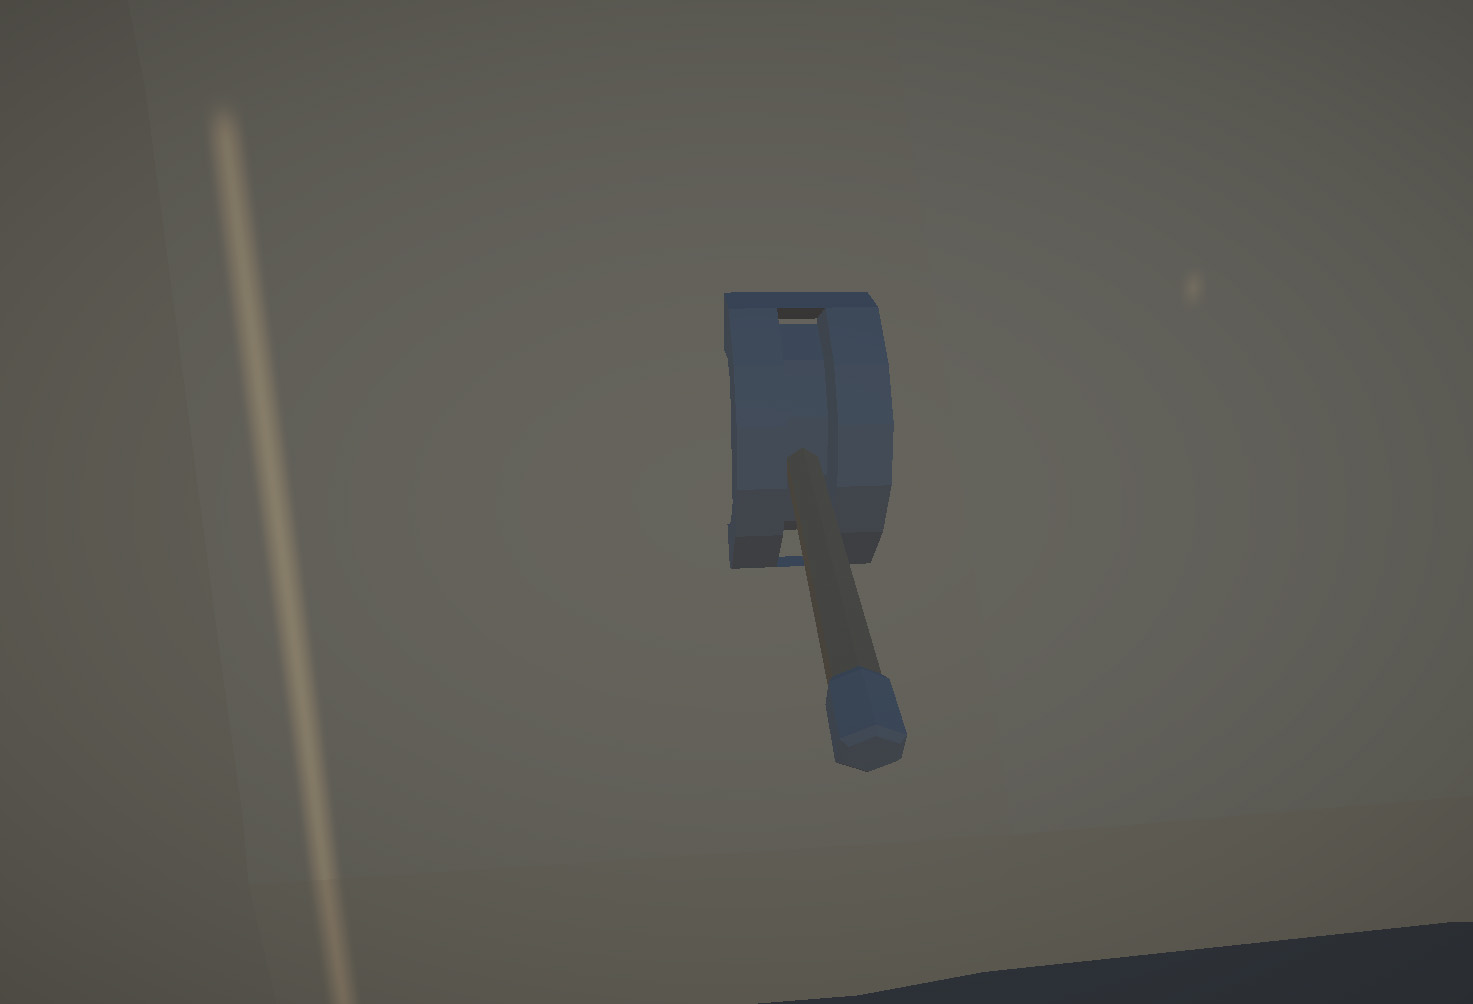
\includegraphics[width=0.8\linewidth]{content/pictures/Lever.jpg}
\caption{Hebel, (Quelle: eigene Darstellung)}
\label{fig:lever_interactable}
\end{figure}

Derzeit sind Hebel, wie sie in Abbildung \ref{fig:lever_interactable}: \nameref{fig:lever_interactable} zu sehen sind, in der Spielwelt verbaut. Sobald der Chronologe mit einem Hebel interagiert, fährt der Hebelstab nach oben und signalisiert dem Spieler, dass er aktiviert wurde. Abbildung \ref{fig:lever_interactable_active}: \nameref{fig:lever_interactable_active} zeigt einen aktivierten Hebel.

\begin{figure}[ht]
\centering
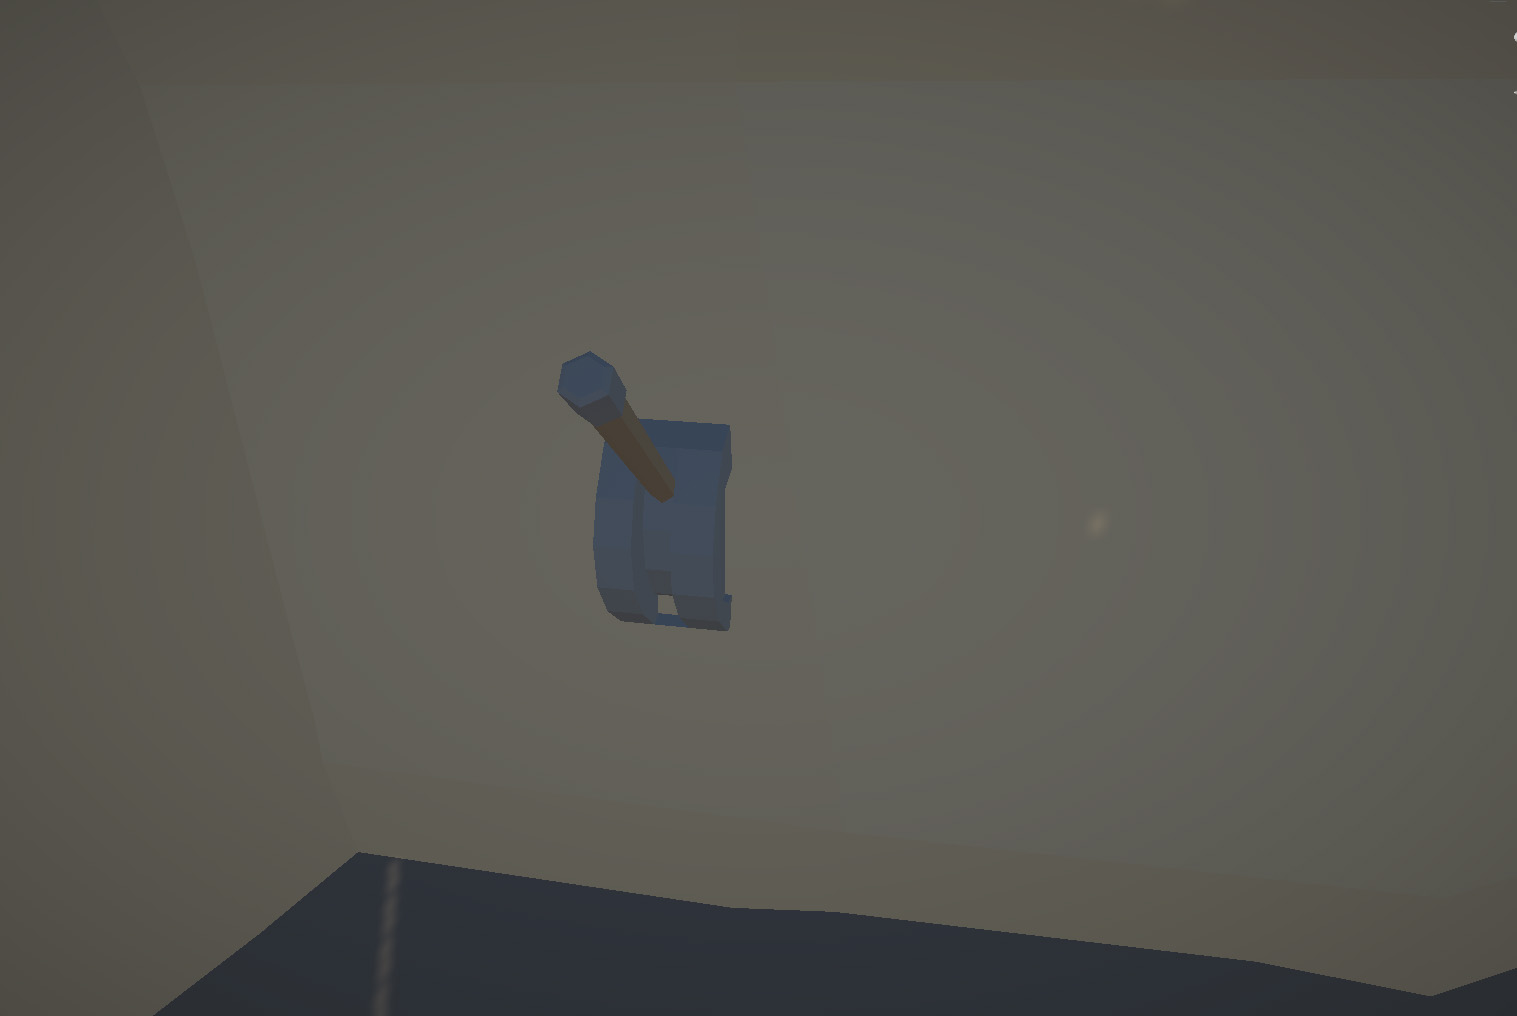
\includegraphics[width=0.8\linewidth]{content/pictures/Lever_active.jpg}
\caption{Mit Hebel wurde interagiert, (Quelle: eigene Darstellung)}
\label{fig:lever_interactable_active}
\end{figure}

Der Hebel bekommt ein separates Interface an die Seite gehängt, auf dem zwei Lampen zu sehen sind (vgl. Abbildung \ref{fig:lever_interactable_active_diods}: \nameref{fig:lever_interactable_active_diods}). Sobald die nur die obere grüne Lampe leuchtet, ist der Hebel aktiviert. Leuchtet nur die untere Lampe rot, so ist er deaktiviert. So erfährt der Spieler zusätzlich, wann ein Hebel aktiviert wurde und wann er deaktiviert ist.

\begin{figure}[ht]
\centering
\includegraphics[width=0.8\linewidth]{content/pictures/Lever_activator_diod.jpg}
\caption{Hebel mit Lampeninterface, (Quelle: eigene Darstellung)}
\label{fig:lever_interactable_active_diods}
\end{figure}

\subsection{Ventil}
Die Abbildungen \ref{fig:valve_01}: \nameref{fig:valve_01}, \ref{fig:valve_02}: \nameref{fig:valve_02} und \ref{fig:valve_03}: \nameref{fig:valve_03} zeigen drei unterschiedliche Versionen eines Ventils, mit denen der Spieler interagieren kann. 

\begin{figure}[ht]
\centering
\includegraphics[width=0.8\linewidth]{content/pictures/Vault.jpg}
\caption{Ventil Version 1, (Quelle: eigene Darstellung)}
\label{fig:valve_01}
\end{figure}

\begin{figure}[ht]
\centering
\includegraphics[width=0.8\linewidth]{content/pictures/Vault_02.jpg}
\caption{Ventil Version 2, (Quelle: eigene Darstellung)}
\label{fig:valve_02}
\end{figure}

\begin{figure}[ht]
\centering
\includegraphics[width=0.8\linewidth]{content/pictures/Vault_03.jpg}
\caption{Ventil Version 3, (Quelle: eigene Darstellung)}
\label{fig:valve_03}
\end{figure}

Wie bereits in Kapitel \ref{sec:ventil} \nameref{sec:ventil} angesprochen, muss der aktiv Zustand des Ventils nicht dauerhaft gehalten werden. Ein Ventil ist entweder dauerhaft aktiv oder inaktiv.

\subsection{Stützen}
Abbildung \ref{fig:stuetze_01}: \nameref{fig:stuetze_01} zeigt die Zeichnung einer Stütze, die der Spieler tragen muss und auf welcher er klettern kann. Diese dient als ein erster Entwurfsversuch für die im Level eingebaute Stütze, die in Abbildung \ref{fig:L02_R02_R02}: \nameref{fig:L02_R02_R02} durch einen gestreckten Würfel dargestellt wird. Jede Stütze hat Zahnräder an ihrer Oberfläche montiert, wodurch diese Stützen an laufende Zahnräder angeschlossen werden können, welche in späteren Leveln zu finden sein werden.
\begin{figure}[ht]
\centering
\includegraphics[width=0.2\linewidth]{content/pictures/Stuetze_01.jpg}
\caption{Zeichnung einer einfachen Stütze mit Zahnrädern, (Quelle: eigene Darstellung)}
\label{fig:stuetze_01}
\end{figure}

In Abbildung \ref{fig:stuetze_02}: \nameref{fig:stuetze_02} kann diese Anreihung besser betrachtet werden.  

\begin{figure}[ht]
\centering
\includegraphics[width=0.4\linewidth]{content/pictures/Stuetze_02.jpg}
\caption{Zeichnung einer Reihe an Stützen angeschlossen an Mechanismus, (Quelle: eigene Darstellung)}
\label{fig:stuetze_02}
\end{figure}

Die erste Stütze wird an den Beginn des Mechanismus´, ein aus der Wand ragendes Zahnrad, gestellt, sodass das Drehmoment des entsprechenden Zahnrades die Zahnräder an der Stütze drehen lässt. Anschließend muss eine zweite oder dritte Stütze an die erste Stütze gestellt werden, damit das Drehmoment weitergegeben werden kann. Diese Stützen werden verteilt in einem Raum zu finden sein. Die Aufgabe des Spielers ist es dann, diese in eine richtige Reihenfolge zu stellen.

\subsubsection{Treppe}
Die Stütze dient nicht als einziges tragbares Objekt in der Spielwelt, sondern es können auch verschiedenste Objekte sein. Als Beispiel für das in der Spielwelt integrierte tragbare Objekt dient eine Treppe, wie sie in Abbildung \ref{fig:stairs}: \nameref{fig:stairs} zu sehen ist.

\begin{figure}[ht]
\centering
\includegraphics[width=0.8\linewidth]{content/pictures/Stairs.jpg}
\caption{tragbares Treppenelement, (Quelle: eigene Darstellung)}
\label{fig:stairs}
\end{figure}

Dieses Treppenstück ist das Endstück einer Treppe, die der Spieler vervollständigen muss, um darüber auf bestimmte Objekte zu gelangen.

\subsection{Portal Steuereinheit}\label{sec:portal}
In der folgenden Abbildung \ref{fig:bsp_computer_03}: \nameref{fig:bsp_computer_03} ist ein erster Entwurf des Computers des Chronologen zu sehen. Das Interface, mit dem der Chronologe interagieren wird, besteht aus Kurbeln und vereinzelten Zahnrädern. Der Wissenschaftler kann über den kleinen Bildschirm seine Eingaben überprüfen und dem visuellen \ac{UI} des Computers folgen. Auf der Rückseite des Computers befinden sich weitere Zahnräder, die die Eingaben an die Dienste des Computers übermittelt. 

\begin{figure}[ht]
\centering
\includegraphics[width=0.6\linewidth]{content/pictures/bsp_computer_03.jpg}
\caption{Computer des Chronologen, erstes Konzept, (Quelle: Stable Diffusion)}
\label{fig:bsp_computer_03}
\end{figure}

Der Computer dient nicht nur der Aufnahme und Speicherung von Notizen, sondern auch dem Bedienen der Erfindung des Chronologen. Über diesen Computer kann der Spieler im Labor seine nächsten Ziele auswählen.

\begin{figure}[ht]
\centering
\includegraphics[width=0.6\linewidth]{content/pictures/portal_01.jpg}
\caption{Erster Entwurf Portal der Maschine, (Quelle: Stable Diffusion)}
\label{fig:portal_01}
\end{figure}

Über das Portal, das in Abbildung \ref{fig:portal_01}: \nameref{fig:portal_01} als ein erster Entwurf skizziert ist, kann der Spieler seine Entdeckungsreisen beginnen.

\subsection{Lore}

\begin{figure}[ht]
\centering
\includegraphics[width=0.6\linewidth]{content/pictures/Lore.jpg}
\caption{Lore, (Quelle: eigene Darstellung)}
\label{fig:lore}
\end{figure}

Wie in Abbildung \ref{fig:lore}: \nameref{fig:lore} abgebildet, kann der Spieler Loren in der Spielwelt verschieben. Es sind nicht nur Loren, die der Spieler verschieben kann, sondern alle Objekte mit einem entsprechendem Tooltip. Die Lore aus der oben genannten Abbildung, kann vom Spieler nach Abschließen des ersten Kapitels an das Gerüst schieben, dadurch hat er die Möglichkeit das Gerüst hinaufzuklettern.

\section{Gebrauchsgegenstände}
Im folgenden Kapitel werden visuelle Konzepte den Gebrauchsgegenständen vorgestellt. Es wird darauf eingegangen, welche Gegenstände bereits in ihrer Form umgesetzt wurden und welche nur auf konzeptioneller Ebene existieren.

\subsection{Steuereinheit}
Die Steuereinheit ist in zwei Teile zu unterteilen. Zum einen ist sie Teil der Maschine, die der Chronologe erfunden hat. Dabei besteht der stationäre Teil der Maschine aus den Abbildungen \ref{fig:bsp_computer_03}: \nameref{fig:bsp_computer_03} und \ref{fig:portal_01}: \nameref{fig:portal_01}. Der Chronologe hat das tragbare Gegenstück dazu immer bei sich.

\begin{figure}[ht]
\centering
\includegraphics[width=0.6\linewidth]{content/pictures/SplitDevice_markers.jpg}
\caption{Steuereinheit, (Quelle: eigene Darstellung)}
\label{fig:split_device_marker}
\end{figure}

Sobald der Spieler die Steuereinheit öffnet, sieht er das Gerät aus der Abbildung \ref{fig:split_device_marker}: \nameref{fig:split_device_marker}.

Diese Steuereinheit ist in fünf Abschnitte eingeteilt.

\subsubsection{1. Abschnitt, Zahnrad}
Jede Zacke des Zahnrades steht für das Ich aus den anderen Zeitlinien, die der Spieler zur Verfügung hat. Dabei wird jede Zacke des Zahnrades nach der Farbe des verfügbaren Ichs markiert. Die Farben dienen der Unterscheidbarkeit für den Spieler.
\subsubsection{2. Abschnitt, aktive Zacke}
Sobald der Spieler ein Ich des Chronologen über das Rad auswählt, so dreht er das Zahnrad entweder mit oder gegen den Uhrzeigersinn. Sobald eine Zacke des Zahnrades an die Position der Markierung 2 gedreht wird, wird der darin enthaltene Chronologe ausgewählt. 
\subsubsection{3. Abschnitt, Status des Chronologen}
Sobald über das Zahnrad ein Chronologe ausgewählt wurde, wird im Feld der Markierung 3, der Status des Chronologen, genauer gesagt seine einhergehende Zeitlinie im Zeitkontinuum angezeigt. Dabei geht der Betrachtungswinkel der Steuereinheit vom derzeitig gesteuerten Chronologen aus.
% \paragraph{Gesplittete Zeitlinie}:
\paragraph{Gesplittete Zeitlinie:}
Abbildung \ref{fig:split_status}: \nameref{fig:split_status} zeigt den Status einer gesplitteten Zeitlinie. Das bedeutet, der Spieler hat von seinem jetzigen Standpunkt in der Zeitlinien Hierarchie bereits einen \say{\emph{Split}} zu diesem Ich des Chronologen absolviert und ist auf seinen jetzigen anschließend \say{\emph{zurückgemergt}}. Zu diesem Chronologen kann der Spieler erst wieder wechseln, sobald die Zeitlinie dieses Chronologen nicht mehr aktiv ist.

\begin{figure}[ht]
\centering
\includegraphics[width=0.1\linewidth]{content/pictures/Splitet_icon_trnsp.jpg}
\caption{gesplitteter Zeitlinien Status, (Quelle: eigene Darstellung)}
\label{fig:split_status}
\end{figure}

\paragraph{Aktuelle Zeitlinie:}

Abbildung \ref{fig:current_status}: \nameref{fig:current_status} zeigt das Statussymbol der Zeitlinie, wenn eine Zacke an das Auswahlfeld gedreht wird, an dem der derzeitige Chronologe farblich markiert wurde.

\begin{figure}[ht]
\centering
\includegraphics[width=0.05\linewidth]{content/pictures/Current_icon_trnsp.jpg}
\caption{aktueller Zeitlinien Status, (Quelle: eigene Darstellung)}
\label{fig:current_status}
\end{figure}

\paragraph{Zeitlinie zum Zurückmergen:}

Sobald eine Zeitlinie den Status aus Abbildung \ref{fig:merge_status}: \nameref{fig:merge_status} besitzt, kann der Spieler auf dieses Ich des Chronologen \say{\emph{zurückmergen}}. 
Dabei springt er in der Zeit auf den letzten Zeitpunkt, die diese Zeitlinie erlebt hat, zurück. 
Nach der Auswahl dieses Ichs startet der \say{\emph{Mergvorgang}}.

\begin{figure}[ht]
\centering
\includegraphics[width=0.15\linewidth]{content/pictures/Merge_icon_trnsp.jpg}
\caption{Zeitlinienstatus zum Zurückmergen, (Quelle: eigene Darstellung)}
\label{fig:merge_status}
\end{figure}

\paragraph{Verfügbare Zeitlinie:}

Erscheint auf dem Feld keins der drei Symbole aus den Abbildungen \ref{fig:split_status}: \nameref{fig:split_status}, \ref{fig:current_status}: \nameref{fig:current_status} und \ref{fig:merge_status}: \nameref{fig:merge_status} so ist dieses Ich frei und kann für einen \say{\emph{Splitvorgang}} ausgewählt werden.

\subsubsection{4. Abschnitt, Name des Chronologen}

Auf dem oberen Anzeigeelement erscheint der Name des ausgewählten Chronologen. Zusätzlich zu der Position des Zahnrades kann der Spieler hierdurch feststellen, dass er das richtige Ich des Chronologen ausgewählt hat.

\subsubsection{5. Abschnitt, Auswahl bestätigen}

Über den Knopf auf dem Zahnrad kann der Spieler seine Auswahl bestätigen. Der Knopf verändert in Abhängigkeit der Auswahl seine Farbe. Die Farben weisen den Spieler darauf hin, ob er seine Auswahl bestätigen kann oder ob er gerade einen nicht verfügbaren Chronologen auswählen möchte. Der Knopf leuchtet grün, sobald die Auswahl auf einen freien Chronologen gefallen ist oder er auf einen Chronologen \say{\emph{zurückmergen}} möchte, oder rot, sobald er sein derzeitiges Ich oder ein \say{\emph{gesplittetes}} Ich ausgewählt hat.

\subsection{Datenleser}
Wie bereits in Kapitel \ref{sec:concept_datenleser} \nameref{sec:concept_datenleser} angesprochen, kann der Spieler über den Datenleser wichtige Informationen erhalten. 
Im derzeitigen Prototyp ist der Datenleser ein skalierter Würfel. Dieser dient lediglich als ein Platzhalter für das eigentliche \ac{3D}-Modell des Datenlesers.

\begin{figure}[ht]
\centering
\includegraphics[width=.5\linewidth]{content/pictures/Datenleser_vorderseite.jpg}
\caption{Vorderseite Datenleser, Konzeptzeichnung, (Quelle: Stable Diffusion)}
\label{fig:datenleser_front}
\end{figure}

\begin{figure}[ht]
\centering
\includegraphics[width=.5\linewidth]{content/pictures/Datenleser_rueckseite.jpg}
\caption{Rückseite Datenleser, Konzeptzeichnung, (Quelle: Stable Diffusion)}
\label{fig:datenleser_back}
\end{figure}

Die Abbildungen \ref{fig:datenleser_front}: \nameref{fig:datenleser_front} und \ref{fig:datenleser_back}: \nameref{fig:datenleser_back} zeigen einen ersten Konzeptentwurf, wie der spätere Datenleser aussehen kann.
Der Datenleser enthält ähnlich wie der Computer des Chronologen mechanische Elemente, über die die Eingaben erfolgen können. Diese Eingabeelemente wie Zahnräder und Kurbel befinden sich auf der Rückseite des Datenlesers. Über die Vorderseite erhält der Spieler nun das visuelle Interface, das bereits in Kapitel \ref{sec:datenleser_ui} \nameref{sec:datenleser_ui} vorgestellt wurde.

\subsection{Pager}

\begin{figure}[ht]
\centering
\includegraphics[width=.5\linewidth]{content/pictures/Pager_marks.jpg}
\caption{Pager, (Quelle: Stable Diffusion)}
\label{fig:pager}
\end{figure}

Die Abbildung \ref{fig:pager}: \nameref{fig:pager} zeigt ein erstes Konzept des Pagers, den der Spieler im späteren Verlauf des Spiels findet und erhält.

Über die mit der 1 markierten haptischen Interfaces aus Joystick ähnlichen Elementen und mechanischen Tasten kann der Chronologe die Eingabe des Spielers in das Gerät eingeben. Auf dem kleinen Bildschirm, der mit der 2 markiert ist, kann der Spieler seine Eingabe kontrollieren, ehe er sie mit einem Knopfdruck abschickt. Der Knopf ist das Element, das mit der 3 markiert wurde.

\subsection{Imitator}

\begin{figure}[ht]
\centering
\includegraphics[width=1\linewidth]{content/pictures/Imitator.jpg}
\caption{Imitator, (Quelle: eigene Darstellung)}
\label{fig:imitator}
\end{figure}

Wie in Abschnitt \ref{sec:concept_imitator} \nameref{sec:concept_imitator} angesprochen, erhält der Spieler nach Erreichen eines bestimmten Levels einen Imitator. Die Umsetzung des Imitators ist in Abbildung \ref{fig:imitator}: \nameref{fig:imitator} dargestellt.

Der Imitator ist in vier Abschnitte unterteilt.

\subsubsection{1. Abschnitt, Auswahlrad}
Über das Auswahlzahnrad kann der Chronologe die Zeit einstellen, wie lange die Kopie von ihm an der gesetzten Stelle stehen soll. Durch das Drehen des Zahnrades wird ein Mechanismus in der Sanduhr freigesetzt, die diese Zeit einstellt.

\subsubsection{2. Abschnitt, Bildschirm}
Über den Bildschirm, der auf der Oberseite des Imitators zu finden ist, kann der Spieler den über das Zahnrad gestellten Timer einsehen. Er hat die Wahlmöglichkeit zwischen 5, 10, 15, 30, 45, 60 und 90 Sekunden, die die Kopie des derzeitig aktiven Ichs des Chronologen an der derzeitigen Stelle imitiert. 

\subsubsection{3. Abschnitt, Auswahl bestätigen}
Über den Knopf in der Mitte des Zahnrades kann der Spieler seine Auswahl bestätigen.

\subsubsection{4. Abschnitt, Erstellung der Kopie}
Nachdem der Spieler seine Auswahl bestätigt hat, legt der Chronologe den Imitator an seine derzeitige Position. Dadurch wird die Kopie des derzeitigen Ichs in die Spielwelt gesetzt. Im Anschluss an den erfolgreichen Kopiervorgang hebt der Chronologe den Imitator wieder auf und verstaut ihn in seinen Taschen. Der Spieler erhält, wie in Abschnitt \ref{sec:user_timer} \nameref{sec:user_timer} gezeigt, unterhalb des Timers eine Ansicht, wie lange die Kopie noch aktiv ist.

\section{Menü}
Das Spiel besitzt zwei Arten von Menüs (Start und Pause). Das Startmenü erscheint immer nach dem Start der Anwendung, das Pausemenü kann in jedem Level des Spiels geöffnet werden. 

\subsection{Pause}

Der Spieler kann das Spiel über die \ac{ESC}-Taste pausieren. Dadurch öffnet sich der Datenleser des Chronologen und das Pausemenü erscheint auf dem Monitor des Datenlesers, worüber der Spieler Informationen über das Spiel nachlesen kann.

\begin{figure}[ht]
\centering
\includegraphics[width=1\linewidth]{content/pictures/StartScreen.jpg}
\caption{Pausemenü, (Quelle: eigene Darstellung)}
\label{fig:pausemenu}
\end{figure}

In der Abbildung \ref{fig:pausemenu}: \nameref{fig:pausemenu} ist ein Mockup des Pausemenüs zusehen, über das der Spieler das Spiel beenden, bestimmte Einstellungen ändern und das Spiel wieder fortsetzen kann.

\subsection{Start}

\begin{figure}[ht]
\centering
\includegraphics[width=1\linewidth]{content/pictures/StartScreen.jpg}
\caption{Startmenü, (Quelle: eigene Darstellung)}
\label{fig:mainmenu}
\end{figure}

Sobald das Spiel geladen hat, erscheint das in Abbildung \ref{fig:mainmenu}: \nameref{fig:mainmenu} zu sehende Startmenü des Spiels. Über dieses kann der Spieler seinen aktuellen Spielstand fortsetzen, ein neues Spiel starten, die Einstellungen öffnen oder das Spiel wieder verlassen.

\begin{figure}[ht]
\centering
\includegraphics[width=1\linewidth]{content/pictures/SoundSetting.jpg}
\caption{Toneinstellungen, (Quelle: eigene Darstellung)}
\label{fig:sound_settings}
\end{figure}

\begin{figure}[ht]
\centering
\includegraphics[width=1\linewidth]{content/pictures/CamSetting.jpg}
\caption{Kameraeinstellungen, (Quelle: eigene Darstellung)}
\label{fig:cam_settings}
\end{figure}

Im derzeitigen Prototyp kann der Spieler über das Einstellungsmenü in den Abbildungen \ref{fig:sound_settings}: \nameref{fig:sound_settings} und \ref{fig:cam_settings}: \nameref{fig:cam_settings} Ton- und Kameraeinstellungen tätigen. Über dieses Menü werden weitere Einstellungen getätigt werden können.

\section{Leveldesign}

Im Folgenden wird auf die umgesetzten Level des Prototyps eingegangen.

\subsection{Tutorial}

\begin{figure}[ht]
\centering
\includegraphics[width=1\linewidth]{content/pictures/Tutorial - A Fraction of Time.jpg}
\caption{Collage Tutorial, (Quelle: eigene Darstellung)}
\label{fig:collage_tutorial}
\end{figure}

Das erste Level im Prototypen ist das in Abbildung \ref{fig:collage_tutorial} \nameref{fig:collage_tutorial} gezeigte Tutorial. Es dient als Einführung in das Spiel. 

Das Setting des Tutorials ist ein verlassener Steinbruch, der nach dem Start der Maschine des Chronologen verlassen werden musste, weil die Arbeiter Angst vor einer Zeitlinienkonvergenz (vgl. Kapitel \ref{sec:konvergenz} \nameref{sec:konvergenz}) hatten. Der Spieler muss versuchen zu verstehen, wie er den Steinbruch für seine ehemaligen Bewohner wieder sicher gestalten und einen Schutz gegen eine Konvergenz aufbauen kann.
Dafür muss der Spieler das Level gründlich erforschen. In der Spielwelt sind Hinweise darauf versteckt, die der Spiele finden muss.

Nachdem der Spieler das erste Kapitel erfolgreich abschließen konnte, ist es ihm möglich in den Steinbruch erneut zurückzureisen, um ihn weiter zu erkunden. Dadurch hat er die Möglichkeit andere neue Elemente zu entdecken, wie  versteckte Gegenstände oder neue Wege zu finden das Level abzuschließen.

Diese Hinweise sind jedoch in dieser Version des Steinbruchs nicht integriert. Diese Spielwelt dient in diesem Prototyp als ein Tutorial, in dem der Hauptfokus auf dem Erlernen der Spielmechanik liegt. Im Vergleich zu einer fertigen Version des Spiels hat der Spieler in diesem Prototyp die Auswahl zwischen zwei weiteren Ichs des Chronologen. In einer fertigen Version wird der Spieler in seinem ersten Level nur mit einer weiteren Person des Chronologen starten. Dieser Steinbruch ist dabei ein zweites Level und nicht mehr das Tutorial. Diese Spielwelt wurde, deshalb als Tutorial ausgewählt, da sie zum einen dafür im Gamedesign Workshop konzipiert wurde und so die Spielmechanik verstanden werden konnte und zum anderen war sie bereits umgesetzt und konnte erneut verwendet werden. Ein neues Szenario für das Tutorial zu entwickeln war aus diesem Grund nicht sinnvoll, da der Fokus auch darauf bestand ein weiteres Szenario zu entwickeln, in dem neuartige Rätsel zu lösen sind.

\subsection{Labor}

\begin{figure}[ht]
\centering
\includegraphics[width=1\linewidth]{content/pictures/Labor - A Fraction of Time.jpg}
\caption{Collage Labor, (Quelle: eigene Darstellung)}
\label{fig:collage_labor}
\end{figure}

Dieser Prototyp umfasst ein zweites Level, welches Labor genannt wird. Dieses Level ist das letzte Level, um Kapitel 1 abzuschließen. Durch das Bestehen dieses Levels findet der Spieler einen Weg zurück in das Labor des Chronologen.

Wie in Abbildung \ref{fig:collage_labor} \nameref{fig:collage_labor} zu sehen ist, enthält das Laborlevel zusätzlich zu seinem Labor zwei verschiedene Räume. Der Spieler muss die Rätsel beider Räume lösen, um den Weg in das Labor zu öffnen. Sobald der Spieler in die Spielwelt eintaucht, macht er sich auf Anweisung des Ichs des Chronologen aus der Zeitlinie, in der sich das Labor befindet, auf den Weg zum Laboreingang. Im Eingangsraum zum Labor muss der Spieler und das Ich des Chronologen allerdings feststellen, dass die Eingangstür verschlossen ist und auch kein Strom angeschaltet wurde. Der Spieler muss nun in den Raum der zwei Kräne gehen, da er dort den Strom anstellen kann. Nachdem der Strom angestellt wurde, betritt der Spieler das Labor und findet einen Weg zurück in sein eigenes Labor.

Nach dem Betreten des Labors fällt dem Chronologen eine Ähnlichkeit zu seinem eigenen Labor auf. Es muss sich also um eine andere Version seines Labors handeln. Die Ähnlichkeit der Labore beruht darauf, dass durch die Zeitlinien Konvergenz am Anfang des Spiels Teile des Labors vom Chronologen in dieses Labor aus einer anderen Zeitlinie übergegangen sind. Darunter ist ein Teil der Maschine, durch welche der Chronologe in eine andere Zeitlinie reisen kann. Durch das gefundene Teil seiner Maschine kommt er in  sein eigentliches Labor zurück. Es befindet sich allerdings nicht mehr in der Zeitlinie des Chronologen, sondern an einem Ort ohne Raum und Zeit.

Der genaue Grund, wieso dieses Maschinenteil den Chronologen in sein Labor zurückführt, wird für den Spieler in der Handlung des fertigen Spiels behandelt. Sie wird in diesem Prototyp nicht erzählt.

Das Ich aus dieser Zeitlinie ist selbst kein Chronologe geworden. Allerdings forscht er ebenso wie der Chronologe in einem Labor in einer anderen Disziplin. Das Ich war in seiner Vergangenheit einmal in diesem Labor und wusste daher, wo sich der Eingang befinden würde und wo sich der Strom anstellen lässt.

Das gesamte Level besteht aus einem Höhlen- und Laborkomplex, welche mit einer alten Kanalisation verbunden sind. Durch die alten Röhren der Kanalisation kann der Spieler die einzelnen Räume der Spielwelt betreten.

Der Spieler hat für das Meistern des zweiten Levels zwei weitere Ichs zur Verfügung, da es sich im Vergleich zum Tutorial an einem späteren Zeitpunkt der Handlung befindet. 

\subsection{Labor des Chronologen}

\begin{figure}[ht]
\centering
\includegraphics[width=1\linewidth]{content/pictures/Collage Labor Chronologist.jpg}
\caption{Collage Labor des Chronologen, (Quelle: Stable Diffusion, UFO Laboratory by CG Plane)}
\label{fig:collage_labor_chron}
\end{figure}

Abbildung \ref{fig:collage_labor_chron} \nameref{fig:collage_labor_chron} gibt einen ersten Eindruck, wie das Labor des Chronologen aussehen wird. Zusätzlich zu dieser Collage besitzt das Labor, das aus \say{Kapitel \ref{sec:portal}: \nameref{sec:portal}} beschriebene Portal und seinen Computer. Über dieses Labor kann der Spieler wie bereits beschrieben seine zuvor erlebten Level erneut besuchen, ebenso seine kommenden Reisen starten.

Das Labor befindet sich an einem Ort ohne Raum und Zeit. Durch das erstmalige Benutzen der Zeitlinien-Reisemaschine erfolgte eine Zeitlinien Konvergenz, wodurch Teile des Labors in eine parallele Zeitlinie katapultiert wurden. Es entstehen Kopien des Labors, auf welche der Spieler am Ende des ersten Kapitels stößt. Das Labor als Ganzes blieb unbeschädigt, jedoch befindet es sich nicht mehr in der Zeitlinie des Chronologen.

\chapter{Umsetzung des Prototyps}\label{sec:dev}
Im Folgenden wird die Umsetzung des entwickelten Prototyps vorgestellt. Dabei werden zunächst die verwendeten Technologien vorgestellt. Anschließend erfolgt eine Analyse des alten Prototyps, auf deren Ergebnisse die Entwicklung einer neuen Version des Prototyps aufbaut. Im Anschluss wird das überarbeitete Replay und Aufnahmesystem des Prototyps vorgestellt. Zum Schluss wird das integrierte Soundsystem erklärt.

\section{Verwendete Technologien}
In der kommenden Aufzählung werden die verwendeten Unity Packages vorgestellt. Im Package Manager des auf der beiliegenden \ac{DVD} der Arbeit befinden sich mehr Packages im Registry, als hier aufgezählt werden. Das liegt daran, dass die hier genannten Pakete genutzt und die zusätzlichen Pakete im Registry zum Testen und für den Ausblick eingebunden wurden.

\subsection{Unity Version 2021.3.16f1}
Der Prototyp wurde in der Version 2021.3.16f1 \ac{LTS} umgesetzt. Diese Version war zum Startzeitpunkt der Thesis die aktuellste \ac{LTS} der 2021er-Version des Unity Editors. In ihr ist es für den Ausblick ebenfalls möglich, den Experimental-Release von \ac{DOTS} einzubinden. 
(vgl. \cite{noauthor_official_nodate})

\subsection{Blender 3.3.1}
Blender dient in der Umsetzung als Bearbeitungstool von \ac{3D} Objekten. Aufgrund der Tatsache, dass Blender (.blend) Dateien direkt in Unity integriert werden können, und nicht als \ac{FBX} exportiert und importiert werden müssen (vgl. \cite{technologies_unity_nodate}). Als die Umsetzung des Prototyps begann, war die Version 3.3.1 von Blender die aktuellste, die heruntergeladen wurde.

\subsection{Mixamo}
Die im Prototyp verwendeten Animationen des Spielercharakters stammen alle aus der Bibliothek von Mixamo. Mixamo ist in der Lage, importierte \ac{FBX} Modelle zu riggen. Dabei erhält das Objekt ein Skelett, welches animiert werden kann. Das dabei entstandene Skelett und die integrierten Animationen werden in diesem Prototyp verwendet.

\subsection{Envato Elements}
Über ein Abo bei Envato Elements konnten atmosphärische Sounds und Sounds und die der Spielercharakter im Spiel von sich gibt, heruntergeladen und eingesetzt werden.

\subsection{Cinemachine}
Die Cinemachine wird für die Kamerafahrt des Spiels verwendet. Durch sie ist es möglich, eine Third-Person-Sicht in das Spiel zu haben. Zusätzlich ist es möglich verschiedene virtuelle Kameras zu besitzen, durch welche zwischen Third- und First-Person Sicht des Spielers gewechselt werden kann. Durch sie ist es möglich, dass der Spieler den Chronologen in einer Third-Person Ansicht steuert und in einer First-Person-Ansicht seine Gebrauchsgegenstände sieht. Dadurch hat das Spiel eine immersive Wirkung.

\subsection{Filmbox Exporter}
Da der Prototyp dieser Arbeit auf einem Prototyp aus dem Gamedesign Workshop aufbaut, für den bereits einzelne \ac{3D} Modelle erstellt und eingebraut wurden, existieren schon einige \ac{3D} Modelle in der Bibliothek. Allerdings reichen diese nicht vollständig aus, um den Bedarf an \ac{3D} Objekten zu decken. Daher mussten Bibliotheken hinzugefügt werden. Diese werden in Kapitel \say{\ref{sec:extra-assets}: \nameref{sec:extra-assets}} aufgezählt. Diese \ac{3D}-Model Packages enthielten teilweise keine \ac{FBX} Dateien, weshalb über den \ac{FBX} Exporter diese aus Unity Prefabs erzeugt wurden. Das war insofern notwendig, da nicht alle \ac{3D} Modell dem Spielanspruch genügten und darüber hinaus nicht editierbar waren. Durch das Erstellen von \ac{FBX} Dateien aus den Prefabs, konnten diese in Blender importiert und bearbeitet werden. Um sie letztlich benutzen zu können, wurden diese wiederum im Unity Projekt abgespeichert und importiert.

\subsection{TextMeshPro}
TextMeshPro wird in der Kombination mit dem veralteten \say{Unity UI} und \say{legacy Text Mesh} als Darstellung und Text verwendet. Durch TextMeshPro werden alle \ac{UI} Elemente auf einer Canvas angezeigt. Das ermöglicht unter anderem, dass in einer späteren Version auch bspw. Videos im Datenleser eingebunden werden können.

\subsection{Universal Render Pipeline}
Im Unity Editor hat man die Möglichkeit eine Render Pipeline einzubinden oder nicht. In diesem Fall wurde entschieden, die \ac{URP} einzubinden. Dadurch besteht die Möglichkeit der Kamera ein Post-Processing einzubinden, wodurch spezielle Effekte und das Rendering der Spielwelt verändert werden kann. Im Abschnitt \ref{sec:paradoxon-stability} \nameref{sec:paradoxon-stability} wurden Effekte erwähnt, die auf das visuelle der Spielwelt wirken werden. Diese Effekte werden zukünftig über die \ac{URP} eingebunden und visualisiert.

\subsection{Unity Prefab Assets}\label{sec:extra-assets}
Zum Start der Entwicklung dieses Prototyps gab es bereits einige erstellte \ac{3D} Modelle, die in die Szenen eingebaut wurden. Die im Gamedesign Workshop erstellen \ac{3D} Modell haben allerdings nicht ausgereicht und so wurden aus anderen Packages \ac{3D} Modell importiert:

% \subsubsection{Fissure: Low Poly Caverns}
% Das zweite Level des Prototyps spielt wie bereits erwähnt in einem Labor- und Höhlensystem. Für das Höhlensystem wurden Assets aus diesem Package verwendet.

% \subsubsection{Low Poly Rock Models}
% Um die Höhle weitere auszugestalten, wurden über dieses kostenlose Asset Package weitere Stein Modelle eingebunden.

% \subsubsection{Low Poly Underground Mega Pack}
% Das Höhlensystem im zweiten Level wurde zum Teil aus den Modellen des \say{Low Poly Underground Mega Packs} gebaut. Sie inkludieren weitere Tunnelsysteme, welche für weitere Rätsel- und Level-Elemente genutzt werden kann. 

% \subsubsection{Steampunk Low Poly Pack}
% Das Genre des Spiels liegt im Steampunk. Für dieses Setting wurden weitere \ac{3D}-Assets benötigt, um das vorhandene Level auszuschmücken und das zweite Level aus ihnen zu bauen.

% \subsubsection{Victorian Low Poly Pack}
% Selbiges gilt für das \say{Victorian Pack}, das, wie es der Name sagt, auch in ein Steampunk Setting passt. Steampunk spielt zur Zeit der Viktorianischen Zeit und ergänzt das oben benannte \say{Steampunk Pack}.
\begin{itemize}  
    \item Fissure: Low Poly Caverns \cite{noauthor_fissure_nodate}
    \item Low Poly Rock Models \cite{noauthor_low_lprm}
    \item Low Poly Underground Mega Pack \cite{noauthor_low_nodate}
    \item Steampunk Low Poly Pack \cite{noauthor_steampunk_lp}
    \item Victorian Low Poly Pack \cite{noauthor_victorian_nodate}
    \item Unity Particle Pack \cite{noauthor_unity_nodate}
\end{itemize}


\section{Ausgangssituation}
Wie in Kapitel \say{\ref{sec:intro}: \nameref{sec:intro}} beschrieben, existiert ein erster kleiner Prototyp des Spiels aus dem Gamedesign Workshop. Dieser ist jedoch sehr anfällig für Fehler und noch unstrukturiert. Das liegt zum einen daran, dass vier verschiedene Personen mit einem unterschiedlichen Wissensstand in Unity an diesem Prototyp gearbeitet haben. Zum anderen liegt es daran, dass im grundlegenden Aufbau der Mechanik von einem falschen Ausgangspunkt ausgegangen wurde. Zu Beginn der Entwicklung wurde das Erstellen von verschiedenen Version des Chronologen als Ausgangspunkt angesehen, welcher zu Problemen führte. Zusätzlich war ein Teil des damaligen Konzepts eine Ursache dafür, dass das Bauen des Graphenbaums zu Fehlern führte. Dabei war die Idee, dass der Spieler eine bereits erstellte Zeitlinie erneut \say{\emph{Splitten}} kann, um sie zu ändern. In dem überarbeiteten Konzept ist diese Möglichkeit nun verschwunden. Im Folgenden werden auf die Aspekte eingegangen, die von ihrer Grundidee wichtig für die Umsetzung sind. Ebenso werden die  Aspekte beschrieben, die es zu überarbeiten gilt.
\subsection{Übernommene Aspekte}
\subsubsection{Aufbau eines Baumes aus Zeitlinien}\label{sec:good_01}
Der Spieler erstellt durch die Auswahl eines Ichs des Chronologen eine Zeitlinie, auf welcher sich dieses Ich zeitlich bewegen wird. Dazu wird zunächst eine Hauptwurzel des Baumes benötigt, welcher im folgenden Codeausschnitt zu sehen ist:
\begin{lstlisting}[caption={Ausschnitt aus GraphController aus dem alten Prototypen}, label={sec:old_graphController}]
public class GraphController : Controller
{
    [SerializeField]
    private Timeline rootTimeline;
    [SerializeField]
    private Timeline currentTimeline;
    [SerializeField]
    private List<Timeline> timelinesToHandle = new List<Timeline>();
...
}
\end{lstlisting}
\label{sec:rootTimeline_pld}

\begin{figure}[ht]
\centering
\includegraphics[width=1\linewidth]{content/pictures/Schaubild Timeline.jpg}
\caption{Schaubild zu Codeausschnitt „Ausschnitt aus Timeline aus dem alten Prototyp“, (Quelle: eigene Darstellung)}
\label{fig:codesnippet_timeline}
\end{figure}

Sowohl diese Hauptzeitlinie als auch die angegliederten Zeitlinien besitzen eine Liste an angegliederten Zeitlinien und eine Referenz an die Zeitlinie, an welche sie angegliedert wurden. Zudem erhalten diese Zeitlinien ein Level, auf welcher Ebene der Verschachtelung sie sich befinden (vgl.: folgender Codeausschnitt \ref{sec:old_timeline}).

\begin{lstlisting}[caption={Ausschnitt aus Timeline aus dem alten Prototyp}, label={sec:old_timeline}]
public class Timeline
{
    [SerializeField]
    private int _level = 0;
    [SerializeField]
    private List<Timeline> _children = new List<Timeline>();
    [SerializeField]
    private float _startTimestamp;
    [SerializeField]
    private CharacterData _player;
    [SerializeField]
    private Timeline _parent = null;
    [SerializeField]
    private Shadow _ghost = null;
    [SerializeField]
    private string ID;
    [SerializeField]
    private float[] _startPosition = new float[3];
    private SavePlayerData _data = null;
    ...
    public void InsertChild(Timeline child)
    {
        if(!children.Contains(child))
        {
            _children.Add(child);
        }
        else
        {
            _children.Insert(children.FindIndex(a => a.GetId() == child.GetId()),child);
        }
    }
    ...
}
\end{lstlisting}

In Abbildung \ref{fig:L02_E02_04_L01} \nameref{fig:L02_E02_04_L01} wird ein solcher Baum aufgezeigt. Die schwarze Zeitlinie ist dabei die $rootTimeline$ aus \ref{sec:rootTimeline_pld} \nameref{sec:rootTimeline_pld}. Diese Zeitlinie besitzt das Level 0. Umso weiter die Zeitlinien ineinander verschachtelt werden, steigt das Level der Zeitlinien. Sobald der Spieler nun das erste Mal \say{\emph{splittet}}, wird diese neue Zeitlinie (aus der Abbildung die blaue Zeitlinie) über die Methode $InsertChild()$ an die $\_rootTimeline$ angegliedert. Zusätzlich erhält dieses Child auch eine Referenz auf seinen Parent. Jedes angegliederte Child besitzt das Level des Parents plus 1: $\_level = \_parent.level +1$. Das Level der blauen Zeitlinie beträgt nun 1. Erzeugt der Spieler viele parallele  Zeitlinien, so wie die rote Zeitlinie aus der Abbildung \ref{fig:L02_E02_04_L01} \nameref{fig:L02_E02_04_L01}, so haben diese ebenfalls das Level 1. Hierbei wird nicht unterschieden, die wievielte Zeitlinie in den Children diese ist. 

\subsubsection{Welche Zeitlinien müssen nach einem Mergevorgang betrachtet werden?}\label{sec:good_02}
Nach einem \say{\emph{Mergevorgang}} wird die aktuelle Zeitlinie durch eine bereits existierende Zeitlinie ersetzt. Befindet sich der Spieler in Abbildung \ref{fig:merge-definition} auf der blauen Zeitlinie, so wechselt er zum Beispiel auf die schwarze Zeitlinie zurück. Ist dieser Wechsel abgeschlossen, so müssen die nach einem Split entstandenen rote und blaue Zeitlinie betrachtet werden.

\begin{lstlisting}[caption={HandleMerge Methode aus dem alten Prototyp}, label={sec:old_merge}]
public class GraphController
{
...
    private void HandleMerge(Player player)
    {
        float startPoint = -1;
        Timeline timeline = GetTimelineOfNewPlayer(player.GetCharacterData());
        if (timeline != null)
        {
            List<Timeline> childrenOfNewTimeline = timeline.GetChildren();
            if (childrenOfNewTimeline.Count > 1)
            {
                foreach (Timeline child in childrenOfNewTimeline)
                {
                    if (child.GetId().Equals(currentTimeline.GetId()))
                    {
                        startPoint = child.GetStartTimestamp();
                    }
                }
            }
            if (childrenOfNewTimeline.Count == 1)
            {
                foreach (Timeline child in childrenOfNewTimeline)
                {
                    startPoint = child.GetStartTimestamp();
                }
            }
            if (startPoint != -1)
            {
                TimeController.Instance.SetGameTime(startPoint);
                _currentTimeline = timeline;
            }
            HandleRemoveOldCharacter(_rootTimeline);
            timelinesToHandle = new List<Timeline>();
            CheckForInteractions(_rootTimeline);
        }
    }
    ...
}
\end{lstlisting}


Durch das \say{\emph{Splitting}} werden neue Verzweigungen in der $rootTimeline$ hinzugefügt, welche nun durch eine rekursive Methode durchforstet werden können. Folgende Methode wird wie im vorherigen Codeausschnitt \ref{sec:old_merge} am Ende der $HandleMerge()$ Methode aufgerufen. Es wird überprüft, welche Zeitlinien in dem Baum das gleiche oder ein höheres Level haben als die derzeitig aktive Zeitlinie. Durch die Überprüfung $!timeline.GetId().Equals(\_currentTimeline.GetId())$ wird ausgeschlossen, dass es sich hierbei um die aktuelle Zeitlinie handelt.

\begin{lstlisting}[caption={HandleMerge Methode aus dem alten Prototyp}, label={sec:old_checkForInteractions}]
public class GraphController
{
...
    private void CheckForInteractions(Timeline timeline)
    {
        if (timeline.GetLevel() >= _currentTimeline.GetLevel())
        {
            if (!timeline.GetId().Equals(_currentTimeline.GetId()))
            {
                timeline.ResetData();
                timelinesToHandle.Add(timeline);
            }
        }

        List<Timeline> children = timeline.GetChildren();
        if (children.Count > 0)
        {
            foreach (Timeline child in children)
            {
                CheckForInteractions(child);
            }
        }
    }
    ...
}
\end{lstlisting}

Trifft der Fall zu, dass $timeline.GetLevel() >= \_currentTimeline.GetLevel()$ dem Wert \say{true} entspricht, so werden diese Zeitlinien in eine Liste abgespeichert, welche die zu beachtenden Zeitlinien enthält.

\subsubsection{Wann sind die zu beachtenden Zeitlinien aktiv?}\label{sec:good_03}
\begin{lstlisting}[caption={Haupt Gameloop der Mechanik aus dem Gamedesign Workshop}, label={sec:handleGameTime_old}]
public class GraphController
{
...
    public void HandleGameTime(float gametime)
    {
        PurgeOldTimelines(gametime);
        if (_timelinesToHandle != null && _timelinesToHandle.Count > 0)
        {
            foreach (Timeline timeline in _timelinesToHandle.ToArray())
            {
                Shadow ghost = timeline.GetGhost();
                if (ghost != null)
                {
                    ghost.ReconstructRecord(gametime);
                }
                else
                {
                    if (timeline.IsTimestampStillValid(gametime))
                    {
                        if (timeline.GetStartTimestamp() <= gametime)
                        {
                            Shadow shadow = _playerController.CreateShadow(timeline.GetPlayer());
                            Vector3 positionVector = new Vector3(timeline.GetPosition()[0], timeline.GetPosition()[1], timeline.GetPosition()[2]);
                            shadow.gameObject.transform.position = positionVector;
                            timeline.InsertGhost(shadow);
                            shadow.ReconstructRecord(gametime);
                        }
                    }
                }
                if (!timeline.IsTimestampStillValid(gametime))
                {
                    _timelinesToHandle.Remove(timeline);
                }
            }
        }
    }

    private void PurgeOldTimelines(float gametime)
    {
        if (_currentTimeline.GetId().Equals(rootTimeline.GetId()))
        {
            HandlePurge(gametime, _rootTimeline);
        }
    }
    private void HandlePurge(float gametime, Timeline timeline)
    {
        List<Timeline> children = timeline.GetChildren();
        if (children.Count > 0)
        {
            foreach (Timeline child in children.ToArray())
            {
                HandlePurge(gametime, child);
            }
        }
        else
        {
            if (!timeline.IsTimestampStillValid(gametime))
            {
                timeline.GetParent()?.GetChildren()?.Remove(timeline);
            }
        }
    }
    ...
}
\end{lstlisting}

Der $TimeController$ des Prototyps übergibt an den $GameController$ über die Methode $HandleGameTime()$ den aktuellen Zeitpunkt des Timers. Sofern ein \say{\emph{Mergvorgang}} absolviert wurde, existiert auch eine Liste an zu beachtenden Zeitlinien. Diese $\_timelinesToHandle$ werden nun seriell durchgegangen. Dabei wird zunächst geprüft, ob diese Zeitlinie eine Kopie des Chronologen besitzt, der die Aufnahme der Zeitlinie reproduziert. Falls bislang noch keine Kopie existiert, wird geschaut, ob die übergebene $\_gametime$ bereits größer ist als die letzte in der Zeitlinie aufgenommene Interaktion. Trifft das zu, wird die Zeitlinie aus der Liste, der $\_timelineToHandle$ entfernt. Trifft es nicht zu und ist der übergebene Zeitpunkt größer oder gleich des Startpunktes der Zeitlinie, so wird eine Kopie erstellt und der Zeitpunkt wird an diese Kopie übergeben.

Im letzten Schritt wird in der Methode $HandlePurge()$ überprüft, welche erstellten Zeitlinien gelöscht werden können, da ihre letzte aufgenommene Interaktion im Vergleich zur $\_gametime$ in der Vergangenheit erfolgte und sie deshalb nicht mehr beachtet werden muss. Diese Methode wird allerdings nur dann aufgerufen, sofern der Spieler den Hauptchronologen steuert und sich auf der $_rootTimeline$ befindet.

\subsubsection{Wie rekonstruiert die Kopie des Chronologen die aufgenommene Interaktion?}\label{sec:good_04}
\begin{lstlisting}[caption={Rekonstruktionsmethode aus der Shadow.cs}, label={sec:reconstructing_old}]
public class Shadow : Player
{ 
...
    public void ReconstructRecord(float timestamp)
    {
        if(_interactions.Count > 0)
        {
            _lastInteraction  = _interactions.OrderByDescending(item => item.TimeStamp).First();
        }
        InteractionSaveData interaction = _interactions.Find(i => (float.Equals(i.TimeStamp,timestamp)));
        SetLastTimestamp(timestamp);
        if(interaction != null)
        {
            InteractionType type = (InteractionType)Enum.Parse(typeof(InteractionType),interaction.Type);
            switch(type)
            {
                case InteractionType.WALK:
                    MoveShadow(interaction.Target);
                    break;

                case InteractionType.JUMPSTART:
                    MoveShadow(interaction.Source);
                    gameObject.GetComponent<AnimationHandler>().jump();
                    break;

                case InteractionType.JUMPSTOP:
                    MoveShadow(interaction.Source);
                    gameObject.GetComponent<AnimationHandler>().stopJump();
                    break;

                default:
                    break;
            }
        }
        if(_lastInteraction != null && _lastInteraction.TimeStamp < timestamp)
        {
            Destroy(this.gameObject);
            DestroyShadow?.Invoke();
        }
    }
    private void MoveShadow(GameObjectSaveData data)
    {
        Vector3 positionVector = new Vector3(data.Position[0], data.Position[1], data.Position[2]);
        Vector3 moveVector = new Vector3(positionVector.x - transform.position.x, 0, positionVector.z - transform.position.z);
        transform.forward = moveVector;
        transform.position = positionVector;
        transform.localScale = new Vector3(data.Scale[0], data.Scale[1], data.Scale[2]);
        gameObject.GetComponent<AnimationHandler>().SetGhostPosition(positionVector);
    }
    ...
}
\end{lstlisting}

Der GraphController übergibt in der $HandleGameTime$ Methode den derzeitigen Zeitpunkt des Timers über die Methode $ shadow.ReconstructRecord();$ an die $Shadow$ Klasse weiter. In der dieser Methode wird aus der Liste der aufgenommenen Interaktionen die Interaktion gesucht, die zu diesem übergebenen Zeitpunkt passiert ist. Die durch diesen Aufruf gefundene Interaktion: $\_interactions.Find(i => \\(float.Equals(i.TimeStamp,timestamp)))$ wird nun in im \say{Switch-Case} ausgewertet. Bei diesem Prototyp konnte der Spieler nur laufen und springen.
Der Mechanismus der Rekonstruktion erfolgt nur in der $SHadow$ Klasse.

\subsubsection{Wie wurden die Interaktionen aufgenommen?}\label{sec:good_05}

\begin{lstlisting}[caption={Aufnahme von Bewegungen, Ausschnitt aus MovementAbility.cs}, label={sec:movementAbility_old}]
public class MovementAbility : Ability
{
    ...
    protected override void HandleInput()
    {
        float horizontal = Input.GetAxisRaw("Horizontal");
        float vertical = Input.GetAxisRaw("Vertical");
        Vector3 direction = new Vector3(horizontal, 0f, vertical).normalized;
        if (direction.magnitude >= 0.1)
        {
         //code was taken from the following video: https://www.youtube.com/watch?v=4HpC--2iowE line 12-14, 17-18
            float targetAngle = Mathf.Atan2(direction.x, direction.z) * Mathf.Rad2Deg + _cam.eulerAngles.y;
            float angle = Mathf.SmoothDampAngle(_playerTransform.eulerAngles.y, targetAngle, ref _turnSmoothVelocity, _turnSmoothTime);
            Vector3 moveDir = Quaternion.Euler(0f, targetAngle, 0f) * Vector3.forward;
            if (!GetComponent<Animator>().GetBool("isJump"))
            {
                _playerTransform.rotation = Quaternion.Euler(0f, angle, 0f);
                _controller.Move(moveDir.normalized * _speed * Time.deltaTime);
                if (!_cam.parent.GetChild(2).GetChild(3).GetComponent<AudioSource>().enabled)
                {
                    AudioPlayerScript.instance.playSpecificAudio("walking");
                }
            }
            if (GetComponent<Animator>().GetBool("isJump"))
            {
                _controller.Move(GetComponent<JumpAbility>().GetJumpdirection() * _speed / 3 * Time.deltaTime);
            }
            SubmitAction(InteractionType.WALK, this.gameObject.GetComponent<Player>(), this.gameObject, this.gameObject.transform, TimeController.Instance.GetGameTime());
        }
        else
        {
            if (_cam.parent.GetChild(2).GetChild(3).GetComponent<AudioSource>().enabled)
            {
                AudioPlayerScript.instance.stopSpecificAudio("walking");
            }
        }
        if (GetComponent<Animator>().GetBool("isJump"))
        {
            _controller.Move(GetComponent<JumpAbility>().GetJumpdirection() * _speed / 3 * Time.deltaTime);
        }
    }
    ...
}
\end{lstlisting}

Wie bereits in den Grundlagen erwähnt, muss das Aufnehmen und Abspielen der Interaktionen in einem deterministischen System stattfinden. Unity ist grundlegend nicht deterministisch. Deswegen werden beim Abspeichern der Bewegungen des Spielercharakters alle Zustände in den gerenderten Frames abgespeichert. Dieses Vorgehen hat Jonathan Blow beim Rewind-System in the Braid verwendet (vgl. \cite{gdc_implementation_2016}). Sein Vorgehen besagt, dass Positionen oder in diesem Fall Interaktionen nicht interpoliert werden, sondern in einem 1:1 Abbild abgespeichert werden sollen. Dadurch wird ein fehlerhaftes Reproduzieren vermieden. Daher war die Überlegung, die Bewegungs-Interaktion des Spielercharakters in jedem seiner bewegten Frames in Form einer Interaktionsklasse abzuspeichern. Die Methode $SubmitAction()$ wird daher immer ausgeführt, sobald sich der Spielercharakter durch die Eingabe des Spielers bewegt. Die dabei erzeugten Interaktionen (vgl. Quellcode in Abbildung \ref{sec:interaction_old}) werden in der Charakter Klasse, genauer gesagt der entsprechenden Zeitlinie abgespeichert. Diese vollständig abgespeicherten Interaktionen können nun auf dem oben beschriebenen Weg reproduziert werden.

\begin{lstlisting}[caption={Interaktionsklasse}, label={sec:interaction_old}]
public class Interaction
{
    public InteractionType type;
    public Player actor;
    public GameObject interactedObject;
    public Transform interactionPosition;
    public float timestamp;
    public Interaction(InteractionType i,Player p,GameObject g,Transform t,float ti)
    {
        type = i;
        actor = p;
        interactedObject = g;
        interactionPosition = t;
        timestamp = ti;
    }
}

\end{lstlisting}

\subsection{Aspekte zum Überarbeiten}
Die in den Kapiteln \say{\ref{sec:good_01} bis \ref{sec:good_05}} beschriebenen Aspekte sind in ihrer Grundart gut und richtig umgesetzt, allerdings ist auch dabei Verbesserungspotenzial. Diese Aspekte werden mit den jetzt kommenden Aspekten in der Weiterentwicklung im kommenden Kapitel \say{\ref{sec:rework}: \nameref{sec:rework}} aufgegriffen und verbessert.
\subsubsection{Falscher Bezug bei der Spielmechanik}
\begin{lstlisting}[caption={HandleCharacterSelection in der PlayerController.cs Klasse}, label={sec:playercontroller_old}]
public class PlayerController : Controller
{
    ...
    public void HandleCharacterSelection(String name)
    {
        TimeController.Instance.SetActive(true);
        _currentSelection = name;
        
        if(IsMerge())
        {
            HandleMerge();
        }
        else
        {
            HandleSplit();
        }
    }
    ...
    private bool IsMerge()
    {
        GraphController graphController = this.gameObject.GetComponent<GraphController>();
        bool isM = graphController.IsSelectionInTimelineYet(_currentSelection);
        if(isM)
        {   
            Debug.Log("habe ich grad gemerget: " + isM);
        }
        else
        {
            Debug.Log("habe ich grad gesplittet: " + !isM);
        }
        return isM;
    }
}
\end{lstlisting}
Der grundlegende Fokus der Hauptmechanik ist falsch fokussiert. Im Gamedesign Workshop wurde damals das Überwachen und Kontrollieren des Spielercharakters als Hauptpunkt der Mechanik ausgemacht, das hatte aber zur Folge, dass das Erstellen des Graphen daran angegliedert werden musste. Das macht in dem Prinzip der Mechanik keinen Sinn, da der Spieler und dessen Charakter nicht der Kernpunkt ist, sondern lediglich ein Teil der Mechanik. Es ist nicht die Steuereinheit, sondern eine ausführende Einheit. Im $PlayerController$ wurde durch die Mithilfe des $GraphController$ entschieden, wann eine Auswahl ein \say{\emph{Split}}- und wann ein \say{\emph{Mergeprozess}} stattzufinden hat. Deswegen ist es sinnvoller, diesen Prozess über den $GraphController$ zu bestimmen.

\subsubsection{Undurchdachte Split und Merge Methoden}
Eine weitere Ursache aus dem falschen Fokus der Hauptmechanik wurden die\\ $HandleSplit$ und $HandleMerge$ mit nebensächlichen Aktionen überladen und nur auf den Spielercharakter bezogen.

\begin{lstlisting}[caption={Alte HandleSplit und HandleMerge Methoden}, label={sec:split_merge_old}]
public class PlayerController : Controller
{
    ...
    private void HandleSplit()
    {
        BeforeCharacterCreated?.Invoke(_currentCharacter);
        ChangeSpawnPoint(_currentCharacter);
        Destroy(_currentCharacter.gameObject);
        CharacterData newCharacter = GetCharacterData(_currentSelection);
        if(newCharacter)
        {
            RemoveShadow(newCharacter);
            GameObject playerObject = InstantiateCharacter(newCharacter.PREFAB);
            Player player = playerObject.AddComponent<Player>();
            player.Init(newCharacter);
            AfterCharacterCreated?.Invoke(player);
            Split?.Invoke(player.GetCharacterData());
        }
        GameObject shadow = InstantiateCharacter(_temporalOldPlayer.GetCharacterData().PREFAB_GHOST);
        shadow.GetComponent<AnimationHandler>().SetGhostMode(true);
        _temporalOldPlayer = null;
    }
    ...
    private void HandleMerge()
    {
        BeforeCharacterCreated?.Invoke(_currentCharacter);
        RemoveCharacter(_currentCharacter.GetCharacterData());
        SavePlayerData player = StateManager.LoadPlayer(_currentSelection);
        CharacterData playerData = GetCharacterData(_currentSelection);
        RemoveShadow(playerData);
        GameObject newSpawn = new GameObject();
        newSpawn.hideFlags = HideFlags.HideInHierarchy;
        float[] position = player.Position.Position;
        float[] rotation = player.Position.Rotation;
        newSpawn.transform.position = new Vector3(position[0],position[1],position[2]);
        newSpawn.transform.rotation = Quaternion.Euler(new Vector3(rotation[0],rotation[1],rotation[2]));
        newSpawn.transform.localScale = new Vector3(1,1,1);
        _spawnPoint = newSpawn.transform;
        GameObject newPlayer = InstantiateCharacter(playerData.PREFAB);
        Player newPlayerScript = newPlayer.AddComponent<Player>();
        newPlayerScript.Init(playerData);
        Merge?.Invoke(newPlayerScript);
        AfterCharacterCreated?.Invoke(newPlayerScript);
        _temporalOldPlayer = null;
    }
}
\end{lstlisting}

Sowohl die $HandleSplit$ als auch die $HandleMerge$ löschen den alten Platzhalter des ausgewählten Spielercharakters, ohne dabei zu wissen, ob es noch mehr dieser Platzhalter geben kann. Sobald der Programmablauf eine der beiden Methoden aufruft, weiß die $PlayerController$ Klasse nicht, welche anderen Platzhalter oder Kopien des Chronologen in der Welt aktiv sind. Dieser Zustand birgt Gefahren durch Fehler und muss durch ein zentraleres System ausgetauscht werden. Außerdem kann ein richtiges Positionieren der neuen Charaktere nach einem \say{\emph{Merge}} nicht gewährleistet werden, da ein verschachteltes \say{\emph{Mergen}} und \say{\emph{Splitten}} zu fehlerhaften Referenzen in der Startposition führen kann. Würde der Spieler nach einem \say{\emph{Split}} \say{\emph{zurückmergen}} und nach einer Zeit wieder \say{\emph{Splitten}} und erneut, \say{\emph{zurückmergen}} so würd der im ersten \say{\emph{Split}} erstellte Charakter zum einen verschwinden, da das System keinen Zugriff auf den Graphen hat oder zum anderen an den Startpunkt seiner Zeitlinie gesetzt und dadurch an einem falschen Ort stehen kann.

\subsubsection{Das Erstellen des Graphen ist ein Nebenprodukt}
So greift man die Thematik aus dem vorherigen Kapitel auf, so sieht man, dass das Bauen des Graphen durch den falschen Fokus ein schwieriges Unterfangen ist. 

\begin{lstlisting}[caption={Split und Merge listener}, label={sec:split_merge_old_graph}]
public class GraphController : Controller
{
    ...
     void Start()
    {
        playerController = this.gameObject.GetComponent<PlayerController>();
        playerController.InitTimeline += HandleInitTimeline;
        playerController.Split += HandleAddChild;
        playerController.Merge += HandleMerge;
        timelinesToHandle = new List<Timeline>();
        CheckForInteractions(rootTimeline);
    }
    ...
    private void HandleMerge(Player player)
    {
        float startPoint = -1;
        Timeline timeline = GetTimelineOfNewPlayer(player.GetCharacterData());
        if (timeline != null)
        {
            List<Timeline> childrenOfNewTimeline = timeline.GetChildren();
            if (childrenOfNewTimeline.Count > 1)
            {
                foreach (Timeline child in childrenOfNewTimeline)
                {
                    if (child.GetId().Equals(currentTimeline.GetId()))
                    {
                        startPoint = child.GetStartTimestamp();
                    }
                }
            }
            if (childrenOfNewTimeline.Count == 1)
            {
                foreach (Timeline child in childrenOfNewTimeline)
                {
                    startPoint = child.GetStartTimestamp();
                }
            }
            if (startPoint != -1)
            {
                TimeController.Instance.SetGameTime(startPoint);
                currentTimeline = timeline;
            }
            HandleRemoveOldCharacter(rootTimeline);
            timelinesToHandle = new List<Timeline>();
            CheckForInteractions(rootTimeline);
        }
    }
    ...
    private void HandleAddChild(CharacterData playerData)
    {
        Timeline timeline = new Timeline(currentTimeline.GetLevel() + 1, TimeController.Instance.GetGameTime(), playerData, currentTimeline, playerController.GetSpawn());
        currentTimeline.InsertChild(timeline);
        currentTimeline = timeline;
    }
    ...
}
\end{lstlisting}

In Abbildung \ref{sec:split_merge_old} in der $HandleSplit$ Methode wird die Action $Split$ ausgeführt, auf welche im $GraphController$ ein Listener existiert, der das Verhalten nach einem Split ausführen soll. Dieses Ausführen ist in diesem Fall das Erzeugen einer neuen Zeitlinie und das Angliedern dieser Zeitlinie an die derzeitige. Außerdem wird diese neu erzeugte Zeitlinie die neue $\_currentTimeline$.
In der $HandleMerge$ Methode in Abbildung \ref{sec:split_merge_old} wird die $Merge$ Action getriggert, welche ebenfalls im $GraphController$ einen Listener mit der Methode $HandleMerge$ besitzt. In dieser Methode wird auf eine umständliche Art ermittelt, welche bereits existierende Zeitlinie nun die neue $\_currentTimeline$ wird und zu welchem Zeitpunkt diese Zeitlinie das letzte Mal aktiv war. 

\subsubsection{Eine Zeitlinie besitzt keinen offiziellen Endzeitpunkt}
Die Zeitlinien im alten Prototyp aus dem Gamedesign Workshop besitzen keine Referenz auf einen Endzeitpunkt. Dieser Endzeitpunkt wurde entweder über die letzte Interaktion der Interaktionsliste gelöst, oder dem Startzeitpunkt der Zeitlinie von der auf die neue bereits erstellte Zeitlinie \say{\emph{gemergt}} wurde. Beide Fälle sind fehleranfällig. Zum einen kann es sein, dass die letzte Interaktion der Liste nicht an dem Zeitpunkt stattfand, an dem entweder ein \say{\emph{Split}} oder ein \say{\emph{Merge}} ausgeführt wurde, da der Spieler sich bis dahin nicht bewegt hat. Bewegungen werden als Interaktionen erfasst, bewegt sich der Spieler nicht, so findet auch keine Interaktion statt. Zum anderen ist der fehlende Endzeitpunkt der Zeitlinie bei einem \say{\emph{Merge}} hinderlich, da das System den richtigen neuen Zeitpunkt nicht bestimmten kann. \say{\emph{Mergt}} der Spieler auf eine Zeitlinie zurück, so wurde der Startzeitpunkt der Zeitlinie, von der aus \say{\emph{gemergt}} wurde, als neuer Zeitpunkt angesetzt. Dabei kann es sein, dass der Timer nicht auf den richtigen Zeitpunkt gesetzt wird, da sich der Startpunkt um Millisekunden unterscheiden könnte. Ein weiteres Problem stellen parallele Zeitlinien dar, die auf derselben Ebene angegliedert, aber zu einem unterschiedlichen Zeitpunkt erstellt wurden. Dabei muss zusätzlich überprüft werden, welcher Index diese angegliederte Zeitlinie aus der Liste der Children hat, um so den neuen Zeitpunkt des Timers zu setzen.

\subsubsection{Grundlegende Struktur der Fähigkeiten des Spielers}
Wie im Codeausschnit \ref{sec:reconstructing_old} zu sehen, wird das Reproduzieren der Interaktionen in einer Methode in der $Shadow$ Klasse vollzogen. Das birgt ein Hindernis mit sich, da nicht immer überprüft werden kann, ob ein Objekt, mit dem interagiert werden soll, an der richtigen Stelle steht. Dafür benötigt die Rekonstruktionsmethode das Wissen über mögliche entstandene Kollisionen, wie es beim Aufnehmen der Interaktionen der Fall war. Die Klassen, die nun für das Reproduzieren einer Fähigkeit des Spielers genutzt werden sollen, sollten im best-möglichsten Fall ein Abbild der Fähigkeitsklasse sein. Jede Fähigkeitsklasse sollte ein Rekonstruktionssklasse haben, welches zur Laufzeit Änderungen und Kollisionen durch das Spielobjekt aufzeichnet, um dadurch die aufgenommenen Interaktionen fehlerfrei rekonstruieren zu können.

\section{Aufbau des Prototyps}\label{sec:rework}
In diesem Kapitel wird der Aufbau des Prototyps vorgestellt. 

\subsection{Vorstellung der Spiellogik}\label{sec:main-game-loop}
\begin{figure}[ht]
\centering
\includegraphics[width=1\linewidth]{content/pictures/Game-Loop_Prototype.jpg}
\caption{Spiellogik des Prototyps, (Quelle: eigene Darstellung)}
\label{fig:main_game_loop}
\end{figure}

\paragraph{Bemerkung vornweg:}
Die in den Klammern referenzierten Markierungen beziehen sich auf die Markierungen aus der Abbildung \ref{fig:main_game_loop_class_connectors} \nameref{fig:main_game_loop_class_connectors}. Die zusammenfassende Schilderung der Ereignisse bezieht sich auf Abbildung \ref{fig:main_game_loop} \nameref{fig:main_game_loop}.


Der Prototyp startet in der $OnLoad$ Szene des Prototyps, in welcher zunächst der $GameController$ und weitere Singletons wie der $InformationController$,\\ $SoundController$, $DialogueController$ und der $Player$ instanziiert und initialisiert werden. Die $Player$ Klasse bildet dabei den Spieler ab und enthält den erreichten Fortschritt des Spiels (vgl. Markierung 1).

Sobald die Singletons instanziiert wurden, wird der Prototyp initialisiert, das bedeutet, die Konfigurationsdatei des Spiels wird geladen. In ihr befinden sich wie in Codeausschnitt \ref{sec:gameConfig} zu sehen die einzelnen verfügbaren Szenen sowie die Laborszene, die Tutorial Szene, die verfügbaren Ichs des Chronologen, sowie die UIData des Dialogs und alle Informationen, die diese Version des Spiels enthalten soll.
\begin{lstlisting}[caption={GameConfig des Prototyps}, label={sec:gameConfig}]
public class GameConfig : ScriptableObject
{
    public List<SceneData> levelScenes;
    public SceneData startScene;
    public SceneData hub;
    public SceneData tutorial;
    public List<CharacterData> playableCharacters;
    public bool isDev = true;
    public UIData dialogueUiData;
    public List<TutorialData> tutorialUiData;
}
\end{lstlisting}

Darauffolgend werden alle Daten, die der Spieler im Spiel bereits gesammelt hat, geladen. Das ist sein Spielstand, welche Level er bereits erfolgreich beenden konnte, seine verfügbaren Ichs des Chronologen, seine Spieleinstellungen und seine gesammelten Informationen (vgl. Markierung 2). 

Über das Startmenü, das nun erschienen ist, kann der Spieler das Spiel starten oder an seinem Spielfortschritt fortsetzen. Die Spiellogik in ihrer Darstellung den Fall, dass der Spieler an seinem erzielten Fortschritt anknüpft. Würde der Spieler ein neues Spiel beginnen, so wird das Event $ResetGame$ ausgelöst, wodurch seine Spielstände resettet werden und er wieder im Tutorial beginnen wird (vgl. Markierungen 3 und 4).

\begin{figure}[ht]
\centering
\includegraphics[width=1\linewidth]{content/pictures/Game-Loop-Class-Diagramm-Connectors.jpg}
\caption{Spiellogik im Klassendiagramm eingezeichnet, (Quelle: eigene Darstellung)}
\label{fig:main_game_loop_class_connectors}
\end{figure}

Nachdem der Spieler das Spiel fortgesetzt oder neu gestartet hat, wird die aktuelle $SceneData$ auf die $SceneData$ des Labors oder des nächsten Levels gesetzt (vgl. Markierungen 6 und 7). Das System lädt nun die Beitrittsszene der neuen Szene. Diese wird $OnLoad$ (Eintrittsszene) genannt und beinhaltet in einer finalen Version eine Zwischensequenz. Im derzeitigen Prototyp ist es ein Screenshot der kommenden Spielwelt und ein einführender Text. Nachdem der Inhalt der Szene betrachtet wurde, wechselt das Sytsem nach einer Eingabe des Spielers die Szene auf die Szene der aktuellen $SceneData$ (vgl. Markierungen 8, 9 und 10). Sobald die Szene geladen hat, wird die $Start$-Hook Methode des $SceneControllers$ aufgerufen, der die lokale Methoden an die $Actions$ des $GameControllers$ anhängt. Dadurch erhält die Szene ein Wissen darüber, welcher Zustand im Spiel nun herrschen wird. Der $SceneController$ übergibt eine Instanz von sich als Parameter an den $GameController$. Dadurch existiert ein globaler Kenntnisstand auf die aktuelle Szene. Über die $EnterScene$ Action werden die Einstellungen des Spielers an alle in der Szene relevanten Empfänger übermittelt. Der $GameController$ übergibt an den $SceneController$ die $SceneData$ dieser Szene in der Einstellungen zu den jeweiligen Szenen definiert werden können.

\begin{lstlisting}[caption={SceneData.ts}, label={sec:sceneData}]
public class SceneData : ScriptableObject
{
    public string sceneName;
    public string visibleUI;
    public SceneType sceneType;
    public Reward reward;
    public SceneData destination;
}
\end{lstlisting}

Über die $SceneData$ wird das sichtbare \ac{UI} zum Start der Szene definiert. Jede Szene erfährt durch ihre $SceneData$ zu welcher Szene anschließend gewechselt wird. Außerdem ist in ihr der Gewinn des Spielers definiert und um welche Szene es sich handelt. Es kann entweder das Labor sein, ein neues Level oder das erreichbare Startmenü (vgl. Codeausschnitt \ref{sec:sceneData}).

Nachdem die $SceneData$ im $SceneController$ gespeichert wurde, startet der\\ $SceneController$ den $BeforeStartingScene$ Action, durch welchen alle $Controller$ Klassen der Szene sich initialisieren können. Abschließend startet der $GameController$ durch das Ausführen der $StartingScene$ Action die Szene (vgl. Markierungen 11 bis 19). 

Wie die Levelszenen aufgebaut sind, wird in Kapitel \say{\ref{sec:scene-loop}: \nameref{sec:scene-loop}} vorgestellt.

Nach Beendigung des Levels ruft der $SceneController$ über die $HandleCloseScene()$ Methode die $EnterPostLoad()$ Methode des $GameControllers$ auf. Die $EnterPostLoad()$ führt in der noch aktiven Szene die Action $ClosingScene$ des $SceneControllers$ auf. Sie gibt der Szenelogik den Hinweis darauf, dass die Spiellogik die Szenen verlassen wird. Nachdem über die Action $ExitScene$ Methodenverknüpfungen für die Einstellungen entfernt wurden, wird die $OffLoad$ Szene  (Austrittsszene) des Levels geladen. In der Austrittsszene wird in einem fertigen Spiel eine Zwischensequenz zu sehen sein, wie der Chronologe das Level verlässt. In diesem Prototyp wird ein Screenshot des absolvierten Levels angezeigt, auf welchem eine Zusammenfassung des Chronologen geschrieben steht. Nachdem die Austrittsszene fertig ist, wechselt das System zur neuen $SceneData$ die in der vorherigen $SceneData$ der abgeschlossenen Szene als $destination$ hinterlegt war. Der Kreislauf beginnt über die Action $SwitchScene$ erneut. Der Spieler sieht nun die Eintrittsszene des neuen Levels oder des Labors (vgl. Markierungen 20 bis 28).


\subsection{Vorstellung der Spielszenen}\label{sec:scenes}
Grundlegend werden einzelne Szenen im $Scenes$ Ordner in den Assets angelegt.

\begin{figure}[ht]
\centering
\includegraphics[width=1\linewidth]{content/pictures/Overview.jpg}
\caption{Szenen Ordner in Unity, (Quelle: eigene Darstellung)}
\label{fig:scenes_overview}
\end{figure}

Um eine Übersichtlichkeit gewährleisten zu können, werden verschiedene Ordner angelegt, die nach dem Namen der darin enthaltenen Szene benannt werden. auf der obersten Szene des $Scenes$ Ordner befindet sich lediglich die $OnLoad$ Szene (Initialisierungsszene), die für das Initialisieren des Spiels zuständig ist. Sie ist der Anfangspunkt des Spiels. Neben der Initialisierungsszene wird sich auch das Hauptmenü darin befinden, zu welchem der Spieler zur Laufzeit der Levels wieder zurückkehren kann. 

\begin{figure}[ht]
\centering
\includegraphics[width=1\linewidth]{content/pictures/Detail.jpg}
\caption{Szenen Ordner im Detail, (Quelle: eigene Darstellung)}
\label{fig:scenes_detail}
\end{figure}

In den jeweiligen Szenen Ordnern befinden sich zu jeder Hauptszene eine Eintrittsszene ($On$-Load) und Austrittsszene ($Of$-Load), die im Suffix den Namen der eigentlichen Szene  haben. In ihnen wird der Spieler, wie bereits im \say{Kapitel \ref{sec:main-game-loop}: \nameref{sec:main-game-loop}} erwähnt, das Intro und Outro zu jedem Level oder dem Labor sehen.

Der Aufbau einer einzelnen Spielszene ist in der Abbildung \ref{fig:scenes_hierachy} \nameref{fig:scenes_hierachy} dargestellt und wir im Folgenden beschrieben.
\begin{figure}[ht]
\centering
\includegraphics[width=0.3\linewidth]{content/pictures/Hierachie.jpg}
\caption{Szenehierarchie, (Quelle: eigene Darstellung)}
\label{fig:scenes_hierachy}
\end{figure}

Als erster Kernknoten der Szenen wird der $SceneController$ definiert, der als leeres Spielobjekt mit dem Namen \say{\----SceneController\----} erstellt wird. Unter ihm sind die wichtigen Elemente jeder Szene mit derselben Berechnungsart benannt und erstellt worden. Auf dem Spielobjekte \say{\----Camera\----} befindet sich der $CameraController$. Das Spielobjekte \say{\----Light\----} ist die Heimat des $LightControllers$. Das Spielobjekte \say{Ground} ist der Hierarchieknotenpunkt für das Level Prefab. Auf diesem befindet sich ebenfalls der $GroundController$. Das Spielobjekte \say{\----Player\----} wird von den Klassen des $CharacterControllers$ und des $InputControllers$ verwaltet und ist als Hierarchie für die Ichs des Chronologen wichtig ist. Das \ac{UI} des Spiels wird unter dem Spielobjekt \say{UI} angegliedert und wird vom $UIController$ verwaltet.. 

Die Eintritt- und Austrittsszenen sind im Vergleich zu Levelszenen nicht hierarchisch aufgebaut.

\begin{figure}[ht]
\centering
\includegraphics[width=0.6\linewidth]{content/pictures/Detail_on_off.jpg}
\caption{Eintritts- und Austritts-Szenehierarchie, (Quelle: eigene Darstellung)}
\label{fig:on_of_load_hierachy}
\end{figure}

Sie besitzen als wichtige Spielobjekte ebenfalls ein \say{\----SceneController\----} Spielobjekt, allerdings beinhaltet er je nach Typ der Szene entweder eine $OnLoad$ oder $OffLoad$ Klasse. Diese Klasse ist zum einen für die Darstellung des Inhaltes wichtig und zum anderen für das Weiterspringen zur richtigen Szene, nachdem der Spieler durch seinen Tasteninput das Signal dafür gegeben hat.

\subsection{Aufbau der Szenenlogik}\label{sec:scene-loop}
Nachdem der Aufbau der Szenen grundlegend erklärt wurde, wird jetzt der Ablauf der Szene anhand eines Ablaufs- und Klassendiagramms erklärt.

\begin{figure}[ht]
\centering
\includegraphics[width=1\linewidth]{content/pictures/Level_loop_upto_character_creation.jpg}
\caption{Szenelogik ohne Kernmechanik, (Quelle: eigene Darstellung)}
\label{fig:level_game_loop_class_connectors}
\end{figure}

\paragraph{Anmerkung zur Abbildung:}
In Abbildung \ref{fig:level_game_loop_class_connectors} handelt es sich um ein nicht vollständiges Klassendiagramm (vollständig im Anhang dargestellt).

\begin{figure}[ht]
\centering
\includegraphics[width=1\linewidth]{content/pictures/level-loop_prototype.jpg}
\caption{Szenelogik des Prototyps, (Quelle: eigene Darstellung)}
\label{fig:level_loop_prototype}
\end{figure}

Es gilt hierbei wieder dieselbe Bemerkung wie in \say{Kapitel \ref{sec:rework}: \nameref{sec:rework}}. Es wird das Diagramm aus Abbildung \ref{fig:level_loop_prototype} \nameref{fig:level_loop_prototype} beschrieben. Die Kennzeichnungen in den Klammern beziehen sich auf die Methodenaufrufe in Abbildung \ref{fig:level_game_loop_class_connectors} \nameref{fig:level_game_loop_class_connectors}

Die Szenelogik beginnt mit der Methode $OnStartScene()$ die beim Aufruf der Action $StartScene$ ausgeführt wird. Die Action wurde vor dem Start der Szenelogik vom $GameController$ aufgerufen. Zu Beginn der $OnStartScene()$ Methode wird die Action $LoadingScene$ aufgerufen, durch welche die Methode, die durch diese Action ausgeführt werden, ihre wichtigen Informationen zum Beispiel aus der $Player$ Klasse laden können (vgl. Markierungen 1 und 2). Da beispielhaft in der $SceneData$ dieser Szene, der $SceneType$ auf $LEVEL$ steht, wird die Logik eines Spiellevels und nicht des Labors ausgeführt. Eine Logik des Labors existiert in dieser Arbeit des Prototyps nicht, da der Fokus auf die Gestaltung Entwicklung der Hauptspielmechanik lag. Aufgrund der in Abbildung \ref{fig:scenes_hierachy} gezeigten und in Kapitel \ref{sec:scenes} beschriebenen Gegebenheit ist es nun möglich über die unityinterne Methode $GetComponentsInChildren<T>()$ alle $Recordable$ Objekte aus den Hierarchieunterknoten zu referenzieren und den am $SceneController$ angehängten $GraphController$ an die $Recordable$ zu übergeben. Anschließend wird das Level über die Action $StartingLevel$ aus dem $SceneController$ gestartet. Dabei erhalten alle $Controller$ Klassen eine Referenz auf den $GraphController$ und können ihre EventListener anhängen. Im Anschluss wird der $GraphController$ gestartet, über welchen nun die Loop gesteuert wird (vgl. Markierungen 3 bis 7).

Die Elemente $Recordable$, $GraphController$ und $Controller$ werden in den folgenden Kapiteln \ref{sec:components} und \ref{sec:core_algo_split_merge} näher erklärt.

Der $GraphController$ initialisiert zuerst seine eigenen Actions mit seinen EventListener, ehe er den $TimeController$ und die $TimeStability$ initialisiert. 

Die Funktion des $TimeControllers$ und die $TimeStability$ werden ebenfalls im Kapitel \ref{sec:components} erklärt.

Anschließend führt der $GraphController$ seine Action $StartGraph$ aus, welche das Startsignal für das Level ist. Es wird nun die $\_rootTimeline$ erzeugt. Durch das Ausführen der Action $TakeCurrentTimeline$, welche ebenfalls als Element in den späteren Kapiteln \ref{sec:components} bis \ref{sec:merge_prototype} vorgestellt wird, wird der Chronologe in die Spielwelt gesetzt und als Referenz in der $\_rootTimeline$ abgelegt (vgl. Markierungen 8 bis 17).

Die eingezeichnete Loop, die ab dem Aktivitätsknoten \say{Control of Character} beginnt, wird aufgedröselt in den Kapiteln \ref{sec:components}, \ref{sec:core_algo_split_merge}, \ref{sec:merge_prototype}, \ref{sec:split_prototype} und \ref{sec:interactions_reproduction} erklärt.

Sobald der Spieler an das Ziel des Levels angekommen ist und mit dem \\ $LevelFinishedController$ Spielobjekt kollidiert wird zum einen das Ziel-\ac{UI} des Levels angezeigt und zum anderen wird das Level auf die Beendigung durch die Action $BeforeClosingLevel$ vorbereitet (vgl. Markierungen 18 und 19). Auf der Action liegen EventListener, die sowohl im $GraphController$, $TimeController$ und $CharacterController$ ihre Komponenten der Spielmechanik und der Szenen-Loop beenden. Dazu gehören unter anderem das Stoppen des Timers, das Entkoppeln aller $Recordable$ Objekte und das Entfernen aller Chronologen und ihre Kopien aus der Spielszene (vgl. Markierungen 20 bis 27). Sobald der im Beendigungs-\ac{UI} den Button zum Weiterspielen (dieser befindet sich in der Klasse $LevelEndScreen$, welche nicht auf dem Klassendiagramm abgebildet wird) und damit dem Beendigen des Levels geklickt hat, wird die $HandleCloseScene$ Methode des $SceneControllers$ aufgerufen, welcher alle Szenen EventListener von den Spiel-Events entfernt und das Level über die Action $SavingScene$ speichern lässt (vgl. Markierung 28).

\subsection{Vorstellung der einzelnen Komponenten}\label{sec:components}
\subsubsection{Zeitlinie (Timeline)}
Wie bereits der alte Prototyp aus dem Gamedesign Workshop wird auch dieser auf einem System von ineinander verschachtelten Zeitlinien aufgebaut. Jeder Zeitlinie enthält dabei jeweils nur eine $CharacterData$ die für das Ich des Chronologen steht.
\begin{lstlisting}[caption={Timeline.ts dieses Prototyps}, label={sec:timeline_class}]
public class Timeline
{
    [SerializeField]
    private GameObject _character = null;
    [SerializeField]
    private int _level = 0;
    [SerializeField]
    private List<Timeline> _children = new List<Timeline>();
    [SerializeField]
    private float _startTimestamp;
    [SerializeField]
    private float _endTimestamp;
    [SerializeField]
    private CharacterData _characterData;
    [SerializeField]
    private Timeline _parent = null;
    [SerializeField]
    private string _id;
    [SerializeField]
    private RectTransform _ui = null;
    [SerializeField]
    private RectTransform _link = null;
    [SerializeField]
    private Dictionary<string, List<Interaction>> _interactions = new Dictionary<string, List<Interaction>>();
    [SerializeField]
    private Dictionary<string, float[]> _startPositions = new Dictionary<string, float[]>();
    [SerializeField]
    private Dictionary<string, float[]> _startRotations = new Dictionary<string, float[]>();
    [SerializeField]
    private Dictionary<string, float[]> _endPositions = new Dictionary<string, float[]>();
    [SerializeField]
    private Dictionary<string, float[]> _endRotations = new Dictionary<string, float[]>();
    [SerializeField]
    private Dictionary<string, bool> _customBools = new Dictionary<string, bool>();
    [SerializeField]
    private Dictionary<string, string> _customStrings = new Dictionary<string, string>();
    [SerializeField]
    private Dictionary<string, float> _customFloats = new Dictionary<string, float>();
    ...
    public void TakeCharacter(Character player)
    {
        if (_id != null)
        {
            return;
        }
        _characterData = player.GetCharacterData();
        string parentID = "";
        if (_parent != null)
        {
            parentID = _parent.GetId();
        }
        _id = _startTimestamp.ToString() + "_" + _level.ToString() + "_" + parentID + "_" + _characterData.name;
    }
    ...
}
\end{lstlisting}

In der Zeitlinie wird jeweils das Abbild der Spielwelt abgespeichert. Das heißt, jedes Objekt, das im Spielsystem eine Referenz auf die derzeitig aktuelle Zeitlinie erhält, kann seine Startposition, Startrotation, Endposition und Endrotation sowie seinen aktuellen Zustand auf der Zeitlinie speichern. Diese Zustände werden, nachdem bestimmte Zeitlinien geladen werden müssen, auf diesen Objekten wieder angewandt. Jeder Zeitlinie hat dabei verschiedene weitere Zeitlinien untergegliedert und enthalten ebenso eine Referenz auf die Zeitlinie, an welche sie selbst angegliedert wurden. Dadurch entsteht eine baumähnliche Verzweigung, wie man sie bereits in Abbildung \ref{fig:codesnippet_timeline} sehen konnte. Diese Baumform ermöglicht später, dass das System rekursiv durch diesen Baum durchgehen kann und die gewünschten Zeitlinien identifiziert werden können. Jede Zeitlinie erhält eine eindeutige und unwiederholbare \ac{ID}, welche aus der $\_parentTimeline$, der in der $CharacterData$ enthaltene \ac{ID} des Chronologen-Ichs, dem $\_level$ auf welchem sich diese Zeitlinie befindet und den Startzeitpunkt, wann diese Zeitlinie erstellt wurde.
\subsubsection{GraphController}
Der $GraphController$ ist für das System des Levels das zentrale Element. In ihm wird der Zeitlinienbaum aufgebaut und gespeichert. Dadurch hat der $GraphController$ den gesamten Überblick über die Ichs des Chronologen. Der $GraphController$ hält ebenso eine \ac{UI} Referenz auf die Steuereinheit, wodurch der Spieler jederzeit den Graphen der Zeitlinien einsehen kann.

In Abbildung \ref{fig:graphController-cs} ist das Klassendiagramm abgebildet.
\begin{figure}[ht]
\centering
\includegraphics[width=0.5\linewidth]{content/pictures/GraphController.jpg}
\caption{Klassendiagramm der GraphController.cs, (Quelle: eigene Darstellung)}
\label{fig:graphController-cs}
\end{figure}

Der $GraphController$ besitzt ebenfalls die für das System wichtigen Actions. Diese Actions werden im Folgenden vorgestellt.

\paragraph{TakeCurrentTimeline:}
Durch diese Action wird die aktuell neu erstellte Zeitlinien an den $CharacterController$ und alle $Recordable$ Objekte in der Szene übermittelt. Der $CharacterController$ erstellt im EventListener dieser Action den ausgewählten Spielercharakter für den Spieler. Sobald das Objekt des Chronologen erstellt wurde und seine $Character$ Klasse am Spielobjekt initialisiert wurde, wird die $CharacterData$ dieses Chronologen in die übergebene Zeitlinie eingetragen. 
Die $Recordbale$ Klassen speichern nun lokal in ihrer Klasse die Startposition und Startrotation. Diese abgespeicherten Werte werden bei, EventListener der Action $SaveTimeline$ in der übergebenen Zeitlinie abgespeichert.

\paragraph{SaveTimeline:}

\begin{figure}[ht]
\centering
\includegraphics[width=1\linewidth]{content/pictures/SaveTImeline_uml.jpg}
\caption{Aktivitätsdiagramm SaveTimeline, (Quelle: eigene Darstellung)}
\label{fig:save_timeline-cs}
\end{figure}

Diese Action wird im $GraphController$ aufgerufen, sobald die aktuelle Zeitlinie durch eine andere ausgetauscht wird. Das ist bei einem \say{\emph{Split}} und einem \say{\emph{Merge}} der Fall. Bevor die $currentTimeline$ ausgetauscht wird, speichert die $Recorcable$ Klasse die Startposition, Startrotation, Endposition, Endrotation und alle gesammelten Interaktionen in die übergebene Zeitlinie. Zusätzlich können alle Kinderklassen der $Recordable$ Klasse ihre eigenen Spezifikationen abspeichern. Das wird in Kapitel \ref{sec:recordable-specifications} genauer erklärt.

\paragraph{LoadTimeline:}

\begin{figure}[ht]
\centering
\includegraphics[width=1\linewidth]{content/pictures/LoadTimeline_uml.jpg}
\caption{Aktivitätsdiagramm LoadTimeline, (Quelle: eigene Darstellung)}
\label{fig:load_timeline-cs}
\end{figure}

Diese Action wird im $GraphController$ zum Ende des \say{\emph{Merges}} aufgerufen. Hierbei wird die bereits existierende Zeitlinie, auf die der Spieler zurückwechseln wird, an die $Recordable$ Objekte übergeben, damit diese ihren Zustand aus dieser Zeitlinie wiederherstellen können. Dabei werden die einzelnen Objekte auf die abgespeicherten Endpositionen und Endrotationen gesetzt, da dies der Zustand war, der zuletzt in dieser Zeitlinie galt. 
Zusätzlich wird der letzte Zeitpunkt dieser Zeitlinie im $TimeController$ gesetzt, da ein \say{\emph{Merge}} wie ein \say{prung zurück in der Zeit} ist.

\paragraph{MoveFromHere / MoveBackTo:}
$MoveFromHere$ und $MoveBackTo$ sind in der Anwendung ähnliche Actions wie $TakeCurrentTimeline$ und $LoadTimeline$ allerdings werden diese im \say{\emph{Split}} oder \say{\emph{Merge}} in der Mitte des Prozesses ausgeführt. Sie sind für den $GroundController$ von Nutzen, da dieser aus den abgespeicherten Startpositionen und Startrotationen des in der Zeitlinie enthaltenen Ichs die Position des Spawn-Punktes gesetzt werden kann.

\subsubsection{TimeController}
Der $TimeController$ ist für das Zählen der Spielzeit zuständig. Bei Beginn des Levels wird das Zählen der Spielzeit gestartet. Durch den Timer, der im $TimeController$ vorhanden ist, kann nun festgestellt werden, wann Zeitlinien erstellt und beendet werden. Außerdem ist es nun möglich Interaktionen mit einem eindeutigen Zeitstempel zu versehen, damit diese nach einem \say{\emph{Merge}} zum richtigen Zeitpunkt und in der richtigen Reihenfolge rekonstruiert werden können. 

% Der $TimeController$ 
Für das System ist es wichtig, dass die Zeitpunkte immer gleich reproduziert werden müssen. Sonst kann es sein, dass Interaktionen übersprungen werden oder falsche Interaktionen zum gesehen ausgeführt werden. Um in Unity in dem Fall der Zeitzählung ein deterministisches System zu haben, wird die Hook $FixedUpdate$ verwendet. Sie ist unabhängig der Frame-Rate des Unity Spiels und kann somit reproduziert werden (vgl. \cite{technologies_unity_fu}). Die Frame-Rate des Spiels kann sich ändern, dadurch ist es möglich, dass eben genannte Fehler auftreten und das System nicht mehr funktionieren kann.
\begin{lstlisting}[caption={TimeController.ts dieses Prototyps}, label={sec:time-controller}]
public class TimeController : MonoBehaviour
{
    ...
    void FixedUpdate()
    {
        if (_isCounting)
        {
            TakeTimestamp?.Invoke(_timestamp);

            _timestamp += Time.deltaTime;

        }
    }
    ...
}
\end{lstlisting}


\begin{figure}[ht]
\centering
\includegraphics[width=0.4\linewidth]{content/pictures/TimeController.jpg}
\caption{Klassendiagramm der TimeController.cs, (Quelle: eigene Darstellung)}
\label{fig:timeController-cs}
\end{figure}

In Abbildung \ref{fig:timeController-cs} ist das Klassendiagramm des $TimeControllers$ abgebildet.

\subsubsection{TimeStability}
Die $TimeStability$ Klasse bildet das Kontinuum ab. Sobald der Spieler nach einem \say{\emph{Split}} auf seinen seine ursprüngliche Zeitlinie \say{\emph{zurückgemergt}} ist, wird das Kontinuum im Kontext der parallelen Zeitlinien instabiler. In diesem Prototyp wird das als eine Scala dargestellt, die nach bestimmten Zuständen an Werten verliert. Sobald mindestens zwei Zeitlinien parallel zur selben Zeit aktiv sind und die Chronologen einen Einfluss auf die Spielwelt haben, sinkt der Stabilitätswert des Kontinuums. Sobald der Wert der Stabilität zu einem kritischen Punkt gesunken ist, aktiviert es eine Action, die dem $GraphController$ und dem $SceneController$ anweist, dass alle aktuellen aktiven Zeitlinien, außer die des Hauptchronologen, gelöscht werden soll und der Spieler wieder auf die Zeitlinie des Chronologen wechselt.
\subsubsection{Recordable}
$Recordable$ Objekte sind ein Kernobjekt der folgenden Aufnahme und Replay Systems. $Rcoardbable$ können ihre Zustände und Positionen in der aktuellen Zeitlinie abspeichern, und bei einem Laden der Zeitlinien ihre Zustände wiederherstellen.

Damit diese Klasse auf die Actions des $GraphControllers$ hören kann, besitzt sie wie in der folgenden Abbildung \ref{fig:recordable-cs} entsprechende EventListener.

\begin{figure}[ht]
\centering
\includegraphics[width=0.6\linewidth]{content/pictures/Recordable.jpg}
\caption{Klassendiagramm der Recordable.cs, (Quelle: eigene Darstellung)}
\label{fig:recordable-cs}
\end{figure}

Sie ist eine abstrakte Klasse, die als eine Blaupause für die vererbten Klassen dient. Wie in der Abbildung zu sehen, besitzt sie die Methoden $OnTakeTimeline$, \\ $OnLoadTimeline$ und $OnSaveTimeline$. Diese werden mit dem Kennzeichner $virtual$ gekennzeichnet, damit diese von den Kind-Klassen überschreiben werden können. Dadurch ist es möglich, dass zum Beispiel eine $Crane$ seine eigenen Spezifikationen abspeichern kann, also nur die Positionen und Rotationen oder Interaktionen.

Das Chronologen-Modell besitzt eine $Character$ Klasse, welches von der Basisklasse $Recordable$ erbt. Deswegen besitzt die Klasse $Recordable$ eine Liste an Interaktionen, die über die Methode $InsertInteraction$ gefüllt wird. Die $Character$ Klasse muss seine erzeugten Interaktionen abspeichern und wieder laden können, damit diese reproduziert werden können.

\subsubsection{Executable}
Objekte, die dazu fähig sind, Interaktionen zu reproduzieren, besitzen das Interface $Executable$ aus Abbildung \ref{fig:executable-cs}.

\begin{figure}[ht]
\centering
\includegraphics[width=0.4\linewidth]{content/pictures/Executable.jpg}
\caption{Klassendiagramm der Executable.cs, (Quelle: eigene Darstellung)}
\label{fig:executable-cs}
\end{figure}

Über den $GraphController$ können alle Objekte, die ein $Executable$ Interface implementiert haben, aufgerufen werden. Der $GraphController$ übergibt an alle gefunden $Executable$ Objekte den aktuellen Zeitpunkt des Spiels. Das implementierende Objekt nimmt diesen Zeitpunkt entgegen und untersucht seine Liste an Interaktionen nach der Interaktion dieses Zeitpunktes. Alle Objekte, die ein $Executable$ Interface implementiert haben, müssen vom Objekt $Recordable$ geerbt haben. Anderenfalls ist dieses Interface nicht funktionsfähig.

In folgendem Codeausschnitt \ref{sec:character_executable} wird die Implementierung in die $Character$ Klasse gezeigt.

\begin{lstlisting}[caption={Ausschnitt aus Character.ts dieses Prototyps}, label={sec:character_executable}]
public class Character: Recordable, Executable
{
    ...
    public void ExecuteInteraction(float timestamp)
    {
        List<Interaction> interaction = \_interactions.FindAll(i => (float.Equals(i.timestamp, timestamp)));
        if (interaction != null && interaction.Count > 0)
        {
            foreach (Interaction i in interaction)
            {
                Reconstruct?.Invoke(i);
            }
        }
    }
    ...
}
\end{lstlisting}

Nachdem der Zeitpunkt ($timestamp$) entgegengenommen wurde, wird in der Liste der geladenen Interaktionen nach der Interaktion dieses Zeitpunktes gesucht. Da zum Beispiel bei einem Sprung und einer Bewegung nach vorn zwei Interaktionen zum selben Zeitpunkt stattfinden können, wird die Helfermethode $FindAll$ genutzt. Sobald Interaktionen zum derzeitigen Zeitpunkt gefunden werden konnten, werden diese über die Action $Reconstruct$ weitergeschickt.

Das Kapitel \ref{sec:interactions_reproduction} setzt an diesem Punkt an und erklärt die Aufnahme und Reproduktion der Interaktionen.

\subsubsection{CharacterController}
Im alten Prototyp aus dem Gamedesign Workshops war der $CharacterController$ (damals $PlayerController$) das zentrale Element des Spiels. Im überarbeiteten System ist der $CharacterController$ nur noch für das Verhalten der unterschiedlichen Objekte des Chronologen zuständig. Sowohl der aktuelle Chronologe als auch seine Platzhalter und Kopien werden in die in Abbildung \ref{fig:scenes_hierachy} beschriebene Position des \say{\----Player\----} Knoten als Gameobjekte als Childs instanziiert. Dadurch hat der $CharacterController$, der auf diesem \say{\----Player\----} Objekt liegt, Kontrolle über seine Transform Children. Über den $GroundController$ erhält der $CharacterController$ das Wissen über die Position des Spawns, auf welchem er nach einem \say{\emph{Split}} die Platzhalter des vergangenen Ichs des Chronologen instanziieren muss, oder die Kopien des Chronologen, die sich nun im örtlichen und zeitlichen Sinn auf der aufgenommene Zeitlinien bewegen werden. 

Das Klassendiagramm ist in Abbildung \ref{fig:characterController-cs} zu sehen.

\begin{figure}[ht]
\centering
\includegraphics[width=0.6\linewidth]{content/pictures/CharacterController.jpg}
\caption{Klassendiagramm der CharacterController.cs, (Quelle: eigene Darstellung)}
\label{fig:characterController-cs}
\end{figure}

Sobald Kopien des Chronologen in die Spielwelt gesetzt wurden, werden diese ebenfalls in ihrer jeweiligen Zeitlinie referenziert, damit diese, sobald eine Zeitlinie nicht mehr gültig ist, wieder gelöscht werden können, falls diese noch in der Spielwelt existieren.

\subsubsection{GroundController}
Der $GroundController$, dessen Klassendiagramm in Abbildung \ref{fig:groundCOntroller-cs} zu sehen ist, ist im Kontext der Spielmechanik für das Setzen und Mitteilen der Positionen des Startpunktes wichtig. Er enthält EventListener auf die Actions $MoveFromHere$ und $MoveBackTo$ des $GraphControllers$ um dadurch aus den übergebenen Zeitlinien die Endposition des in ihr enthaltenen Chronologen Ichs zu laden, damit der Spawnpunkt auf diese Position gesetzt werden kann.

\begin{figure}[ht]
\centering
\includegraphics[width=0.6\linewidth]{content/pictures/GroundController.jpg}
\caption{Klassendiagramm der GroundController.cs, (Quelle: eigene Darstellung)}
\label{fig:groundCOntroller-cs}
\end{figure}

Der $GroundController$ übergibt mit seiner eigenen Action $TakeSpawn$ \\ dem $CharacterController$ die Position des Spawns, damit an diesem die Ichs des spielbaren Chronologen instanziiert werden können.

Bei der Rekonstruktion der Interaktionen spielt der $GroundCountroller$ ebenfalls eine wichtige Rolle, da über ihn überprüft wird, ob Objekte, mit denen interagiert wurden, auch an den richtigen Stelen positioniert sind und ob die Objekte, mit denen der Spielercharakter kollidiert ist, auch der \ac{ID} des abgespeicherten Objektes entsprechen.

\subsection{Vorstellung des Algorithmus, der entscheidet, wann gesplittet und wann gemergt wird}\label{sec:core_algo_split_merge}
Sobald der Spieler auf ein Rätsel trifft, muss er in ein anderes Ich des Chronologen \say{\emph{Splitten}}. Der Spieler weiß, wann er bereits mit einem Chronologen gespielt hat und wann nicht. Das System hat darüber allerdings kein Wissen. Daher wurde sich folgender Algorithmus überlegt, der die $\_rootTimeline$ rekursiv durchforstet, um zu überprüfen, ob das ausgewählte Ich bereits in einer anderen Zeitlinie existent ist.

Das Aktivitätsdiagramm aus Abbildung \ref{fig:check-if-split-merge} beschreibt den grundlegenden Ablauf der Überprüfung.
\begin{figure}[ht]
\centering
\includegraphics[width=1\linewidth]{content/pictures/CheckIfSplit.jpg}
\caption{Aktivitätsdiagramm wie überprüft wird, ob ein Split oder Merge Prozess startet, (Quelle: eigene Darstellung)}
\label{fig:check-if-split-merge}
\end{figure}

\begin{lstlisting}[caption={Split/Merge Überprüfung aus GraphController.ts}, label={fig:code-check-if-split-or-merge}]
public class GraphController: MonoBehaviour
{
    ...
    public bool IsSelectorInUse(CharacterData data)
    {
        _mergeIn = null;
        _isInUse = false;
        InUseValidation(_rootTimeline, data.ID);
        return _isInUse;
    }
    private void InUseValidation(Timeline timeline, string selection)
    {
        if (selection.Equals(timeline.GetCharacterData().ID))
        {
            _mergeIn = timeline;
            _isInUse = true;
            if (timeline.GetLevel() > _currentTimeline.GetLevel() && timeline.GetEndTimestamp() != 0 && timeline.GetEndTimestamp() < _timestamp)
            {
                _isInUse = false;
                _mergeIn = null;
            }
        }
        else
        {
            List<Timeline> children = timeline.GetChildren();
            if (children.Count > 0)
            {
                foreach (Timeline child in children)
                {
                    InUseValidation(child, selection);
                }
            }
        }
    }
    public SelectionType ResolveSelection(CharacterData data)
    {
        _selectionType = SelectionType.FREE;
        SelectionTypeValidation(_rootTimeline, data);
        return _selectionType;
    }
    private void SelectionTypeValidation(Timeline timeline, CharacterData characterData)
    {
        if (timeline.GetCharacterData().ID == characterData.ID)
        {
            if (timeline.GetLevel() > _currentTimeline.GetLevel())
            {
                _selectionType = SelectionType.BLOCKED;
                if (timeline.GetEndTimestamp() < _timestamp)
                {
                    _selectionType = SelectionType.FREE;
                }
            }
            if (timeline.GetLevel() < _currentTimeline.GetLevel())
            {
                _selectionType = SelectionType.MERGE;
            }
            if (timeline.GetLevel() == _currentTimeline.GetLevel())
            {
                _selectionType = SelectionType.CURRENT;
            }
        }
        else
        {
            List<Timeline> children = timeline.GetChildren();
            if (children.Count > 0)
            {
                foreach (Timeline child in children)
                {
                    SelectionTypeValidation(child, characterData);
                }
            }
        }
    }
    private void OnSelection(CharacterData selection)
    {
        _isInUse = false;
        _mergeIn = null;
        if (IsSelectorInUse(selection))
        {
            GameController.Instance.currentSceneController.Merge?.Invoke();
            _enviromentSoundController.PlayEnviromentSound(EnviromentSoundType.MERGE);
        }
        else
        {
            GameController.Instance.currentSceneController.Split?.Invoke();
            _enviromentSoundController.PlayEnviromentSound(EnviromentSoundType.SPLIT);
        }
    }
    ...
}
\end{lstlisting}

Die Auswahl des neuen Ichs und das Auslösen des darauffolgenden Events geschieht aufgrund zweier Überprüfungen. Zuerst wird die Überprüfung vor der Auswahl des Chronologen-Ichs behandelt, also das visuelle Feedback, das der Spieler auf der Steuereinheit des Chronologen sieht. Im Anschluss wird die Überprüfung behandelt, die das \say{\emph{Split}} oder \say{\emph{Merge}} Event auslöst.

Sobald der Spieler die Steuereinheit geöffnet hat, kann er das Zahnrad drehen, auf dem die unterschiedlichen Ichs des Chronologen gespeichert sind. Sobald ein Ich ausgewählt wurde, wird die  Methode $ResolveSelection$ aufgerufen. Sie übergibt die Auswahl und die $\_rootTimeline$ an die $SelectionTypeValidation$ Methode, welche eine rekursive Methode ist. Diese geht nun alle im Graphenbaum enthaltene Zeitlinien durch und übergibt die gefundene Zeitlinie an sich zurück. 
Die übergebene Zeitlinie wird nun so lange durchforstet, bis die Zeitlinie gefunden wurde, welche die ausgewählte $CharacterData$ enthält ($timeline.GetCharacterData().ID == characterData.ID$). Im nächsten Schritt wird überprüft, auf welcher Ebene sich diese Zeitlinie zur derzeitig aktuellen Zeitlinie im Verhältnis des Levels ($timeline.GetLevel()$) verhält. Liegt die $\_currentTimeline$ auf demselben Level wie die Zeitlinie der Auswahl, so ist es dieselbe Zeitlinie und kann nicht ausgewählt werden. Die Methode $ResolveSelection$ würde $SelectionType.CURRENT$ als Rückgabewert an die Steuereinheit übermitteln. Ist die gefundene Zeitlinie im Level unterhalb also größer als die derzeitige Zeitlinie (vgl. $timeline.GetLevel() > \_currentTimeline.GetLevel()$), so hat der Spieler in sie bereits einen \say{\emph{Split}} ausgeführt und kann diese nun nicht mehr verändern und auch nicht erneut erzeugen. Der Chronologe aus dieser Zeitlinie kann nicht zur selben Zeit öfter als ein mal existieren. Sofern sich der Spieler nicht auf der $\_rootTimeline$ befindet, existiert das Ich dieser Zeitlinie noch im Graphenbaum der $\_rootTimeline$. Befindet sich der Spieler auf der $\_rootTimeline$, so wird eine bereits abgeschlossene Zeitlinie aus dem Baum gelöscht und kann erneut erzeugt werden. Da er beispielhaft sich nun nicht auf der $\_rootTimeline$ befindet, kann der Spieler in dieses Ich erneut, \say{\emph{Splitten}} sobald die Zeitlinie abgelaufen ist und der derzeitige Zeitpunkt sich nach dem Endzeitpunkt der Zeitlinie befindet ($(timeline.GetEndTimestamp() < timestamp$).
Sobald der Spieler das Zahnrad dreht und das Level der gefundenen Zeitlinie kleiner ist als das derzeitige ($timeline.GetLevel() < \_currentTimeline.GetLevel()$) kann er in diese Zeitlinie \say{\emph{zurückmergen}}.

Da im vorherigen Überprüfungsapparat nun die derzeitige und die bereits gesplittet Zeitlinie ausgeschlossen hat, muss die zweite Überprüfung nun nur identifizieren, ob die Zeitlinie ein niedrigeres Level hat. Ist das der Fall, würde die Methode $IsSelectorInUse$ den Wert \say{true} zurückgeben und der EventListener auf die Charakterauswahl $OnSelection$ würde die Action $Merge$ \say{invoken}. Würde die rekursive Methode $InUseValidation$ keine bereits existierende Zeitlinie finden, so würde die Methode $IsSelectorInUse$ den Wert \say{false} zurückgeben und der Spieler würde in ein weiteres Ich des Chronologen \say{\emph{splitten}}. Es gibt allerdings einen Sonderfall bei der Überprüfung in der Methode $InUseValidation$. Dieser Fall kann nur dann auftreten, sobald sich der Spieler nicht auf der $\_rootTimeline$ befindet. Es kann nun ebenfalls wie in der ersten Überprüfung der Fall sein, dass eine Zeitlinie bereits als Angliederung existiert, aber schon abgelaufen ist. Tritt dieser Fall in der Überprüfung von Codezeile 17 (vgl. Codeausschnitt \ref{fig:code-check-if-split-or-merge}) auf, so kann eine weitere Zeitlinie mit derselben $CharacterData$ erzeugt werden. Dadurch gibt $IsSelectorInUse$ ebenfalls den Wert \say{false} zurück und der Spieler \say{\emph{splittet}} in dieses Ich.

\subsection{Vorstellung des Splits}\label{sec:split_prototype}

\begin{figure}[ht]
\centering
\includegraphics[width=1\linewidth]{content/pictures/Split_uml.jpg}
\caption{Aktivitätsdiagramm eines Splits, (Quelle: eigene Darstellung)}
\label{fig:split-uml}
\end{figure}

\begin{figure}[ht]
\centering
\includegraphics[width=1\linewidth]{content/pictures/Split_Class.jpg}
\caption{Klassendiagramm eines Splits mit der TakeCurrentTimeline CharacterController-Hook, (Quelle: eigene Darstellung)}
\label{fig:split-class}
\end{figure}

In Abbildung \ref{fig:split-uml} ist der Ablauf des \say{\emph{Splits}} in Form eines Aktivitätsdiagramms dargestellt. Er wird im folgenden mithilfe des Klassendiagramms in Abbildung \ref{fig:split-class} beschrieben. Die Zahlen in den Klammern in der folgenden Beschreibung beziehen sich auf die markierten Pfeile des Klassendiagramms.

Nachdem über den $SceneController$ die $Split$ Action ausgeführt wurde, startet der EventListener des $GraphControllers$ in der Methode $OnSplit$ seine Tätigkeit. Zunächst führt er zum Start der Methode die $BeforeSplit$ Methode aus, damit  Klassen, die einen EventListener haben, zum Start des \say{\emph{Splittes}} Aktionen ausführen können. Der $CharacterController$ erstellt vor dem \say{\emph{Split}} Prozess einen Platzhalter an der Stelle, an der der Spieler vor dem \say{\emph{Split}} mit dem Chronologen stand (vgl. Markierungen 1 bis 4). Im nächsten Schritt wird der jetzige Zeitpunkt als Endzeitpunkt in die $\_currentTimeline$ gesetzt (vgl. Markierung 5). Im Anschluss wird der Zustand der Spielwelt auf die derzeit aktive Zeitlinie über die Action $SaveTimeline$ gespeichert. Die Klasse $Recordable$ hat einen EventListener auf diese Action und speichert seine gesammelten Startpositionen, Startrotationen, Endpositionen, Endrotationen und gesammelte Interaktionen in der Zeitlinie ab (vgl. Markierungen 7 und 8). Im nächsten Schritt wird die Action $MoveFromHere$ ausgeführt, durch welche die noch derzeitige Zeitlinie an den $GroundController$ übermittelt wird, damit dieser den Spawn auf die Stelle der letzten Position dieser Zeitlinie des Chronologen setzen kann. Durch die Action $TakeSpawn$ des $GroundControllers$ erhält der $CharacterController$ die Information über die Positionen des Spawns. (vgl. Markierungen 9 bis 13). Im Anschluss wird eine neue Zeitlinie erstellt, die die $\_currentTimeline$ als $Parent$ erhält. Diese neu erstellte Zeitlinie wird nun an die derzeitige Zeitlinie als $Child$ angegliedert (vgl. Markierung 14).
Im nächsten Schritt erfolgt das Ausführen der $TakeCurrentTimeline$ Action, auf welche ebenfalls die $Recordable$ Klasse einen EventListener besitzt. In Bezug auf die neue Zeitlinie werden nun die Klassenvariablen $\_startPositions$ und $\_startRotations$ neu gesetzt, da diese jeweils den Startpunkt und die Startrotation in einer neuen Zeitlinie darstellen. Der $CharacterController$ hat ebenfalls einen EventListener auf diese Action. Die Action $TakeCurrentTimeline$ ist für den $CharacterController$ das Signal den alten gespielten Chronologen durch den neu ausgewählten Chronologen zu tauschen (vgl. Markierungen 15 bis 17). Nach der Beschreibung des \say{\emph{Splits}} wird der Prozess des Wechsels anhand des Klassendiagramms und eines Aktivitätsdiagramms erklärt. Nachdem die neu erstellte Zeitlinie die vergangene Zeitlinie als $\_currentTimeline$ ersetzt hat, wird die Action $AfterSplit$ ausgeführt. Dadurch wird für das \ac{UI} die Action $TreeUpdate$ ausgeführt, die den gesamten Graphenbaum übermittelt. Außerdem wird über die Action $UpdateExecutable$ im $SceneController$, die vom EventListener $OnUpdateExecutable$ des $GraphControllers$, die Anweisung im EventListener $GetExecutable$ gibt, alle $Executable$ Klassen aus der Szene zu sammeln, damit diese gegebenenfalls ihre Aufnahmen rekonstruieren können (vgl. Markierungen 31 bis 36).


\subsection{Vorstellung des EventListeners OnTakeTimeline}\label{sec:take_current_timeline_prototype}
Wie bereits in Kapitel \ref{sec:split_prototype} angesprochen, wird nun der EventListener $OnTakeTimeline$ im $CharacterController$ erklärt.

\begin{figure}[ht]
\centering
\includegraphics[width=1\linewidth]{content/pictures/OnTakeCurrentTimeline_uml.jpg}
\caption{Aktivitätsdiagramm der TakeCurrentTimeline EventListener, (Quelle: eigene Darstellung)}
\label{fig:take_current_timeline-uml}
\end{figure}

Anhand der Abbildungen \ref{fig:take_current_timeline-uml} und \ref{fig:split-class} wird der EventListener des \\$CharacterController$s erklärt.

Zu Beginn des EventListeners führt der $CharacterController$ die Action \\ $BeforeCharacterCreated$ aus. Dadurch werden alle Referenzen auf die vorherige $Character$ Klasse entfernt. Dazu zählt die Kamera, die in der $Cinemashine$ nun nicht mehr dem alten Chronologen folgen muss, und der $InputController$ über den die Spielerinputs an die jeweiligen $Abilitys$ des Chronologen weitergereicht werden können (vgl. Markierungen 18 bis 22). Nachdem der Spieler über die Steuereinheit seine Auswahl getroffen hatte, wurde diese Auswahl ebenso im $CharacterController$ in der Variable $\_selection$ abgespeichert, wodurch er nun das \ac{3D} Objekt des neuen Chronologen an den vom $GroundController$ übermittelten Spawnposition in die Spielwelt setzen kann. Im nächsten Schritt fügt der $CharacterController$ die $Character$ Klasse an das Spielobjekt und initialisiert es über die $Init$ Methode. Im selben Schritt ruft die $Character$ Klasse seine von der $Recordable$ vererbte Methode $OnTakeTimeline$ auf, um seine Startposition und Startrotation zu setzen (vgl. Markierungen 23 und 24). Nachdem die neue Version des Chronologen initialisiert wurde, wird die Action $AfterCharacterCreated$ aufgerufen, damit die Abhängigkeiten, die bei der Action $BeforeCharacterCreated$ entfernt wurden, wieder hinzugefügt werden können. Zusätzlich wird der neu erstellte Chronologe im $CharacterController$ als Referenz abgespeichert, damit für einen nächsten Split, der richtige Platzhalter an der richtigen Stelle erstellt werden kann (vgl. Markierungen 25 bis 30). Im letzten Schritt wird nun der neu erstellte Platzhalter in die durch die Action $TakeCurrentTimeline$ übergebene Zeitlinie übergeben, damit diese eine eindeutige und unwiederholbare \ac{ID} erstellen kann.

\subsection{Vorstellung des Merges}\label{sec:merge_prototype}

\begin{figure}[ht]
\centering
\includegraphics[width=1\linewidth]{content/pictures/Merge_uml.jpg}
\caption{Aktivitätsdiagramm eines Merges, (Quelle: eigene Darstellung)}
\label{fig:merge-uml}
\end{figure}

\begin{figure}[ht]
\centering
\includegraphics[width=1\linewidth]{content/pictures/merge_classes.jpg}
\caption{Klassendiagramm eines Merges ohne TakeCurrentTimeline \\ CharacterController-Hook, (Quelle: eigene Darstellung)}
\label{fig:merge-class}
\end{figure}

Die folgende Erklärung bezieht sich auf das in Abbildung \ref{fig:merge-uml} abgebildete Aktivitätsdiagramm und das mit Methodenaufrufen beschriftete Klassendiagramm aus Abbildung \ref{fig:merge-class}.

Nachdem der Algorithmus erkannt hat, dass ein \say{\emph{Merge}} Prozess gestartet werden muss, wird über die Action $Merge$ im $SceneController$ der EventListener $OnMerge$ aufgerufen. Dieser startet mit der Action $BeforeMerge$ damit Aktivitäten vor dem Merge Prozess gestartet werden können (vgl. Markierungen 1 und 2). Im Anschluss wird die Action $SaveTimeline$ ausgeführt, damit der aktuelle Zustand der Spielwelt auf die übergebene aktuelle Zeitlinie gespeichert werden kann (vgl. Markierungen 3 und 4). Da der Zustand der Spielwelt zu dieser Zeitlinie nun abgespeichert wurde, wird der aktuelle Zeitpunkt als Endzeitpunkt dieser Zeitlinie festgelegt und ebenfalls abgespeichert (vgl. Markierungen 5 und 6). In der Methode $OnSelection$ aus Codeausschnit \ref{fig:code-check-if-split-or-merge} speichert bei der Überprüfung, ob ein \say{\emph{Merge}} Prozess starten soll, die gefundene Zeitlinie lokal im $GraphController$ ab, damit sie im Verlauf des \say{\emph{Mergeprozesses}} verwendet werden kann. Diese gefundene Zeitlinie $\_mergeIn$ ist die Zeitlinie, die nun wieder geladen werden muss und zu welcher zurückgekehrt werden muss. Diese Zeitlinie wird nun bei der Action $MoveBackTo$ übergeben, damit der $GroundController$ die Position des Spawns setzen und ihn an den $CharacterController$ weiterreichen kann. Zusätzlich setzt der $TimeController$ nun den Timer auf den letzten Zeitpunkt der Zeitlinie, damit der Timer ab dieser Zeit weiterlaufen kann. Der $GraphController$ holt sich ebenfalls aus der Zeitlinie und setzt den letzten Zeitpunkt auf die lokal gespeicherte Referenz des Timers. Das ist für den späteren Verlauf des \say{\emph{Merges}} wichtig (vgl. Markierungen 7 bis 13). Die in der Methode gespeicherte Zeitlinie auf die \say{\emph{zurückgemergt}} wird, wird nun die neue, $\_currentTimeline$ welche bei der Action $TakeCurrentTImeline$ übergeben wird. Hierbei wird das Ich aus der geladene Zeitlinie in die Szene gesetzt, damit der Spieler diesen Charakter steuern kann. Außerdem werden die fortgesetzten Startpositionen der $Recordable$ in ihrer Klasse gesetzt, welche bei einem \say{\emph{Merge}} nicht mehr wichtig sind, da diese Objekte in der Zeitlinie bereits eine Startposition besitzen, welche nicht überschrieben werden kann (vgl. Markierungen 14 bis 17). Nachdem er der Chronologe erstellt und seine Abhängigkeiten gesetzt wurden, wird über die Action $LoadTimeline$ mit der aktuellen $currentTimeline$ ausgeführt, damit die Spielwelt und die damit einhergehenden $Recordable$ Objekte den Zustand dieser Zeitlinien wiederherstellen können. Dazu laden die $Redordable$ Objekte in ihrem EventListener $OnLoadTimeline$ alle wichtigen Informationen und setzen diese in ihren lokalen Variablen. Zusätzlich setzten sie die geladene Endposition der Zeitlinie auf ihre Transform Komponente, damit sie an wieder an der richtigen Stelle positioniert sind (vgl. Markierungen 18 bis 24). Zum Ende des grundlegenden \say{\emph{Mergeprozesses}} wird die Action $AfterMerge$ ausgeführt (vgl. Markierung 25).

\begin{lstlisting}[caption={OnRemoveOldPlaceholder aus GraphController.ts}, label={fig:on-remove-old-placeholdere}]
public class GraphController: MonoBehaviour
{
    ...
    private void OnRemoveOldPlaceholder(GraphController graphController)
    {
        RemoveOldPlaceholder(_rootTimeline);
    }
    private void RemoveOldPlaceholder(Timeline timeline)
    {
        if (timeline.GetLevel() >= _currentTimeline.GetLevel())
        {
            _playerController.RemoveShadow(timeline);

            List<Timeline> children = timeline.GetChildren();
            if (children.Count > 0)
            {
                foreach (Timeline child in children)
                {
                    RemoveOldPlaceholder(child);
                }
            }
        }
        else
        {
            List<Timeline> children = timeline.GetChildren();
            if (children.Count > 0)
            {
                foreach (Timeline child in children)
                {
                    RemoveOldPlaceholder(child);
                }
            }
        }
    }
    ...
}
\end{lstlisting}

Im ersten Schritt der $AfterMerge$ EventListener werden zunächst alle alten Platzhalter aus der Szene gelöscht, die aus den angegliederten Zeitlinien, der $rootTImeline$ ein höheres oder gleiches Level im Vergleich zur derzeitigen Zeitlinie\\ ($timeline.GetLevel() >= \_currentTimeline.GetLevel()$) besitzen (vgl. Markierungen 26 und 27; Codeausschnitt \ref{fig:on-remove-old-placeholdere}).

Im nächsten Schritt wird, wie im alten Prototyp und in Codeausschnit \ref{sec:old_checkForInteractions} gezeigt, darauf geschaut, welche Zeitlinien ein höhere oder gleiches Level wie die derzeitige Zeitlinie haben. Diese rekursive Methode wurde im hier entstandenen Prototyp folgendermaßen in Codeausschnitt \ref{fig:on-timelines-to-handle} übernommen (vgl. Markierungen 28 und 29).

\begin{lstlisting}[caption={OnTimelinesToHandle aus GraphController.ts}, label={fig:on-timelines-to-handle}]
public class GraphController: MonoBehaviour
{
    ...
    private void OnTimelinesToHandle(GraphController graphController)
    {
        ValidateTimelinesToHandle(_rootTimeline);
    }
    private void ValidateTimelinesToHandle(Timeline timeline)
    {
        if (timeline.GetLevel() >= _currentTimeline.GetLevel())
        {
            if (!timeline.GetId().Equals(_currentTimeline.GetId()))
            {
                _timelineToHandle.Add(timeline);
            }
        }

        List<Timeline> children = timeline.GetChildren();
        if (children.Count > 0)
        {
            foreach (Timeline child in children)
            {
                ValidateTimelinesToHandle(child);
            }
        }
    }
    ...
}
\end{lstlisting}

Zuletzt wird, wie bereits bei der Erklärung des \say{\emph{Splits}} in Kapitel \ref{sec:split_prototype}, die Action $UpdateExecutable$ im $SceneController$ aufgerufen und im $GraphController$ darauf reagiert (vgl. Markierungen 30 bis 34).

\subsection{Vorstellung des HandleTimelineManagers}\label{sec:handle-timeline-manager}
Der $HandleTimelineManager()$ ist die zentrale Logik, die das Replay-System ausführt. Durch die Anweisungen des $HandleTImelineManagers()$ werden die richtigen Kopien des Chronologen erzeugt und ebenso die richtigen Interaktionen an die richtigen Kopien übergeben.

\begin{lstlisting}[caption={HandleTimelineManager aus GraphController.ts}, label={fig:handle-timeline-manager}]
public class GraphController: MonoBehaviour
{
    ...
   public void HandleTimelineManager(float time)
    {
        OnRemoveOldTimelines(time);
        if (_timelineToHandle != null && _timelineToHandle.Count > 0)
        {
            foreach (Timeline timeline in _timelineToHandle.ToArray())
            {
                if (timeline.GetStartTimestamp() <= time && !timeline.GetCharacter())
                {
                    _playerController.CreateShadow(timeline, _currentTimeline);
                }

                if (timeline.GetEndTimestamp() <= time)
                {
                    _playerController.RemoveShadow(timeline);
                    _timelineToHandle.Remove(timeline);
                }
            }
        }
        foreach (Executable executable in _executable.ToArray())
        {
            executable.ExecuteInteraction(time);
        }
    }
    private void OnRemoveOldTimelines(float time)
    {
        if (_currentTimeline.GetId().Equals(_rootTimeline.GetId()))
        {
            RemoveOldTimelines(time, _rootTimeline);
        }
    }
    private void RemoveOldTimelines(float time, Timeline timeline)
    {
        List<Timeline> children = timeline.GetChildren();
        if (children.Count > 0)
        {
            foreach (Timeline child in children.ToArray())
            {
                RemoveOldTimelines(time, child);
            }
        }
        else
        {
            if (timeline.GetEndTimestamp() <= time)
            {
                timeline.GetParent()?.GetChildren()?.Remove(timeline);
                TreeUpdated?.Invoke(_rootTimeline);
            }
        }
    }
    private void GetExecutable()
    {
        List<Component> components = new List<Component>();
        Component[] executable = this.GetComponentsInChildren(typeof(Executable));
        if (executable.Length > 0)
        {
            foreach (Component executableComponent in executable)
            {
                if (executableComponent.gameObject.name != _playerController.currentCharacter.gameObject.name)
                {
                    components.Add(executableComponent);
                }
            }
        }
        _executable = components;
    }
    ...
}
\end{lstlisting}

In der $HandleTimelineManager()$ Methode wird von der Action $TakeTimestamp$ des $TimeControllers$ der aktuelle Zeitpunkt des Timers übermittelt. Dieser EventListener ist in drei Bereiche untergliedert. 

Der erste Bereich bezieht sich auf das Instanziieren der Kopien des Chronologen aus den Zeitlinien, die nach einem Merge betrachtet werden müssen. Hierbei wird über eine \say{for-Schleife} durch die Liste, der $\_timelineToHandle$, iteriert.
Zunächst wird überprüft, ob die Zeitlinie, die in der Liste betrachtet wird. bereits gestartet wurde, aber noch keine Kopie instanziiert wurde (vgl. $timeline.GetStartTimestamp() <= time ~\&\&~ !timeline.GetCharacter()$). Trifft diese Bedingung zu, wird über den $CharacterController$ die Kopie instanziiert (vgl.\\ $playerController.CreateShadow(timeline, currentTimeline)$). 
Die zweite \say{if-Bedingung} bezieht sich auf die Überprüfung, ob eine Zeitlinie bereits abgelaufen ist (vgl.\\$timeline.GetEndTimestamp() <= time$). Wird bei der Überprüfung der Wert \say{true} zurückgegeben, so wird über den $CharacterController$ die Kopie aus der Szene und der Liste der $\_timelineToHandle$ gelöscht.

Der zweite Bereich kümmert sich um das Übergeben des derzeitigen Zeitpunktes an die $Executable$ Klassen, die im ersten Bereich erstellt und wieder gelöscht werden. Nachdem die Methode $CreateShadow()$ des $CharacterControllers$ aufgerufen wurde, wird die Action $UpdateExecutable$ des $SceneControllers$ ausgeführt, auf welcher der $GraphController$ einen EventListener besitzt. In diesem EventListener werden über die Methode $GetComponentsInChildren(typeof(Executable))$ alle Objekte aus der Szene referenziert, die das Interface $Executable$ erben. Im Fall des Prototyps sind das die Kopien des Chronologen. Sobald diese Liste an $Executablen$ existent ist, wird an sie der aktuelle Zeitpunkt übermittelt.

Der dritte Bereich ist die Methode $OnRemoveOldTimelines()$, die zu Anfang der Methode aufgerufen wird. Sie iteriert rekursiv durch den Graphenbaum der $rootTimeline$ und durchforstet ihn, ob Zeitlinien bereits abgelaufen sind. Das macht die Methode allerdings nur, wenn sich der Spieler derzeit auf der $rootTimeline$ befindet, also wenn die $\_currentTimeline$ der $\_rootTimeline$ entspricht. Tritt der Fall $\\timeline.GetEndTimestamp() <= time$ ein, so wird die Zeitlinie aus der Angliederung an seinen Parent entfernt.

\subsection{Vorstellung der Erzeugung und Reproduktion von Interaktionen}\label{sec:interactions_reproduction}
In den letzten Kapiteln wurde darüber berichtet, wie das System funktioniert. Es fehlt nun nur noch die letzte Komponente, das Aufnehmen und Abspielen der Interaktionen. Wie das Aufnehmen und Reproduzieren funktioniert, wird anhand der Interaktion mit einem Hebel erklärt.

\begin{figure}[ht]
\centering
\includegraphics[width=1\linewidth]{content/pictures/Interaction_Reconstruct_class.jpg}
\caption{Klassendiagramm der grundlegenden Struktur bei Aufnahme und Reproduktion, (Quelle: eigene Darstellung)}
\label{fig:record_reconstruct_class}
\end{figure}

Bevor auf das beispielhafte Erklären der Aufnahmen und Reproduktion einer Interaktion mit einem Objekt eingegangen wird, wird zunächst der Aufbau der $Abilitys$ und $ReconstructAbilitys$ eingegangen und wie die $Character$ Klasse zentral mit ihnen kommuniziert. In Abbildung \ref{fig:record_reconstruct_class} ist das Klassendiagramm dieses Systems abgebildet.

Zunächst wird auf den Aufnahmezyklus (rote Pfeile) eingegangen. Grundlegend erhalten alle $Ability$ Klassen, welche die Fähigkeiten des Spielers darstellen. eine Referenz auf die Kollisionen, die der $UnityEngine CharacterController$ oder der Sphärkollider des Charakter-Objektes auslösen (vgl. Markierungen 1 und 2). Dabei wird eine Action ausgeführt, welche die Information in Form der $Information$ Klasse enthalten.

\begin{lstlisting}[caption={Information.cs Klasse}, label={fig:information-cs}]
public enum CollisionType
{
    COLLISION_ENTER, COLLISION_EXIT,NULL
}
public class Information
{
    public string type;
    public GameObject origin;
    public string extension;

    public Information(string type, GameObject origin, string extension)
    {
        this.type = type;
        this.origin = origin;
        this.extension = extension;
    }

}
\end{lstlisting}

Diese $Information$ beinhaltet, wie es im Codeausschnitt zu sehen ist \ref{fig:information-cs} die Kollisionsart, $Collision\_Enter$ oder $Collision\_Exit$, sowie das Objekt, mit dem kollidiert wurde und ob es eine Kollision des Sphärkollider oder des $UnityEngine CharacterControllers$ war. 

Über den EventListener $OnCollision$ wird in der $Ability$ Klasse nun die Art der Kollision an die entsprechenden Methoden $HandleCollisionEnter()$ und $HandleCollisonExit()$ weitergereicht (vgl. Markierung 3). Die Art der Fähigkeit wird in den Kindklassen der $Ability$ Klasse definiert. Sobald eine $Ability$ Klasse eine Interaktion ausführt, genauer gesagt der Spieler eine Interaktion in der Welt ausführt, wird die Methode $HandleInteraction()$ ausgeführt. Diese gibt über die Action $Interact$ die erstellte Interaktion an die $Character$ Klasse. Dieser hat einen EventListener auf die $Interact$ Action (vgl. Markierungen 4 und 5). Der EventListener ist eine vererbte Methode der $Recordable$ Klasse, welche die entgegengenommene Interaktion in die Liste der Interaktionen speichert, die die $Recortdable$ Klasse besitzt. Diese Liste an Interaktionen kann nun im $SaveTimeline()$ EventListener gespeichert werden (vgl. Markierungen 6 und 7).

Im Anschluss wird der Rekonstruktionszyklus (blaue Pfeile) erklärt.
Wie im Aufnahmezyklus haben auch hier die $ReconstructAbility$ Klassen einen EventListener auf die Action $Collision$ und das Wissen über diese Kollisionen der Kopie des Chronologen. Der EventListener unterscheidet ebenso, welche Art der Kollision auftrat und übergibt sie an die entsprechenden Methoden (vgl. Markierungen 1 bis 3). 
Nachdem die $Recordable$ Klasse, genauer gesagt die $Character$ Klasse auf der Kopie des Chronologen liegt, und beim Erstellen der Kopie angehängt wird, werden die gespeicherten Interaktionen aus der entsprechenden Zeitlinie geladen. Wie bereits in Kapitel \ref{sec:handle-timeline-manager} erklärt, übergibt der $HandleTimelineManager()$ an Klassen, die das Interface $Executable$ implementiert haben, den aktuellen Zeitpunkt. Die $Character$ Klasse hat das Interface implementiert und sucht nun wie im Codeausschnit \ref{sec:character_executable} nun die Interaktionen heraus, welche zu diesem übergebenen Zeitpunkt stattfanden. Sobald eine Interaktion gefunden wurde, wird diese mit der Action $Reconstruct$ an den EventListener der $ReconstructAbility$ weitergegeben. Der EventListener gibt sie nun an die Methode $OnReconstructInteraction()$ weiter, in welcher die Kindklassen das Rekonstruieren übernehmen (vgl. Markierungen 4 bis 6).

\paragraph{Aufnahme der InteractionAbility}
~
\begin{lstlisting}[caption={Ausschnitt aus InteractionAbility.cs}, label={lst:interaction-ability}]
public class InteractionAbility : Ability, IInteract
{
    private Interactable _interactable;
    private bool _clicked = false;
    ...
    protected override void HandleCollisionEnter(Information information)
    {
        if (information.origin.TryGetComponent(out Interactable i))
        {
            _interactable = i;
            _isColidedWithInteractable = true;
        }
    }
    protected override void HandleCollisionExit(Information information)
    {
        if (information.origin.TryGetComponent(out Interactable i))
        {
            _interactable = null;
            _isColidedWithInteractable = false;
        }

    }
    private void OnPullInteractableObject()
    {
        _interactable.Interact?.Invoke();
    }
    public void TakeInput()
    {
        if (_isColidedWithInteractable == false)
        {
            return;
        }
        if (_clicked)
        {
            return;
        }
        if (_interactable == null)
        {
            return;
        }
        if (!_player.IsEnabled(BlockState.INTERACT))
        {
            return;
        }
        if(_interactable.IsActive())
        {
            return;
        }
        _player.SetIsInteracting(true);
        SetTrigger?.Invoke("Interact");
        HandleInteraction(new Interaction(InteractionType.INTERACT, _player, Utils.MigrateGameobjectToToSafe(_interactable.gameObject), Utils.MigrateGameobjectToToSafe(_interactable.gameObject), Utils.GetTimestamp()));
        _abilitySoundController.PlayAbilitySound(AbilitySoundType.INTERACTION);

        StartCoroutine(OnClick());
    }
    ...
}
\end{lstlisting}

Über die $HandleCollisionEnter()$ Methode des Codeausschnittes \ref{lst:interaction-ability} wird ermittelt, ob eine Kollision mit einem Interaktionsobjekt vorliegt. Ist dem der Fall, wird diese wie in der $HandleCollisionEnter()$ zu sehen in die Klassenvariable $\_interactable$ gespeichert, damit diese in der vererbten $TakeInput$ Methode referenziert werden kann. In der $TakeInput()$ Methode wird, sobald der Spieler eine Eingabe für die Interaktion tätigt und die Fälle erfüllt werden, dass eine Kollision mit einem Interaktionsobjekt vorliegt ($!\_isColidedWithInteractable == false$), dass der Spieler keine andere Tätigkeit währenddessen ausführt, die eine Interaktion mit einem Objekt verhindern würde, etwa ein Objekt tragen, ($\_player.IsEnabled(BlockState.INTERACT)$) oder mit dem Objekt nicht bereits interagiert wurde ($!\_interactable.IsActive()$), die Interaktion der Interaktion erstellt und über die $HandleInteraction()$ Methode an den Parent weitergegeben. Dabei wird für das Darstellen in der Szene die Animation gestartet, die das Interagieren bspw. mit einem Hebel darstellen soll. Sobald der Punkt in der Animation erreicht wurde, bei dem die Animation den Hebel in die Hand nehmen würde, wird eine Action an die Klasse zurückgeschickt, auf welche die  Methode $OnPullInteractableObject()$ hört. Hier geschieht nun die Interaktion mit dem Objekt.

\paragraph{Rekonstruktion der ReconstructionInteractionAbility}
~

\begin{lstlisting}[caption={Ausschnitt aus ReconstructionInteractionAbility.cs}, label={lst:reconstruction-interaction-ability}]
public class ReconstructionInteractionAbility : ReconstructAbilitty
{
    private Interactable _interactable;
    ...
    protected override void HandleCollisionEnter(Information information)
    {
        if (information.origin.TryGetComponent(out Interactable i))
        {
            _interactable = i;
        }
    }
    ...
    protected override void HandleCollisionExit(Information information)
    {
        if (information.origin.TryGetComponent(out Interactable i))
        {
            _interactable = null;
        }
    }
    private void OnCompleteInteract()
    {
        abilitySoundController.PlayAbilitySound(AbilitySoundType.INTERACTION, false);
    }
    protected override void OnReconstructInteraction(Interaction interaction)
    {
        if (interaction.type != InteractionType.INTERACT)
        {
            return;
        }
        if (_interactable == null)
        {
            throw new Exception("Das Interaktionsobjekt existiert nicht oder nicht mehr!");
        }
        if (_interactable.gameObject.GetInstanceID() != interaction.interactedObject.Name)
        {
            throw new Exception("Das Intraktionsobjekt in der Nähe stimmt nicht mit dem interagiertem Objekt überein");
        }
        if (_interactable.IsActive())
        {
            throw new Exception("Das Intraktionsobjekt wurde bereits aktiviert.");
        }
        abilitySoundController.PlayAbilitySound(AbilitySoundType.INTERACTION);
        animator.GetAnimator().SetTrigger("Interact");
        _interactable.Interact?.Invoke();
    }
}
\end{lstlisting}

Die $ReconstructAbility$ Klassen erarbeiten nicht nur die Rekonstruktion der Interaktionen, sondern existieren ebenso zur Laufzeit des Gameobjekts. Wie in der Einleitung dieses Kapitels beschrieben wurde, haben die $ReconstructAbility$ Klassen Informationen darüber, mit welchen Objekten kollidiert wurden. Dadurch kann im Vorlauf einer Interaktion, die in die Methode $OnReconstructInteraction$ übergeben wird, überprüft werden, ob etwa eine Kollision mit einem Interaktionsobjekt vorlag. Dieser Vorlauf ist bei der Validierung der Interaktion wichtig, da auf diese Weise überprüft werden kann, ob das Objekt, mit dem interagiert wurde, überhaupt an dieser Stelle existent ist. 

Im ersten Schritt ($\_interactable == null$) der $OnReconstructInteraction$ Methode wird überprüft, ob aus der Sicht des Gameobjekts eine Kollision mit einem Interaktionsobjekt stattfand. Wenn nein, dann wird hier eine Exception erzeugt, welche einen Fehler in der Rekonstruktion erkannt hat und damit die Zeitlinie löschen wird. Die Zeitlinie wird deshalb gelöscht, weil nicht sichergestellt werden kann, wieso keine Kollision vorlag und in erster Linie der Spieler durch sein Handeln in der Spielwelt, diese so verändert hat, dass es einen Einfluss auf die Zeitlinie, die hier rekonstruiert wird, hatte.

Im zweiten Schritt ($\_interactable.gameObject.GetInstanceID() \\!= interaction.interactedObject.Name$) wird überprüft, ob das Objekt, mit dem eine Kollision stattfand, das Objekt der Aufnahme ist. Falls dieser Fall eintreten würde, müsste der Spieler bestimmte Objekte vertauscht haben und hat damit ebenfalls in die Rekonstruktion eingegriffen. Daher wird hierbei die Zeitlinie ebenfalls zerstört.

Im dritten Schritt ($\_interactable.IsActive()$) wird überprüft, ob der Spieler das Interaktionsobjekt bereits aktiviert hat und damit der Zustand ebenfalls verändert wurde. Dieser Zustand existierte bei der Aufnahme nicht, weshalb die Zeitlinie ebenso gelöscht werden muss.

Sollten keine Ausnahmen bei der Überprüfung aufgefallen sein, so kann die Interaktion auf dieselbe Weise wie die Aufnahme rekonstruiert werden. Die Kopie des Chronologen macht bei einer Rekonstruktion dieselben Aktivitäten, wie es bei der Aufnahme der Fall war.

\subsection{Vorstellung der Spezifikationen}\label{sec:recordable-specifications}
Grundlegend werden bei den $Executable$ Klassen die Startposition, Startrotation, Endposition, Endrotation oder auch Interaktionen in den Zeitlinien abgespeichert. Diese fünf Basiswerte sind allerdings nicht bei allen Klassen notwendig. Im Folgenden werden Fälle vorgestellt, bei denen diese fünf Basiswerte nicht notwendig oder nicht einsetzbar sind, sowie Fälle aufgetreten sind, in denen diese fünf Werte einen anderen Kontext benötigen.
\subsubsection{Das Erstellen der Chronologen-Kopien}
Im Kontext der Reproduktion der Zeitlinien sind diese Zeitlinien in sich geschlossen. Jede Zeitlinie, die nach einem \say{\emph{Merge}} in der $\_timelineToHandle$ Liste liegen, besitzen einen Startzeitpunkt, eine Startposition, sowie einen Zeitpunkt bis wann diese existiert haben und an welcher Position in der Spielwelt sie aufhören. In der Theorie reichen diese Werte aus, um eine Zeitlinie vollständig und ohne Fehler zu rekonstruieren. Allerdings unterscheidet sich diese Theorie von der praktischen Anwendung dieser Spielmechanik. 

Anfangs wurde der Charakter der Zeitlinie an seinen Anfangspunkt der Zeitlinie instanziiert und wartetet anschließend darauf, dass eine Interaktion zu einem übergebenen Zeitpunkt geschieht und der Charakter bewegt wird.

\begin{lstlisting}[caption={Ausschnitt CharacterController.cs}, label={lst:character-controller}]
public class CharacterController : Controller
{
...
    public void CreateShadow(Timeline timeline)
    {
        CharacterData data = timeline.GetCharacterData();
        float[] startPosition = timeline.GetStartPositions()[RecordableObjectType.PLAYER.ToString() + "_" + data.ID];
        startPosition[1] = startPosition[1] + 0.5f;
        GameObject shadowObject = InstantiateCharacter(data.Ghost, "Shadow", startPosition);
        Character character = shadowObject.AddComponent<Character>();
        character.InitShadow(data,timeline);
        GameController.Instance.currentSceneController.UpdateExecutable?.Invoke();
    }
    ...
}

\end{lstlisting}

In der $HandleTimelineManager()$ aus dem Codeausschnitt \ref{fig:handle-timeline-manager} wird, sobald eine der Zeitlinien aus der $\_timelineToHandle$ Liste aktiv werden muss, aus dem $CharacterController$ die Methode $CreateShadow()$ aufgerufen. Diese Methode instanziiert das Objekt des Chronologen, welches der Spieler bei der Aufnahme der Zeitlinie gesteuert hatte, in die Szene, damit die aufgenommenen Interaktionen der Szene rekonstruiert werden können.

In der Theorie würde das Objekt nun seinen aufgenommenen Interaktionen nachgehen und sich in der Welt bewegen. 
In der Praxis wird der Spieler nun aber einen weiteren \say{\emph{Split}} und anschließend einen weiteren \say{\emph{Merge}} ausführen. Tritt nun der Fall ein, dass der aufgenommene Chronologe zum Zeitpunkt des \say{\emph{Splittes}} einen Hebel aktiviert hat und bei diesem Hebel steht, damit dieser aktiviert bleibt, wird das Model zunächst gelöscht werden. Das ist in erster Linie nicht das Problem. Das Problem tritt erst beim Instanziieren der Kopie auf. Das Objekt würde nun nämlich an den Anfangspunkt seiner Zeitlinie gesetzt und wartet darauf, dass Interaktionen stattfinden. Bei der Aufnahme stand der Spieler eine Zeit am Hebel und hat sich nicht bewegt. Die Kopie, die nun in der Welt instanziiert wurde, steht nun ebenfalls herum. Allerdings nicht am Hebel, sondern am Anfangspunkt seiner Zeitlinie. In der aufgenommenen Zeitlinie ist der nachfolgende \say{\emph{Split}} nicht vorgekommen, weshalb die Zeitlinie den veränderten Startpunkt der Zeitlinie nicht berücksichtigen konnte. 

Die Lösung für dieses Problem ist naheliegend, wenn man sich den Aufbau der Mechanik ansieht. Bei einem \say{\emph{Split}} wird der aktuelle Zustand der Welt in der Zeitlinie, die gerade durch den Spieler gesteuert wird, abgespeichert. Der Zustand dieser Welt wird im \say{\emph{Mergprozess}} wie erwähnt wieder geladen und auf die Welt angewendet. Das bedeutet, die Position des Charakters aus der Zeitlinie, die vor dem zweiten \say{\emph{Split}} am Rekonstruieren ist, wird nun beim zweiten Split auf der Zeitlinie abgespeichert. Während des \say{\emph{Mergvorganges}} wird dieses Objekt gelöscht und in der $HandleTimelineManager()$ Loop erneut instanziiert. Die $CreateShadow()$ Methode muss nun so angepasst werden, dass zunächst geschaut wird, ob eine Startposition bei der geladenen Zeitlinie existent ist, wenn ja, dann wird das Objekt an dieser Position instanziiert. Wenn auf der aktuellen Zeitlinie keine Startposition zu finden ist, dann gab es während der Rekonstruktion keinen weiteren \say{\emph{Split}} und das Charakter-Objekt wird auf der Startposition seiner Zeitlinie positioniert. 

Der folgende Codeausschnit \ref{lst:character-controller_fixed} beinhaltet diese Lösung.

\begin{lstlisting}[caption={Ausschnitt CharacterController.cs}, label={lst:character-controller_fixed}]
public class CharacterController : Controller
{
    ...
    public void CreateShadow(Timeline timeline, Timeline current)
    {
        CharacterData data = timeline.GetCharacterData();
        float[] startPosition = GetStartposition(timeline, current, out float[] startRotation);

        if (timeline.GetCharacter() == null)
        {
            GameObject shadowObject = InstantiateCharacter(data.Copy, "Shadow", startPosition, startRotation);
            Character character = shadowObject.AddComponent<Character>();
            timeline.SetCharacter(character.gameObject);
            character.InitShadow(data, timeline);
            GameController.Instance.currentSceneController.UpdateExecutable?.Invoke();
        }
        else
        {
            GameObject character = timeline.GetCharacter();
            character.transform.position = new Vector3(startPosition[0], startPosition[1], startPosition[2]);
            character.transform.rotation = new Quaternion(startRotation[0], startRotation[1], startRotation[2], startRotation[3]);
        }

    }
    private float[] GetStartposition(Timeline own, Timeline current, out float[] startRotation)
    {
        CharacterData data = own.GetCharacterData();
        string key = RecordableObjectType.PLAYER.ToString() + "_" + data.ID;
        float[] startPosition = new float[3];
        startRotation = new float[4];
        if (current.GetEndPositions().ContainsKey(key + "_" + own.GetStartTimestamp().ToString()))
        {
            float[] csP = current.GetEndPositions()[key + "_" + own.GetStartTimestamp().ToString()];
            float[] csR = current.GetEndRotations()[key + "_" + own.GetStartTimestamp().ToString()];
            startPosition = new float[3] { csP[0], csP[1], csP[2] };
            startRotation = new float[4] { csR[0], csR[1], csR[2], csR[3] };
        }
        else
        {
            float[] tsP = own.GetStartPositions()[key + "_" + own.GetStartTimestamp().ToString()];
            float[] tsR = own.GetStartRotations()[key + "_" + own.GetStartTimestamp().ToString()];
            startPosition = new float[3] { tsP[0], tsP[1], tsP[2] };
            startRotation = new float[4] { tsR[0], tsR[1], tsR[2], tsR[3] };

        }
        return startPosition;
    }
    ...
}
\end{lstlisting}

Würde der Fall aus dem Beispiel nun auftreten, dann stünde das Objekt nach dem \say{\emph{Merge}} wieder am Hebel und hält ihn in der Rekonstruktion aktiv.

\subsubsection{Abspeichern des Keyframes einer Keyframe Animation}
Im zweiten Level des Prototyps muss der Spieler Kräne aktivieren, um über Plattformen, die an den Kränen montiert sind, an das Ziel des Levels zu gelangen. Die Kräne werden nach der Aktivierung, bspw. durch eine Druckplatte, durch eine Keyframe Animation bewegt. Durch die Bewegung des Krans gelangt der Spieler an eine Stelle, an der er wie in Kapitel \ref{p:lse2} beschrieben auf die Plattform eines weiteren Krans springen muss. Der Kran besitzt dabei eine Klasse in seiner Hierarchie, das von der Basisklasse $Recordables$ erbt. Nachdem der Kran aktiviert wurde, fährt der Kran an die Stelle, an der der Spieler auf die Plattform springen kann. Nun ist es aber so, dass der Spieler während der Kranfahrt einen \say{\emph{Split}} ausführt, um mit einem anderen Ich des Chronologen etwas anderes zu machen. Nach diesem \say{\emph{Split}} würde zunächst nichts passieren, da das Ich auf der Druckplatte immer noch darauf steht und der Kran dadurch weiterfährt. Bei diesem \say{\emph{Split}} werden die Rotationen und Positionen des Krans auf der Zeitlinie gespeichert. Diese Rotationen und Positionen sind bei einem \say{\emph{Mergvorgang}} wichtig, da der Spieler hinterher wieder auf der Kranplattform stehen möchte. Der Kran rotiert sich primäre auf seiner Rotationsachse, dem Gerüst, an dem er verankert wurde. 

Führt der Spieler nun einen \say{\emph{Mergevorgang}} aus, so würde Folgendes passieren. Das Ich, das auf der Druckplatte steht, würde für einen Frame entfernt und wieder auf der Druckplatte instanziiert werden. Der Spieler würde wieder im vorherigen Ich des Chronologen stecken, an der Position, wo er sich beim \say{\emph{Split}} befand. Der Kran hingegen würde nicht an seiner gespeicherten Stelle stehen. Warum macht der Kran das nicht?

Der Prozess des Ladens der Rotation und der Position würde den Kran an die gespeicherte Rotation setzen. Allerdings überschreibt die Keyframe Animation den gespeicherten Wert. Weil das auf der Druckplatte stehende Ich des Chronologen neu instanziiert wurde, beginnt die Keyframe Animation wieder am Start der Animation. Die Ausgangslage des Kranes ist allerdings eine andere als zum Moment der Speicherung.  

\begin{lstlisting}[caption={Ausschnitt aus Moveable.cs}, label={lst:moveable}]
public abstract class Moveable : Recordable
{
    ...
    protected MoveableAnimationController animationController;
    ...
    protected override void OnLoadTimeline(Timeline timeline)
    {
        base.OnLoadTimeline(timeline);
        string animationName = timeline.GetCustomStrings()[saveId + "frame-name"];
        float keyFrame = timeline.GetCustomFloats()[saveId + "key-frame"];
        animationController.SetCurrentFrame(keyFrame, animationName);
    }
    protected override void OnSaveTimeline(Timeline timeline)
    {
        base.OnSaveTimeline(timeline);
        string animationName = animationController.SaveCurrrentFrame(out float keyFrame);
        timeline.SetCustomString(saveId + "frame-name", animationName);
        timeline.SetCustomFloat(saveId + "key-frame", keyFrame);
    }
    ...
}
\end{lstlisting}

Die Kranklasse $Crane.cs$, die im Anhang im Klassendiagramm zu finden ist, erbt von der Klasse $Moveable$ welche im Codeausschnitt \ref{lst:moveable} dargestellt ist. Es müssen nun die Methoden $OnLoadTimeline()$ und $OnSaveTimeline()$ aus der $Recordable$ Klasse überschrieben werden, da diese lediglich Positionen und Rotationen abspeichern, welche für Objekte mit einer Keyframe Animation irrelevant sind. Deshalb wird nun mithilfe des $MoveableAnimationControllers$ aus Codeausschnitt \ref{lst:moveable_animation} der Keyframe und die aktive Animation in der Zeitlinie abgespeichert. Jede $Moveable$ Klasse hat einen $MoveableAnimationController$.

\begin{lstlisting}[caption={Ausschnitt aus MoveableAnimationController.cs}, label={lst:moveable_animation}]
public class MoveableAnimationController : AnimationController
{
    private Animator _animator;
    ...
    public string SaveCurrrentFrame(out float keyframe)
    {
        AnimatorStateInfo currentAnim = _animator.GetCurrentAnimatorStateInfo(0);
        float normalizedTime = currentAnim.normalizedTime;
        keyframe = normalizedTime * _animator.GetCurrentAnimatorClipInfo(0)[0].clip.frameRate;
        string name = _animator.GetCurrentAnimatorClipInfo(0)[0].clip.name;
        return name;
    }
    public void SetCurrentFrame(float keyFrame,string frameName)
    {
        AnimatorClipInfo[] clips = _animator.GetCurrentAnimatorClipInfo(0);
        foreach (AnimatorClipInfo clip in clips)
        {
            if(clip.clip.name == frameName)
            {
                _animator.Play(clip.clip.name, 0, keyFrame / clip.clip.frameRate);
            }
        }
    }
}
\end{lstlisting}

Der $MoveableAnimationController$ ist für das Handling des Animators und die damit einhergehenden Animationen zuständig.

Im $OnSaveTimeline$ Listener wird nun die Methode $SaveCurrrentFrame$ aus dem $MoveableAnimationController$ aufgerufen, durch welche über den $Animator$ die aktuelle Animation und den aktuellen Keyframe herausgefunden und gespeichert werden können.

Diese gespeicherten Informationen werden nach einem \say{\emph{Merge}} im $OnLoadTimeline()$ Listener aus der Zeitlinie geladen und an den $MoveableAnimationController$ in der Methode $SetCurrentFrame()$ übergeben. Diese Methode sucht nun den richtigen Clip, also die richtige Animation, heraus und startet die Animation zum abgespeicherten Keyframe.
Dadurch wird der Kran nun an der richtigen Stelle gestartet und der Spieler steht nach einem \say{\emph{Merge}} immer noch auf der Kranplattform.

Dieser Fall gilt analog für Türen und ausfahrbare Plattformen, da diese ebenfalls von der Klasse $Moveable$ erben.

% \subsection{Hierarchie der Levelszenen}
% \subsection{Ressourcen}
% \section{Replay System}\label{sec:rework}
% \subsection{Timer}
% \subsection{Graph}
% \subsubsection{GraphController}
% \subsubsection{CharacterController}
% \subsubsection{Recordable}
% \paragraph{PowerSupply}
% \paragraph{EnergyOpener}
% \paragraph{Chronologe (Character.cs Script)}
% \paragraph{Moveable}
% \paragraph{Interactable}
% \paragraph{Pressable}
% \paragraph{Portable}
% \subsubsection{Executable}
% \subsection{Zeitlinien}
% \subsubsection{Ermittlung der Bezüge zueinander}
% \section{Zeitkontinuum}
% \subsection{Chronologe}
% \subsubsection{Interaktionen}



% \section{Leveldesign}
% % hier kommt rein dass dialoge und informationen sowie blocker rem over und adder über ein system einfach erzeugt werden können und so etc.
% Die Darstellung und die Konzeption der verschiedenen Levels wurde bereits in der Konzeption und im visuellen Design vorgestellt. In diesem Kapitel geht es um das Handling der verschiedenen \ac{3D} Modelle aus den importieren Paketen, sowie um das Einbinden von Triggern, die Bereiche in der Spielwelt freischalten und bestimmte Dialoge auslösen und Informationen preisgeben.
% \subsection{Assets}
% Nachdem Assets aus anderen Packages importiert wurden, müssen diese im ersten Schritt in Blender Dateien gespeichert werden. Manche Asset-Packages besitzen eine Blenderdatei, in denen alle Modelle vorhanden sind. Diese Modelle werden nun in verschiedene Blender Dateien aufgeteilt, damit pro Blenderdatei jeweils ein Modell vorhanden ist. 
% Die jeweiligen Blender Dateien werden nun im Assets/Models Ordner abgespeichert.

% Aus den in Unity importierten Blendermodels werden nun Prefab Variants erstellt, welche für das Edititng in Unity verwendet werden. Diese Prefab Variants werden im Ordner Assets/Prefabs abgespeichert. Die Prefabs der Blendermodels werden nun mit Kollidern und anderen wichtigen Komponenten für die Szene ausgestattet. Die Prefabs werden ebenfalls für das Bauen der Unity Szenen verwendet. Werden die Blendermodelle nun in Blender verändert, werden die Änderungen auf die Prefabs und die eingebauten Prefabs wirksam.

% \subsection{Informations und Dialog Trigger}
% Ein Spiel besteht nicht nur aus der Spielwelt und Gegenständen, mit denen interagiert werden kann. Es beinhaltet ebenso Informationen und Erklärungen über Sachverhalte der Inhalte und Dialoge, die das Spiel mit Leben füllt.

% In diesem Prototyp würde daher ein System eingefügt, das an bestimmten Stellen Informationen und Dialoge triggert. Diese Trigger werden nun forgestellt. Für Dialoge und Informationen existieren dieselben Trigger, weshalb die Trigger der D

% \subsection{Freischaltung von Blockern und Regionen}
\section{Technische Einbindung von Sounds}
Das Sounddesign des Prototyps ist durch verschiedene Komponenten aufgebaut. Zum einen gibt es Soundtrigger, die auf Aktionen von bestimmten Objekten ausgeführt werden. Es gibt unter anderem die Klasse $MoveableSoundTrigger$, die EventListener auf die $StartMovement$ und $ResetMovement$ Action der $Moveable$ Klasse besitzen (vgl. Abbildung \ref{fig:sound-trigger}). Es gibt für jede Art von Soundauslöser einen solche $SoundTrigger$ Komponente. Sie sind im Anhang im großen Klassendiagramm zu finden. Die Interaktionen des Spielers lösen ebenfalls Geräusche am Spielercharakter aus, hierbei handelt es sich nicht um $SoundTrigger$ sondern um den direkten Aufruf der zweiten Komponente, die im Folgenden erklärt wird (vgl. Codeausschnitt \ref{lst:interaction-ability} Codezeile 52, $\_abilitySoundController.PlayAbilitySound()$).

\begin{figure}[ht]
\centering
\includegraphics[width=0.5\linewidth]{content/pictures/SoundTrigger.jpg}
\caption{Klassendiagramm einer SoundTrigger Komponente, (Quelle: eigene Darstellung)}
\label{fig:sound-trigger}
\end{figure}

Die $SoundTrigger$ Komponenten interagieren mit dem $AudioSourceController$. Ein $AudioSourceController$ enthält alle Audioquellen, die die entsprechenden Audioclips abspielen. Über die $PlaySound()$ Methoden wird die entsprechende $AudioSource$ aus den $AudioSourceControllern$ abgespielt. Die $AudioSourceController$ sind in verschiedene Sound Unterarten unterteilt, da es unterschiedliche Kategorien von Sounds gibt. Zum einen gibt es ein Hintergrundambiente, welches der Spieler im Level und im Menü hört. Zum anderen gibt Umgebungsgeräusche, wie die, die $Moveable$ Objekte erzeugen. Etwa das Aus- oder Einfahren einer Plattform. 
In diesem Zusammenhang gibt es zusätzlich $AudioSourceController$ für den Dialog und den Chronologen (vgl. Abbildung \ref{fig:audio-source-controller}). 

\begin{figure}[ht]
\centering
\includegraphics[width=1\linewidth]{content/pictures/AudioSourceController.jpg}
\caption{Klassendiagramm der AudioSourceController Komponenten, (Quelle: eigene Darstellung)}
\label{fig:audio-source-controller}
\end{figure}

\chapter{Evaluation}\label{sec:test}
\section{Zielsetzung}
\section{Planung und Durchführung}
\section{Auswertung der Tests}



% Moodboard:
% \say{https://preview.redd.it/spnago7bop2z.png?width=960&crop=smart&auto=webp&v=enabled&s=05e94888f59ad882cb49fefd1040cf316167553b},
% \say{https://store.steampowered.com/app/331870/AER_Memories_of_Old/},
% \say{https://itc.ua/wp-content/uploads/2016/09/Necropolis_02-770x481.jpg},
% \say{https://i.pinimg.com/originals/ec/a8/5e/eca85ea70bcba16144080ef8fbaa56b4.jpg},
% \say{https://images.everyeye.it/img-screenshot/operation-tango-v1-694625.jpg},
% \say{https://store-jp.nintendo.com/dw/image/v2/BFGJ_PRD/on/demandware.static/-/Sites-all-master-catalog/ja_JP/dw86ddbe67/products/D70010000011246/screenShot/599d33f75cf0308cc12fc5d9870bffefd88debd1d42077e7ffe46975ee54a3af.jpg?sw=1368&strip=false},
% \say{https://i.pinimg.com/564x/6e/c1/06/6ec106afe7f5688c1c954e735d66f5ef.jpg},
% \say{https://dribbble.com/shots/12441464-UFO-Laboratory/attachments/4054403?mode=media}
% https://www.cgtrader.com/3d-models/science/laboratory/sci-fi-lab-4bd5bc7b-1ffb-4b83-a0d0-5c3699edfa2e
% https://www.youtube.com/watch?v=FThdKCte9kM&t=21s